\documentclass[a4paper,10pt]{article} % Artikel med 12pt text och A4 storlek.
%\documentclass[draft,10pt]{article} % Artikel med 12pt text och A4 storlek.
\usepackage[english]{babel} % Svensk avstavning istället för engelsk
%\usepackage[pdflatex]{graphicx}% De här två behövs för svenska
\usepackage[utf8]{inputenc} % UTF-8 encodad fil. Kan bytas ut mot latin1 om en vill...
\usepackage[T1]{fontenc}
\usepackage[authoryear]{natbib}
\usepackage{bibentry}
\usepackage{subcaption}
\usepackage{boldline} 
%\usepackage[allfiguresdraft]{draftfigure}
\usepackage{float}
\usepackage[margin=2.5cm]{geometry}
\usepackage{setspace}
\usepackage{color}
\usepackage{enumitem}   
\usepackage[T1]{tipa}
\usepackage{tabu}
\usepackage{textcomp}
\usepackage{rotating}
\usepackage{booktabs}
\renewcommand{\arraystretch}{1.3}
\usepackage{tabu}

\usepackage{longtable}
\usepackage{pbox}
\usepackage{setspace}
\usepackage{lscape}
%\usepackage{enumitem}
%\usepackage{enumerate}
\setcounter{secnumdepth}{4}
\setcounter{tocdepth}{5}
\usepackage{array}
\newcolumntype{?}{!{\vrule width 1pt}}
\newcolumntype{L}[1]{>{\raggedright\let\newline\\\arraybackslash\hspace{0pt}}m{#1}}
\newcolumntype{C}[1]{>{\centering\let\newline\\\arraybackslash\hspace{0pt}}m{#1}}
\newcolumntype{R}[1]{>{\raggedleft\let\newline\\\arraybackslash\hspace{0pt}}m{#1}}
%\usepackage{graphics}
\usepackage{graphicx}
\usepackage{subcaption}

\usepackage{lipsum}



\usepackage{footnote}
\usepackage{tipx}

\usepackage{wrapfig}
\usepackage[table,dvipsnames]{xcolor}
\usepackage{multirow}

\usepackage{titlesec}

\setcounter{secnumdepth}{4}


\usepackage{color}  
\usepackage{hyperref}
\hypersetup{
    colorlinks=true, %set true if you want colored links
    linktoc=all,     %set to all if you want both sections and subsections linked
    linkcolor=violet,  %choose some color if you want links to stand out
            urlcolor=blue,
            citecolor=Thistle,
}

\usepackage{xcolor}

\definecolor{hedvig_blue}{HTML}{7D81F5}
\definecolor{hedvig_lightgreen}{HTML}{81F093}
\definecolor{hedvig_darkgreen}{HTML}{0B8C1F}
\definecolor{hedvig_orange}{HTML}{FFB87A}
\definecolor{hedvig_red}{HTML}{FFD9E0}
\definecolor{hedvig_yellow}{HTML}{FCFFA8}



\setcitestyle{notesep={:},aysep={},aasep={\&}}
%\renewcommand{\labelitemi}{$\rightarrow$}
\usepackage{gb4e}

%\usepackage{draftwatermark}
%\SetWatermarkText{DRAFT}
%\SetWatermarkScale{4}

%\pagestyle{myheadings}

\noautomath
\title{Reconstruction of grammar in Oceanic proto-languages}

\author{Hedvig Skirg{\aa}rd}
\setlength{\parindent}{0pt}
\setlength{\parskip}{1ex plus 0.5ex minus 0.2ex}

\begin{document}
\def\code#1{\texttt{#1}}

\thispagestyle{empty}
%\singlespacing

\maketitle
\thispagestyle{empty}




\pagenumbering{roman}





\begin{abstract}


Historical linguists have mainly been concerned with regular sound correspondences and the reconstruction of vocabulary, but there are also insights to be learned from reconstruction of grammar. In this paper, we reconstruct structural features of proto-languages in the Oceanic subgroup using computational methods (Maximum Parsimony, Maximum Likelihood and Stochastic Character Mapping). The computational reconstructions are compared to reconstructions derived from traditional historical linguistics and are used to measure conservatism of Oceanic languages. The results show that classical historical linguistics is overwhelmingly similar to plain Maximum Parsimony, and we further discuss what this implies for the methodologies. Contrary to measurements of lexical conservatism (Blust 1981), languages in the Central Pacific subgroup are among the most innovative languages structurally. This result is discussed in relation to the social dynamics of the region and the implications of vocabulary being more salient as identity marking.
\end{abstract}
\newpage

\doublespacing
\section{Introduction}
\label{acr:intro}
Have some languages changed more than others? Are some grammatical features more stable than others? In the previous chapter (\ref{chapter_distances}) we explored the dissimilarity of languages in Remote Oceania by comparing how similar the languages were to each other and to reconstructions of Proto-Oceanic. However, the analysis there did not take into account the family tree of relationships, the genealogical links between languages. In this chapter, we use computational phylogenetic methods of reconstructing proto-languages of the Oceanic subgroup and measure the stability of structural features and conservatism of languages.

The aims of this chapter are threefold: 

\begin{enumerate}
\item Do computational methods reconstruct the same structural features of Oceanic proto-languages as classical historical linguistics does?
\item Are some structural features more stable than others?
\item Which languages within the Oceanic subgroup have changed fastest?
\end{enumerate}

In chapter \ref{chapter_pol_complex}, we saw that there are more languages in Vanuatu, Temotu and New Caledonia and that time depth, size and political complexity are possible reasons. Chapter \ref{chapter_distances} showed that there is also greater lexical divergence in these regions. However, the languages did not differ significantly in structure, neither from each other nor from reconstructions of proto-Oceanic. The approach in the previous chapter was based on computing dissimilarity directly between languages, but we know that languages are related to each other through more complicated paths. In this chapter we revisit the issue of structural variation, but through trees.

We dive further into structural disparity by using a computational tree-based methodology for reconstructing features of ancestral languages. Instead of measuring overall  dissimilarity (as in chapter \ref{chapter_distances}), this chapter takes into account family trees of languages and calculates rate of change given the tree topology. This allows us to assess the dynamics of change and explore whether certain regions have exhibited a greater amount of change and which features are most stable. 

%Using Grambank data and computational methods of calculating stability and reconstructing ancestral states, this study explores the structure of specific Proto-languages within the Oceanic subgroup and calculates which features are most stable and which languages have undergone most change. 
The data for the study is taken from the Grambank-project (section \ref{grambank}). The computational ancestral state reconstruction is carried out using Maximum Parsimony \citep{sankoff1975minimal, louca2017efficient} and Maximum Likelihood \citep{fisher1912absolute, wilks1938large, pagel1994detecting, cunningham1998reconstructing, jager2018using}. Two trees of Oceanic languages are used in this chapter, the tree from \cite{grayetal_2009} and Glottolog 4.0 \citep{glottolog40}.

The Oceanic subgroup is well-studied in historical linguistics, in particular its lexicon (see the book series on the Proto-Oceanic lexicon \citep{protooceanicvol1, protooceanicvol2, protooceanicvol3, protooceanicvol4, protooceanicvol5}, among other publications). There has also been considerable work done on reconstructing the grammar of proto-languages, in particular Proto-Polynesian. In this chapter, we test if computational methods of reconstructing structural features of proto-languages come to the same conclusions as historical linguists. We will examine the issue of case alignment in proto-Polynesian, a contested issue in Oceanic historical linguistics, specifically.

The tools of computational reconstructions are different from classical historical linguistics, and the data used in this chapter (Grambank, as introduced in section \ref{grambank}) is different from the source material that historical linguists work with. This is further discussed in section \ref{sec:ars:metod:hist}

A major question in studies of language change is the stability over time of particular features. As \citet[281]{ross2007two} notes, stability matters:

\begin{quotation}
\noindent\emph{Students of historical linguistics are often so concerned with language change that they neglect what remains stable.
[...] 
Furthermore, there is often a consistency across languages with regard to which distinctions are lost or retained, indicating that something other than mere chance is at work.}
\end{quotation}
\begin{flushright} \citet[281]{ross2007two} \end{flushright}

Change in language is not constant. This is one of the critiques of lexicostatistics \citep{blust2000lexicostatistics}, since it assumes an even rate of change. In order to further explore language history and the dynamics of structure (as opposed to lexicon and phonology), it is necessary to examine the stability of structural features by different methods. In this chapter I will use computational phylogenetic methods to calculate the stability of 201 grammatical features on the Oceanic subgroup of languages.

There are studies showing that certain structural features are able to reveal connections between languages in deep history \citep[143]{nichols1998origin} (c.f also  \citet{evansaustralia_2019}). As \citet{ross2007two} stated in the previous quote, certain morpho-syntactic features have been observed to be particularly stable. \citet[503]{ross2004morphosyntactic} notes that a particular structure of the pronominal system of Mokilese is maintained, despite the formal markers being continuously replaced. He argues that there are discourse related reasons for maintaining this system and that the interaction between this construction and the rest of the grammar is such that the distinction is maintained. When particular markers are lost in this system, new ones appear in their place. He also notes that Goddard has observed similar patterns in Algonquian languages \citep{goddard1993algonquian} . 

If this is the case, we may expect that features that are crucial to the organisation of the paradigm in a language are more stable than others. This would cover many of what we have been labelling as \textbf{distinction}-type variables in section \ref{dist_chapter_str_disparity_intro}.

\citet[143]{nichols1998origin} notices similar phenomena and proposes that structural features may be able to trace history of contact areas further back than language families:

\begin{quotation}
\noindent\emph{[T]he relative frequencies of diagnostic structural features in large scale areally-based sets of languages can reveal fundamental affinities between some of these populations, and that these in turn point to shared geographical origins. This approach bypasses descent entirely and instead traces nongenealogical affinities between large geographically-based groupings of language families. It cannot trace the origins of individual families very well, but it can trace the settlement of continents, explain the worldwide geographic distribution of language families, and reach very far back into prehistory.}
\end{quotation}
\begin{flushright} \citep[143]{nichols1998origin} \end{flushright}

\citet{dediu2013some} conducted a meta-study which compared seven different methods of calculating the stability of structural features using data from the World Atlas of Language Structures \citep{wals}. They found that, overall, the different approaches concurred as to which features were most stable --- which is encouraging. The list of the most stable features was dominated by word-order and rare features (e.g. Optative Mood or Absence of Common Consonants). 

However, \citet{thomason1992language}, \citet{ross1996contact}, and \citet{greenhilletal_2017} argue that there are problematic characteristics of structural data compared to lexical. In their study, \citep{greenhilletal_2017} found that contrary to common perception, many grammatical features have faster rates of change than basic vocabulary. In the previous chapter (section \ref{subsection:comp_lex_str}) we outlined key characteristics which make structural data different from lexical: a) smaller design space, b) cognacy necessarily implies shared descent, structural similarity does not, c) functional dependencies in structural data and d) different evolutionary constraints (cognition, complexity, contact etc). The results of the studies in chapter \ref{chapter_distances} indicated that design space is indeed a concern, that structural features correlate less with known families trees than basic vocabulary, and that dependencies are most likely not a problem for this dataset (section \ref{results:dep}). The issue of different evolutionary pressures was not investigated \emph{per se}, but the fact that Northern Vanuatu was especially internally homogeneous structurally may support the proposal by \cite{francois2011} that those languages have converged more structurally than lexically because of social factors.

The aim of the second study of this chapter is to compare two different methods of calculating stability (Maximum Parsimony and Maximum Likelihood) with the aim of finding structural features that rate high in stability across both methods.

%The second aim of this study is to compare different structural features in terms of their stability. There are reasons to believe that structural features are subject to different evolutionary pressures compared to the lexicon and phonology. This was discussed in the previous chapter (section \ref{subsection:comp_lex_str}). There we saw that the major differences between lexicon and structural features are: a) systematicity: language structure forms systems with inter-dependencies in a different manner from the lexicon, b) design space: structural features have a much more limited set of possible alternatives compared to word-lists and c) salience: speakers appear less aware of structural features compared to lexicon and that this has significant effects on rates of change.


The third aim of this chapter is to measure the structural conservatism of the Oceanic languages --- which languages have changed the most from the reconstructed proto-language? \citet[455]{sapir1916time} and \citet[119]{lynchrosscrowleyinternalsubgroupingoceanic} suggest that we should find the most genealogical diversity in the region where the migrations originate from. In the case of Oceanic, we know from archaeology that the spread occurred from the west to the east, with Aotearoa (New Zealand) being settled last \citep{rieth_cochrane_2018}. \citet[119]{lynchrosscrowleyinternalsubgroupingoceanic} also state that we should find the most conservative languages there. However, Blust (1981, as cited in \citet[323]{blust2000lexicostatistics}) found that the most conservative Oceanic languages are primary found in the Central Pacific linkage --- to the east. \citet[523]{pawley_2009_solomons} found languages in Southeast Solomons with similarly high retention rates of basic vocabulary to Central Pacific.

Too little is known of rates of structural change to determine whether they are likely to behave similarly to Oceanic lexicon (more conservatism in the east) or in accordance with the default theory (more conservatism at the origin). The results of this chapter will reveal which is true (for this data, method and sample). 

%We will also compare the results derived from the computational reconstruction with findings from classical historical linguistics and measure the concurrence between the findings.



%The results from the previous chapter (see section \ref{distances:results:lex_gram_diff}) indicate that the distances between languages based on structural data are positively correlated with known family trees (i.e. the more different two languages were in their structural profiles, the further apart they were in the trees). However, this correlation was stronger for the lexical data. The delta-scores (a measure of how tree-like neighbour-nets are) also indicated that the distances calculated over lexicon were more tree-like than those calculated for the same languages using structural data. This leads us to expect that structural features are less stable than lexicon.


% compared the rate of change in the lexicon to structural features for the same Austronesian languages and found that overall the lexicon tended to change at a slower pace than the structural features (same conclusion as the previous chapter). The authors hypothesised that this may be due to a large difference in the size of the possible design or salience (as discussed in section \ref{subsection:comp_lex_str}).

%This chapter explores stability of structure in Oceanic languages. Does automatic reconstruction and traditional qualitative reconstruction of proto-languages concur, which features are the most stable, and which languages have diverged the most? 

%In this chapter, we are widening the sample to include all languages of the Oceanic subgroup of the Austronesian family. 



%Another related phenomenon is grammaticalization chains, where certain structural slots seems to be continuously repopulated in the system if they are lost (c.f  \citet{veselinova2016negative} on cycles of negative existential). An implication of these observations is that certain structural properties may be integral to the system at large, or in other ways communicatively valuable, such that they will persist despite the specific markers disappearing.




%Historical linguists have traditionally mainly been concerned with the reconstruction of phonology and lexicon of Proto-languages. Structural features have received comparatively less attention. However, specifically for the Oceanic subgroup, there is substantial work on reconstructing the structure of different proto-languages. 

%The first part of this study compares the results from computational ancestral state reconstruction methods (Maximum Parsimony and Maximum Likelihood) to research done using the classic comparative method in historical linguistics. We expect the results from the automatic reconstructions to concur overall with the results from the traditional approach. 

%hedvig left until talk with Andy
%Historical linguists use the  ``Comparative Method'' (CM) to define genealogical subgroups of languages and reconstruct forms in proto-languages. CM is based on finding words or phrases in different languages that exhibit no-trivial and systematic similarities. when reconstructing forms and structures in proto-languages (see section \ref{sec:ars:metod:hist}). This method consists of finding the most parsimonious and plausible model of language history. Proto-forms are reconstructed based on their distribution on the languages of the subgroup

% Given the emphasis on parsimony in classical historical linguistics, we would expect that the results from the automatic reconstruction using the Maximum Parsimony would concur more with classical historical linguistics.

%A problem with this approach is that it relies very heavily on parsimony















%Conversely, it has also been suggested that certain structural features can tell us about language relationships going further back in time than the signal from vocabulary, i.e. that they are more stable. It is possible to assign dates to nodes on family trees produced by historical linguists. This can be done either by glottochronology or by comparing to corresponding data from other disciplines like archaeology or genetics. It is difficult to verify these dates and there have been significant errors in the past \citep[371]{greenhill2015evolution}, and as such many linguists remain sceptical of them.
%
%One of the oldest uncontroversial dates proposed is that of the Afro-Asiatic language family. It has been suggested that this language family has a time depth of 12,000 years \citep{diakonov1988afrasian}. Some historical linguists have said that it is likely that this is as far back as we can trace genealogical relationships between languages. Beyond this point, it is not possible to discern what is similarity by chance and what is similarity by shared inheritance when using the Comparative Method. The quote below from \citet{ringe1995nostratic} illustrates this viewpoint.
%%\citet{nichols1998origin} states that the average age of language families is approximately 6,000 years.
%
%\begin{quotation}
%\emph{After ten millennia (or twelve, or whatever the threshold is exactly) the similarities between diverging languages of common origin become indistinguishable from similarities that could easily have arisen by random change, language relationships at that and great time depths, simply cannot be posited by scientific linguists; no other conclusion can be accepted.}
%\end{quotation}
%\begin{flushright} \citet{ringe1995nostratic} \end{flushright}

%Meanwhile, it has also been suggested that we are indeed able to reach beyond this point by using other data besides lexicon. For example, \citet{evansaustralia_2019} proposes that we may be able to discern relationships between languages of hitherto unconnected families of Australia and New Guinea by turning to the phonological make-up of their ancestral languages. However, Evans states that it is not clear whether these similarities are due to shared inheritance or areal convergence. 

%\citet{nichols1992, nichols1995diachronically, nichols1998origin} and others have argued that we can trace history and prehistoric migrations at greater time depths by turning to structural features of languages. Nichols notes that this approach does not have the same precise resolution as classical historical linguistics when it is applied across language families. She writes:


%We now have two conflicting statements about structural features: a) that they moves at a faster rate than basic vocabulary data\footnote{It is possible that the higher rate of change of structural features in the mentioned studies is due to the greater likelihood of geographical diffusion. This would mean that they do not fit neatly into trees to start with. The limited design space may also lead to similarity unrelated to inheritance} and b) that they can be used to retrieve relationships between languages that go further back in time than possible with basic vocabulary, i.e. that they are \emph{more} stable. The answer to this conundrum may depend on which structural features we use in our analysis. Some features may change faster than others. 

%We know from work on basic vocabulary lists in historical linguistics that some parts of the lexicon are more reliable trackers of shared history than others. Historical linguists have devised word-lists of meanings assumed to be particularly slow-changing. It is possible that different parts of the structure of languages may be changing at different rates and are affected by different pressures. We need to understand more about the evolutionary dynamics and rates of change of structure in order to investigate which domains can be used as a tracker of language history.



%
%%\subsubsection{Expectations of stability}
%Given previous research, we can formulate hypothesis about which structural features will be more stable than others. This section outlines a few considerations in regards to such hypotheses.
%
%When we use structural data in research of language history, we are either assuming that we are indeed tracking particular forms (if by proxy) or that certain languages have particular grammatical patterns that are persistent regardless of particular formal markers. This can be the case both for the strategy-type variables or distinction-type variables that were discussed in section \ref{dist_chapter_str_disparity_intro}. For example, Polynesian languages often have a distinction between alienable and inalienable possession, and this distinction is most often marked by \emph{a} and \emph{o} respectively. The Grambank variable ``GB059 Is the adnominal possessive construction different for alienable and inalienable nouns?'' for Polynesian languages is very likely to track the specific \emph{a/o} markers as well as the structural distinction.

%
%If this is the case, we may expect that features that are crucial to the organisation of the paradigm in a language are more stable than others. This would cover many of what we have been labelling as \textbf{distinction}-type variables in section \ref{dist_chapter_str_disparity_intro}.
%
%It has been proposed that certain structural features are stable universally, in all the world's language families. In a meta-analysis, \citet{dediu2013some} compare seven different methods of calculating feature stability for morphosyntax and find that despite significant differences in their design they often converge on which features are most stable. The most stable features in this meta-analysis tend to either track word order or rare phenomena, such as Absence of Common Consonants or M-T Pronouns (see \citet{wals-136}).

%In our preliminary study at the ICHL conference 2019 using Stochastic Character Mapping to calculate stability of features in Grambank across language families \citep{ichl_2019_GB_stability}, we found that there were very few features that were stable across the five language families. We speculated that grammar, as opposed to lexicon, may be more influenced by cognitive constraints (c.f. \citet{Bickel_et_al_2015}, socio-environmental \citep{wraygrace2007}), contact or parallel evolution (c.f. \citet{greenhilletal_2017}).


%
%Besides horizontal transfer (which is an issue for both vocabulary and structural features), structural data is more prone to two problems: parallel evolution and spurious correlations. These are both caused by the structural domain having a more restricted design space, there are simply fewer possible ways for a language to ``be'' in a questionnaire of structural features than in a wordlist. For the binarised Grambank data, there are $2^{201}$ possible unique fully-filled out language profiles. In comparison, a meaning in the Austronesian Basic Vocabulary Database (ABVD, \citet{ABVD}) has on average 26 cognate classes\footnote{This is excluding singleton words that are not grouped into a cognate class.}. There are 210 meanings in ABVD, leading to at least $26^{210}$ possible combinations of how a language could be filled out in that dataset. Naturally, for both the Grambank and ABVD data, not all of these combinations are equally frequent, but it is still the case that abstract structural features of the kind `Are there prenominal articles?' result in a smaller possible design space than `which word is used to express the meaning ``if''?'. 
%
%In both lexical and structural data, it is possible for data-points to be dependant on each other. Certain features may ``move as a group'', i.e. if one changes the others soon follow. Dependencies between grammatical features is discussed more in depth in section \ref{sec:dep}. 


%In this study, we are investigating the Grambank dataset and what it can reveal about the history of Oceanic languages. By measuring the stability of our features and compare with findings in historical linguistics, we can discern which features are of particular interest. \citet{greenhilletal_2017} found that overall, the structural features of the Sahul-questionnaire \citep{dunnreesink2012} moved faster than the lexical data of the Austronesian Basic Vocabulary Database \citep{ABVD}. By comparing with traditional historical linguistics we can assess the situation further and develop new approaches to using structural linguistic data in historical work.

%Much like how basic vocabulary lists have evolved, so do sets of structural features. No one dataset is going to be perfect, but if we keep at it we will learn interesting things and develop better methodology along the way. In summary, it is very hard to construct an objectively unbiased list of structural features by which we can compare all languages. Structure is different from lexicon . The Grambank questionnaire builds on work by other similar typological enterprises, and there is evidence that structural patterns can survive when forms do not. By evaluating the results from this project, we can get closer to understanding theses processes of diversification better.

%In light of the sheer amount of innovation and diversity that languages of the world clearly are capable of, we should take these assumptions with a grain of salt. I still believe that the analysis in this chapter is meaningful and offer us information, but it should not be taken as clear empirical certain reconstructions of Proto-languages.

%Given previous research, we can formulate hypothesis about which structural features will be more stable than others. This section outlines a few considerations in regards to such hypotheses.

%When we use structural data in research of language history, we are either assuming that we are indeed tracking particular forms (if by proxy) or that certain languages have particular grammatical patterns that are persistent regardless of particular formal markers. This can be the case both for the strategy-type variables or distinction-type variables that were discussed in section \ref{dist_chapter_str_disparity_intro}. For example, Polynesian languages often have a distinction between alienable and inalienable possession, and this distinction is most often marked by \emph{a} and \emph{o} respectively. The Grambank variable ``GB059 Is the adnominal possessive construction different for alienable and inalienable nouns?'' for Polynesian languages is very likely to track the specific \emph{a/o} markers as well as the structural distinction.

%\citet[503]{ross2004morphosyntactic} notes that a particular structure of the pronominal system of Mokilese is maintained, despite the formal markers being continuously replaced. He argues that there are discourse related reasons for maintaining this system and that the interaction between this system and the rest of the grammar promotes its maintenance. When particular markers are lost in this system, new ones appear in their place. He also notes that Goddard has observed similar patterns in Algonquian language \citep{goddard1993algonquian}. Another related phenomenon is grammaticalization chains, where certain structural slots seems to be continuously repopulated in the system if they are lost (c.f  \citet{veselinova2016negative} on cycles of negative existential). An implication of these observations is that certain structural properties may be integral to the system at large, or in other ways communicatively valuable, such that they will persist despite the specific markers disappearing.

%
%It has been proposed that certain structural features are stable universally, in all the world's language families. In a meta-analysis, \citet{dediu2013some} compare seven different methods of calculating feature stability for morphosyntax and find that despite significant differences in their design they often converge on which features are most stable. The most stable features in this meta-analysis tend to either track word order or rare phenomena, such as Absence of Common Consonants or M-T Pronouns (see \citet{wals-136}).

%In our preliminary study at the ICHL conference 2019 using Stochastic Character Mapping to calculate stability of features in Grambank across language families \citep{ichl_2019_GB_stability}, we found that there were very few features that were stable across the five language families. We speculated that grammar, as opposed to lexicon, may be more influenced by cognitive constraints (c.f. \citet{Bickel_et_al_2015}, socio-environmental \citep{wraygrace2007}), contact or parallel evolution (c.f. \citet{greenhilletal_2017}).

%\citet{thomason1992language, ross1996contact, greenhilletal_2017} argue that there are problematic characteristics of structural data compared to lexical. In their study, \citep{greenhilletal_2017} found that contrary to common perception, many grammatical features have faster rates of change than the basic vocabulary. The authors urge caution and that modelling of structural features should be done in a different manner compared to the classical comparative method which focuses mainly on vocabulary. It is possible that having many different grammatical features remedies somewhat the problem of restricted design space. In the Grambank dataset we have 195 features. For this study, the data has been binarised which leads to 201 features.

%Besides horizontal transfer (which is an issue for both vocabulary and structural features), structural data is more prone to two problems: parallel evolution and spurious correlations. These are both caused by the structural domain having a more restricted design space, there are simply fewer possible ways for a language to ``be'' in a questionnaire of structural features than in a wordlist. For the binarised Grambank data, there are $2^{201}$ possible unique fully-filled out language profiles. In comparison, a meaning in the Austronesian Basic Vocabulary Database (ABVD, \citet{ABVD}) has on average 26 cognate classes\footnote{This is excluding singleton words that are not grouped into a cognate class.}. There are 210 meanings in ABVD, leading to at least $26^{210}$ possible combinations of how a language could be filled out in that dataset. Naturally, for both the Grambank and ABVD data, not all of these combinations are equally frequent, but it is still the case that abstract structural features of the kind `Are there prenominal articles?' result in a smaller possible design space than `which word is used to express the meaning ``if''?'. 

%In both lexical and structural data, it is possible for data-points to be dependant on each other. Certain features may ``move as a group'', i.e. if one changes the others soon follow. Dependencies between grammatical features is discussed more in depth in section \ref{sec:dep}. Related languages may also show similarity due to inheritance, even if the relevant state wasn't present in the ancestor, as the quote from \citet{chung1977aspects} below outlines:

%\begin{quotation}
%\emph{[I]t is also reasonable that changes begun in a Proto-language may have continued even after its separation into daughter languages. In this way, related languages may come to share a feature which existed only in embryonic form, or not at all, in their common ancestor\footnote{This idea is important to a particular hypothesis about Proto-Polynesian syntax, because according to \citet{chung1978} Proto-Polynesian was accusative and Tongan and S\={a}moan both developed ergativity semi-independently while the Eastern Polynesian languages (which are more closely related to S\={a}moan than to Tongan) did not develop this feature.}.}
%\end{quotation}
%\begin{flushright} \citet{chung1977aspects} \end{flushright}

%Chung proposes that the conditions for developing a certain feature may have been present in the ancestral language even if the feature itself is absent. It is therefore likely that the daughter languages would develop it even if they were isolated from each other, because they have inherited the prerequisites for developing the feature. 

%This is also known in the literature on cultural evolution as ``preadaptation''. To add to the metaphors, one might say that the ``bed is already made'' or the ``seed is sown'' already in the parent language and that is is very probable that the daughter languages turn out a certain way because of this. T

%The hypothesis that languages may change in a similar manner due to conditions in proto-languages is related to the matter of functional dependencies (see section \ref{subsection:comp_lex_str}) in structural data. If there are constraints on the system such that certain features are inter-linked and 

%If the dependencies are representations of features ``moving as a group'' through time. If some of these features are reliable ``early movers'', one could use them to predict certain developments in the daughter languages. This theory aligns well with a view of language as a system where everything neatly fits (``La langue est \emph{un système où tout se tient}'' [language is systematic / a system where everything fits], Saussure \citep{koerner1997notes}. This is in contrast to the view by, among others, \citet[328]{bloomfield1933language} who stated that \emph{every word has its own history}. It is likely that systematic effects like these are more probable in structural data than in lexical data.

%However, in this analysis we are investigating each feature separately so it is not possible to derive information about this. It is also difficult for the algorithm to \emph{not} reconstruct a certain state in the parent language is most of the daughter languages have the feature. This is one instance where knowledge of plausible paths and profiles of languages from classical linguistics may contribute information that is, so far, not possible to retrieve using automatic means.



%In this study, we are investigating the Grambank dataset and what it can reveal about the history of Oceanic languages. By measuring the stability of our features and compare with findings in historical linguistics, we can discern which features are of particular interest. \citet{greenhilletal_2017} found that overall, the structural features of the Sahul-questionnaire \citep{dunnreesink2012} moved faster than the lexical data of the Austronesian Basic Vocabulary Database \citep{ABVD}. By comparing with traditional historical linguistics we can assess the situation further and develop new approaches to using structural linguistic data in historical work.

%Much like how basic vocabulary lists have evolved, so do sets of structural features. No one dataset is going to be perfect, but if we keep at it we will learn interesting things and develop better methodology along the way. In summary, it is very hard to construct an objectively unbiased list of structural features by which we can compare all languages. Structure is different from lexicon . The Grambank questionnaire builds on work by other similar typological enterprises, and there is evidence that structural patterns can survive when forms do not. By evaluating the results from this project, we can get closer to understanding theses processes of diversification better.

%In light of the sheer amount of innovation and diversity that languages of the world clearly are capable of, we should take these assumptions with a grain of salt. I still believe that the analysis in this chapter is meaningful and offer us information, but it should not be taken as clear empirical certain reconstructions of Proto-languages.


%the geographical centre of gravity, historically considered, of a linguistic stock is not determined directly on the basis of all the dialects [or languages] of the stock but rather on the basis of its major divisions..." (Sapir 1916 [1949]:455

% Due to the role of contact between non-Austronesian \citep{blust_2005,pawley2006explaining}, 


%Grammar is also analysed in terms of ``complexity'' and as a system where one part can directly affect another. 


%\begin{figure}[ht]
%\includegraphics[width=\textwidth]{illustrations/ANU_CartoGIS_Austronesian_spread.jpeg}
%\caption{{Map of Oceania from ANU Cartography, based on work by Peter Bellwood.}}
%\label{Austro_spread}
%\end{figure}


%
%There is also a discussion in the field of Oceanic linguistics regarding certain languages of the Oceanic subgroup that are known as ``aberrant'' languages (see \citet{grace_1992_aberrant, blust_2005, pawley2006explaining} among others). This was also discussed in the previous chapter (section\ref{distance_chapter_aberr_intro}). These languages have been described as exhibiting lexical, phonological and/or morpho-syntactical features that are unusual for members of the Oceanic group and are not easily explained by shared inheritance. Different proposals have been made as to why this is, \citet{grace_1992_aberrant} underlines the effect of network structure and \citet{blust_2005} possibilities of non-Austronesian contact influence. Regardless, we may expect that these language show a greater rate of structural change compared to the rest.
%
%However, the ``aberrant'' Oceanic languages are more unusual in their phonology and/or lexicon than in their morpho-syntax. \citet[219]{pawley2006explaining} writes: \emph{most} [of the aberrant languages of New Caledonia, Southern Vanuatu and Temotu] \emph{are not markedly atypical in respect of [...] morphology and syntax}. In his study of the ``aberrant'' languages, \citet[552]{blust_2005} lists two morpho-syntactic features that signify them: the presence of serial verb constructions and quinary counting systems. These two features are included in our Grambank dataset, but only account for two out of 201 features. In the previous chapter, we found that the ``aberrant'' languages overall did not stand out based on distances calculated over structural data (see section \ref{aberr_dist_results}). Given this, it is likely that the ``aberrant'' languages would not show up as particularly progressive or unusual in our results. 


%\citet{dunn2011evolved}

%\citep{dunn2008} discusses how to distinguish convergence due to contact from shared inheritance

\section{Reconstructing grammar}
\label{recon_grammar}


\subsubsection{Historical linguistic methodology}
\label{sec:ars:metod:hist}
In order to interpret the differences between the results of our computational reconstruction and classical historical linguistics, it is first necessary to clarify the different methodologies and what consequences they have for the study at hand. This section lays out the fundamental principles of Historical Linguistics and how they relate to this chapter.

The core method by which historical linguists reconstruct language history is called the Comparative Method. The Comparative Method is based on finding words or morphemes in different languages that have the same (or similar enough) meaning and that display non-trivial systematic phonological similarities. By investigating these sets of words, it is possible to deduce which are inherited from a common shared ancestor, i.e. are cognates. For example, \citet{blust2004}, \citet{greenhill2011pollex} and many others have reconstructed that M\={a}ori /toru/ (meaning `three') derives from the same word in an ancestral language as Hawai'ian /kolu/ (`three'). These two words are ``cognates'' of each other. Furthermore, many words that mean the same/similar thing in M\={a}ori and Hawai'ian show this pattern of t/k (M\={a}ori: /mate/, Hawai'ian: /make/ `to be dead'  and M\={a}ori: /whitu/, Hawai'ian: /hiku/ `seven'  \citep{ABVD}). There is a systematic sound correspondence between these two sounds, and further research into more languages in this family shows that Hawai'ian /k/ is more likely to be an innovation and M\={a}ori /t/ a retention from an older Proto-language (for example, `three' is /tulu/ in Amis, an Austronesian language of Taiwan.

% \citep{ABVD})\footnote{Note that there are two /k/ sounds in Oceanic languages. One stems from Proto-Oceanic *t and the other from POC *k. See more details in \citet{blust2004}.}. 

Historical linguists use cognates and systematic sound correspondences to develop hypotheses about forms in unobserved Proto-languages and to propose sub-groupings based on shared innovations (c.f. how biological cladistics finds relationships between species based on shared derived characteristics from common ancestors \citep[16-17]{maclaurin2008biodiversity}). This method provides us with sets of words which derive from the same word in an ancestor language (cognates), sequences of sounds changes from a Proto-language to the current observable daughter languages and a tree structure of the relationships between languages. 
 
The Comparative Method in historical linguistics relies on knowledge of probable phonological shifts (/s/ is more likely to become /h/ than it is to become a /k/\footnote{Historical linguists do concede that there are instances of irregular sound change \citep{blust1996neogrammarian, campbell1996sound} and that while they can often be explained by contact, analogy or avoidance of homophony, they sometimes remain unexplained.}) and on probable semantic shifts. In the above example from M\={a}ori and Hawai'ian, the words /toru/ and /kolu/ both mean `three', but it is possible for cognates to have less similar meanings. For example, \citet{pawley2005meaning} reconstructs *\emph{panua} as meaning `land' or `inhabited territory'. In daughter languages, this has changed to `place', `community', `village', `house', `people', `world' and `weather'.


%list the reconstruction */gaawari/ for Proto-Polynesian as meaning `weak, feeble'. In some of the daughter languages, words deriving from this Proto-word are listed as meaning `bent', `weak', `soft' and `slack (of man)'. These meanings are judged to be plausible semantic extensions of the proto-meaning such that they can be said to be related ---- to be cognates. 


%Andy says: This is a pretty feeble example. A more interesting is the POc word *panua ‘land, inhabited territory’ which in daughter languages has come to mean variously ‘place’, ‘community’, ‘village’, ‘house’, ‘people’, ‘world’, ‘weather’. (Pawley 2005)



%\footnote{In order to estimate what semantic shifts are reasonable, linguists can study colexifications in contemporary languages. These are instances of different meanings that are expressed by the same word. In the Database of Cross-Linguistic Colexifications (CLICS), users can explore clusters of colexifications, for example: the concept ``sun'' is more closely linked to ``day (not night)'' than it is linked to ``name'' ) \cite{list2018clics2}.}

Reconstruction of words, phonemes and grammatical features of proto-languages is in historical linguistics guided by three principles (c.f. \citet[17-22]{clark1976aspects}):

\begin{enumerate}[label=(\roman*)]
\item number of changes posited
\item plausibility of the reconstructed language as a human language
\item plausibility of the changes posited
\end{enumerate}

The first of these principles is the same as what is known in phylogenetics as ``Maximum Parsimony''. The idea is to reconstruct states in proto-languages such that there are as few changes as possible in the entire tree. \citet[17-22]{clark1976aspects} explains how this works by positing an example of seven languages where there is a majority of one feature, X, and fewer of another, Y (Fig.~\ref{fig:clark_tree}). However, upon knowing the tree structure by which these languages are related and applying Maximum Parsimony, we should still reconstruct Y for the proto-node . There are three subgroups of this tree that attach directly to the root, two of which only consists of one language each and the other which has five member languages. Despite the majority of the values at the tips of the tree (the languages) being ``X'', the appropriate reconstruction for the root (the proto-language), according to Clark and the Maximum Parsimony approach, is ``Y''. This is the most parsimonious reconstruction since it would only posit one change along the tree (just before the subgroup "PC-G"). Positing ``X'' at the root would mean positing two changes in order to get to the known states of the tips. 

\begin{figure}
\centering
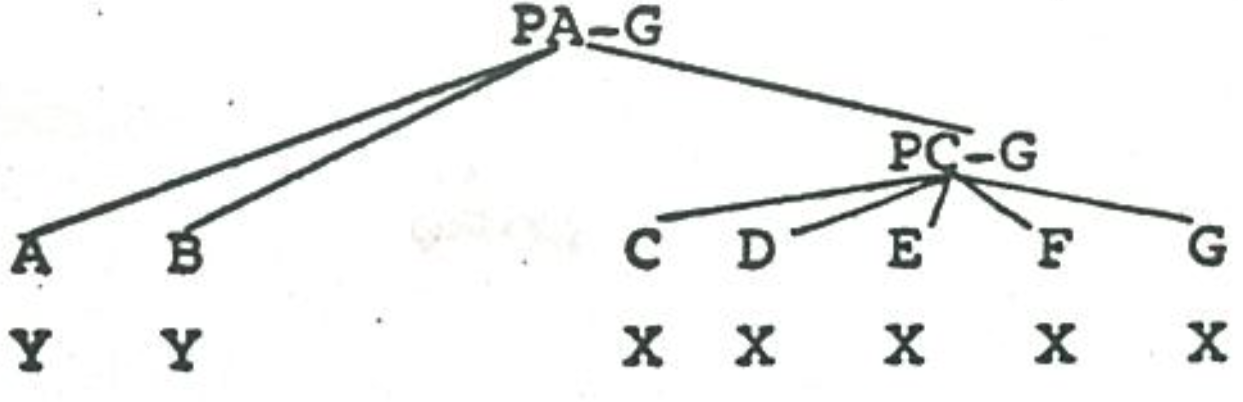
\includegraphics[width=8cm]{illustrations/Clark_1977_tree.png}
\caption{{Tree from \citet[19]{clark1976aspects} illustrating Maximum Parsimony.}}
\label{fig:clark_tree}
\end{figure}

It is important to note that Maximum Parsimony does not take into account branch lengths, only the changes between each node of the tree (regardless of how far apart they are). Furthermore, Maximum Parsimony makes the assumption that the slowest rate of change is the accurate one. %This is unlike Maximum Likelihood which does take into account branch lengths and allows rates of changes to be dynamically estimated.



%Integral to the reconstruction of forms in historical linguistics is \textbf{Maximum Parsimony}. Maximum Parsimony is a method of reconstruction ancestral states (in this case grammatical features of proto-languages) in such a way that there is as few changes as possible from the root to every tip (language). 


Reconstruction in historical linguistics also includes judgements of plausibility. This requires some assumptions about what are plausible features to co-occur in language, and which pathways of language change are more plausible than others. For example, it is rare to find a language that has a gender distinction in first person but not in third (though not impossible; c.f. \citet{wals-44}). If the most parsimonious reconstruction results in a proto-language with many rare features, it may require more investigation. Similarly, changes from certain states to others are assumed to be less plausible. For example, a language going from having no marked dual number on nouns to having trial number would be taken as unusual by most linguists (c.f. \citet[8]{kikusawa_2006_pro_number}). 

Plausibility is important in reconstruction, both in linguistics and in biology. However, this principle is sensitive to differing assumptions and theories. Besides debates over precise sub-groupings, many arguments in historical linguistics relate to this issue. For example, \citet{clark1976aspects} disagrees with \citet{hale_1968}, \citet{hohepa_1969}, and \citet{chung1978} on the state of Proto-Polynesian syntax on these grounds. Chung, Hale and Hohepa argue for a theory that is less technically parsimonious, but which they say is more plausible. They posit that Proto-Polynesian had a nominative-accusative case marking system\footnote{Hale, Hohepa and Chung actually suggest three different specific theories for this reconstruction. For a summary of the differences between the proposals, see \citet[247-249]{chung1978}.}. If this was the case, given the distribution of languages that would mean positing more changes along the tree than if we assumed, as \citet{clark1976aspects} does, that the Proto-Polynesian language was ergative-absolutive. 

Chung's plausibility critique of Clark's proposal is three-fold: 
\begin{enumerate}[label=(\alph*)]
\item the tree used is not an accurate representation of the language history (there was more interaction between S\={a}moan and Tongan)
\item it is possible that the Proto-language contained variation and was undergoing change that was only fully realised in some of the daughters\footnote{The reason that only some daughter languages exhibit the feature could be due to founder effects (my addition).} 
\item the morpho-syntactical historical process is less plausible
\end{enumerate}

In a review of \citet{clark1976aspects}, Chung writes:

\begin{quotation}
\noindent\emph{Such an approach [as Clark's] relies on the assumption that the subgroups have developed quite independently once they split off from Proto-Polynesian, so that features shared by both must be attributed to the Proto-language. But in fact, both parts of this assumption are too strong. It is well known that the two primary subgroups of Polynesian did not develop totally separately; there was long-standing contact in pre-European times between speakers of Tongic and some Samoic-Outlier languages, as Clark himself notes (p. 27). Further, and more generally, it is simply not true that every feature shared by related languages must have existed in the Proto-language uniting them. Languages are constantly undergoing change; and it is reasonable to suppose that Proto-languages were no different from real languages in this respect. But if this is so, then it is also reasonable that changes begun in a Proto-language may have continued even after its separation into daughter languages. In this way, related languages may come to share a feature which existed only in embryonic form, or not at all, in their common ancestor.}
\end{quotation}
\begin{flushright} \citet[539]{chung1977aspects}  \end{flushright}

This debate contains more twists and turns, with each side arguing for the plausibility of their accounts. In our analysis, we will be using a tree that represents the history of the languages in a similar way to Clark, which means the results are sensitive to the same critique by Chung. We are also not able to use plausibility in our computational reconstructions since we do not have access to formalised data on what plausible language profiles or changes are. This is a key difference between computational reconstruction and traditional approaches to reconstruction. Knowledge of plausibility and how to weight different kinds of evidence against each other is not formalised and cannot be taken into account.

It is possible that with the added information on rates of change and branch length that comes with the Maximum Likelihood approach we are able to approximate historical linguists' knowledge of plausibility. In that case, we would expect the Maximum Likelihood results to concur more with the predictions by expert linguists. If historical linguists mainly do operate on the same principles of Maximum Parsimony, and/or Maximum Likelihood is not able to approximate plausibility, we would expect the results of Maximum Parsimony to concur more with findings in traditional historical linguistics.

%can fall short of reconstructions carried out by classical historical linguists because they are able to take these plausibility considerations into account.

The processes of subgrouping and reconstruction are done in tandem in historical linguistics. Subgroups are proposed based on shared innovations. In order to determine what is and what is not an innovation, a certain amount of reconstruction is necessary. In order to make reconstructions, some of the tree structure needs to be approximated. 

Pawley (personal correspondence) notes that most of the subgrouping done in historical linguistics tends to be at the lower level. This can be seen later in this chapter in the difference between the Glottolog tree (Fig. \ref{tree_coverage_oceanic_glottolog}) and the Gray et al 2009-tree (Fig. \ref{tree_coverage_oceanic_gray}). Most of the splits in the Glottolog tree occur close to the tips, whereas the splits are more spread out over the distance between the root and the tips in the Gray et al 2009-tree.

Besides parsimony and plausibility, it is also important to know how to weight evidence when conducting historical linguistics research, in particular when it comes to subgrouping. This is less often discussed explicitly, but it is related to issues of plausibility and is likewise a source of disagreement. 

As was discussed in \ref{sec:dep}, not all data-points are independent of each other and this may be one reason to weight them differently. It is also possible that certain data-points are more susceptible to contact-induced change than others, and should therefore carry less weight if we are trying to infer a family tree. This is why particularly stable items are used in reconstruction and subgrouping (c.f. \citet{pawley_2009_solomons}).

For example, \citet{wilson_whence} presents a case for Eastern Polynesia (EP) being settled from the so-called ``Northern Outliers'' (i.e. Polynesian languages of Micronesia and the Solomons) by demonstrating shared innovations of lexicon and grammar to the exclusion of Samoa, Pukapuka and Tokelau (which were closer to EP in previous proposals). The paper lays out 73 innovations in support for this theory, and states that there is a lack of shared innovations supporting grouping Eastern Polynesia and the Samoic group together, as had been previously suggested by \citet{pawley1966polynesian}. \citet{wilson_whence} proposes that a more accurate reflection of this data is to group Eastern Polynesian with the Northern Outliers. On the other hand, \citet[53, 61]{pawley1966polynesian} presents two cases where Samoan and some of the Northern outliers shared features to the exclusion of Eastern Polynesia (sing/plural distinctions in indefinite articles and the form of the human number prefix). Besides the sheer number of data-points, it is clear that historical linguists also weight different pieces of information differently. Without an internalised in-depth knowledge of these matters, it is difficult to know how to evaluate the support for these conflicting theories of the origins of Eastern Polynesian communities. Is it as significant that the Northern Outliers and Eastern Polynesian languages shared a word for a certain kind of fish (\emph{*kamakama}) as the fact that they have also as a group added an \emph{o-} to the Proto-Polynesian root \emph{*fia} (want) \citep{wilson_whence}? 

In this chapter we are not proposing any new subgroupings, so the problem of weighting evidence is not present. We are, however, reconstructing grammatical features and this is another area where weighting is relevant. All languages are weighted the same for the reconstruction and the stability measurements. The tree structure and the method (Maximum Parsimony or Maximum Likelihood) determines the reconstruction. This can be compared to weighting evidence from oversampled areas/subgroups less when reconstructing. Likewise, all features contribute to the conservatism measurement per language.

% \citet[135]{marck2000} also presents the case that the Northern Outliers are most closely related to Tuvaluan.

%It is clear that considerable experience and meticulous considerations are needed in order to make these judgements and interpret the results of these papers appropriately. This entails long periods of training and familiarisation with the method in practice and the particular languages in question. \citet[721-731]{blust2013austronesian} suggests that we should bring in non-linguistic evidence to bear on these theories as well. How would a settlement from the Northern Outliers be achieved materially? By finding supporting or conflicting evidence from other disciplines, we can make more robust predictions 

%For full disclosure, both of the trees used in this study (Glottolog 4.0 and \citet{grayetal_2009}) group EP closer to the Northern Outliers than to Samoan, and it is becoming more accepted. 


%\subsubsection{Characteristics of language structure as data}
%\label{diff_lexi_str}

The Comparative Method is most often applied to vocabulary, but it can also be applied to grammatical morphemes. \citet{crowley1985common} for example traces the history of a common noun phrase marker \emph{*na/*a} in Oceanic languages using the Comparative Method. 

The data in this chapter does not track specific forms, as is common when reconstructing Proto-languages in historical linguistics (c.f \citet{pawley1973some, crowley1985common, evans2003study}). Instead we have a questionnaire that covers large parts of the grammatical domains commonly found in language descriptions in terms of structural features (see section \ref{grambank}). There are some crucial differences between structural data and the kind of data that is used in historical linguistics in relation to the present study.

The kind of data used in grammatical reconstruction in historical linguistics differs from what we find in linguistic typological questionnaires such as Grambank. \citet{crowley1985common}, \citet{clark1976aspects}, and other scholars whose work we will compare to our results in this chapter, typically apply the comparative method to specific formal expressions of structural features (the \emph{na} article, \emph{-Cia} suffix, \emph{faka-} prefix etc). They take into account fossilised forms (the common noun marker \emph{-a} fusing to roots in Paamese \citep[141]{crowley1985common}) and related meanings (the hypothesis of \emph{-Cia} changing from a transitivising suffix to a marker of passive voice (\citet{hale_1968, hohepa_1967, hohepa_1969, chung1978} and \citet{jonsson1998}). The Grambank dataset, however, (as many other typological surveys) only considers productive patterns and does not include information on specific formal expressions of grammatical phenomena.

As has been discussed earlier in this thesis (section \ref{subsection:comp_lex_str}), it is important to note that two languages can be coded identically for a structural feature in a typological questionnaire due to entirely different reasons and without being related. For example, Koasati [koas1236] of Louisiana, USA, and Mokilese [moki1238] on Mwoakilloa in the Federated States of Micronesia are both coded as having a construction for predicative possession of the type ``Topic'' by \citet{wals-2011-117}. However, they belong to entirely different language families and different parts of the world. This is unlike cognacy data, where the fact that two languages have cognates in common is direct evidence of relatedness.

An example of the differences between the structural data used in classical historical linguistics and typological questionnaires is the definite marker in Oceanic. \citet{crowley1985common} investigates common noun phrase markers\footnote{This term is more or less identical to a pre-nominal definite/specific article.} in Oceanic and finds that in many languages there is a reflex of proto-Oceanic \emph{*na/*a}, but that in some languages there is another marker with a different origin (M\={a}ori \emph{te} for example). In Crowley's study, languages where there is no common noun phrase marking whatsoever and those with a marker which is not cognate with \emph{*na/*a} are both included in type 1 (see Fig.~\ref{fig:crowley_map}). These languages are contrasted with those that have retained some kind of reflex of \emph{*na/*a} (type 2-4 in Fig.~\ref{fig:crowley_map}). This means that we can distinguish languages which have retained the proto-form from those that haven't, but not languages which have a common noun phrase marker from those that do not.

\begin{figure}
\centering
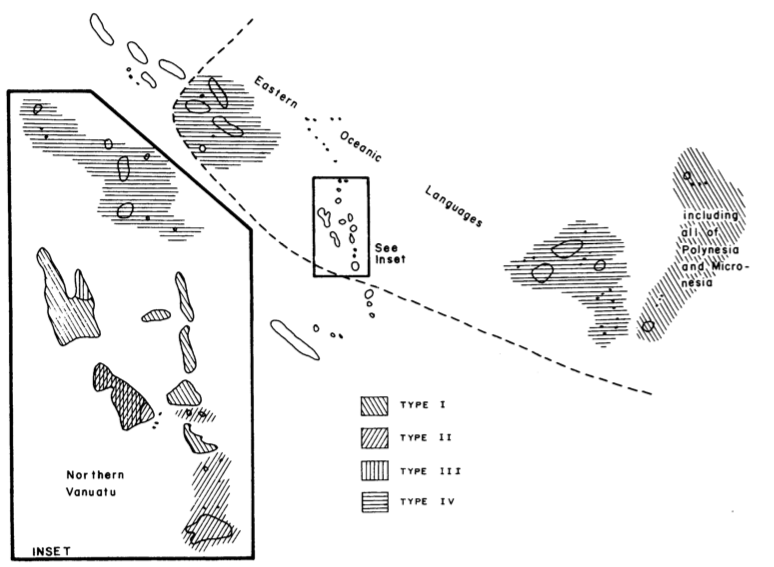
\includegraphics[width=8cm]{illustrations/crowley_1985_map.png}
\caption[Map of four different types of common noun phrase markers in Oceanic from Crowley(1985).]{\textbf{Map of four different types of common noun phrase markers in Oceanic from \citet[162]{crowley1985common}. Type 1: absence of common noun phrase marker or marker is not a reflex of \emph{*na /*a}, type 2: non-productive system involving a reflex of \emph{*na /*a}, type 3: productive marking involving \emph{*na /*a} as a prefix that is regularly separable from the noun and type 4: productive marking involving \emph{*na /*a} generally existing as a free-standing marker.}}
\label{fig:crowley_map}
\end{figure}

In contrast, the corresponding feature in Grambank is `GB022: \emph{Are there prenominal articles?'} (see Fig.~\ref{fig:gb022_map}). Languages that have \emph{te} (like M\={a}ori) or reflexes of \emph{*na/*a} as articles before the noun both count as ``yes'' (1) for GB022 and those that have no prenominal marker as a ``no'' (0). This Grambank feature splits Crowley's type 1 into two categories, and combines all the languages with reflexes of \emph{*na/*a}, \emph{te} or other markers into one category. We can now distinguish those that have a pre-nominal article from those that do not, but we cannot tell apart those which have retained the proto-form from those which have not. Since many reconstructions of grammar in historical linguistics rely on explicit formal evidence, this is an important difference.

\begin{figure}
\centering
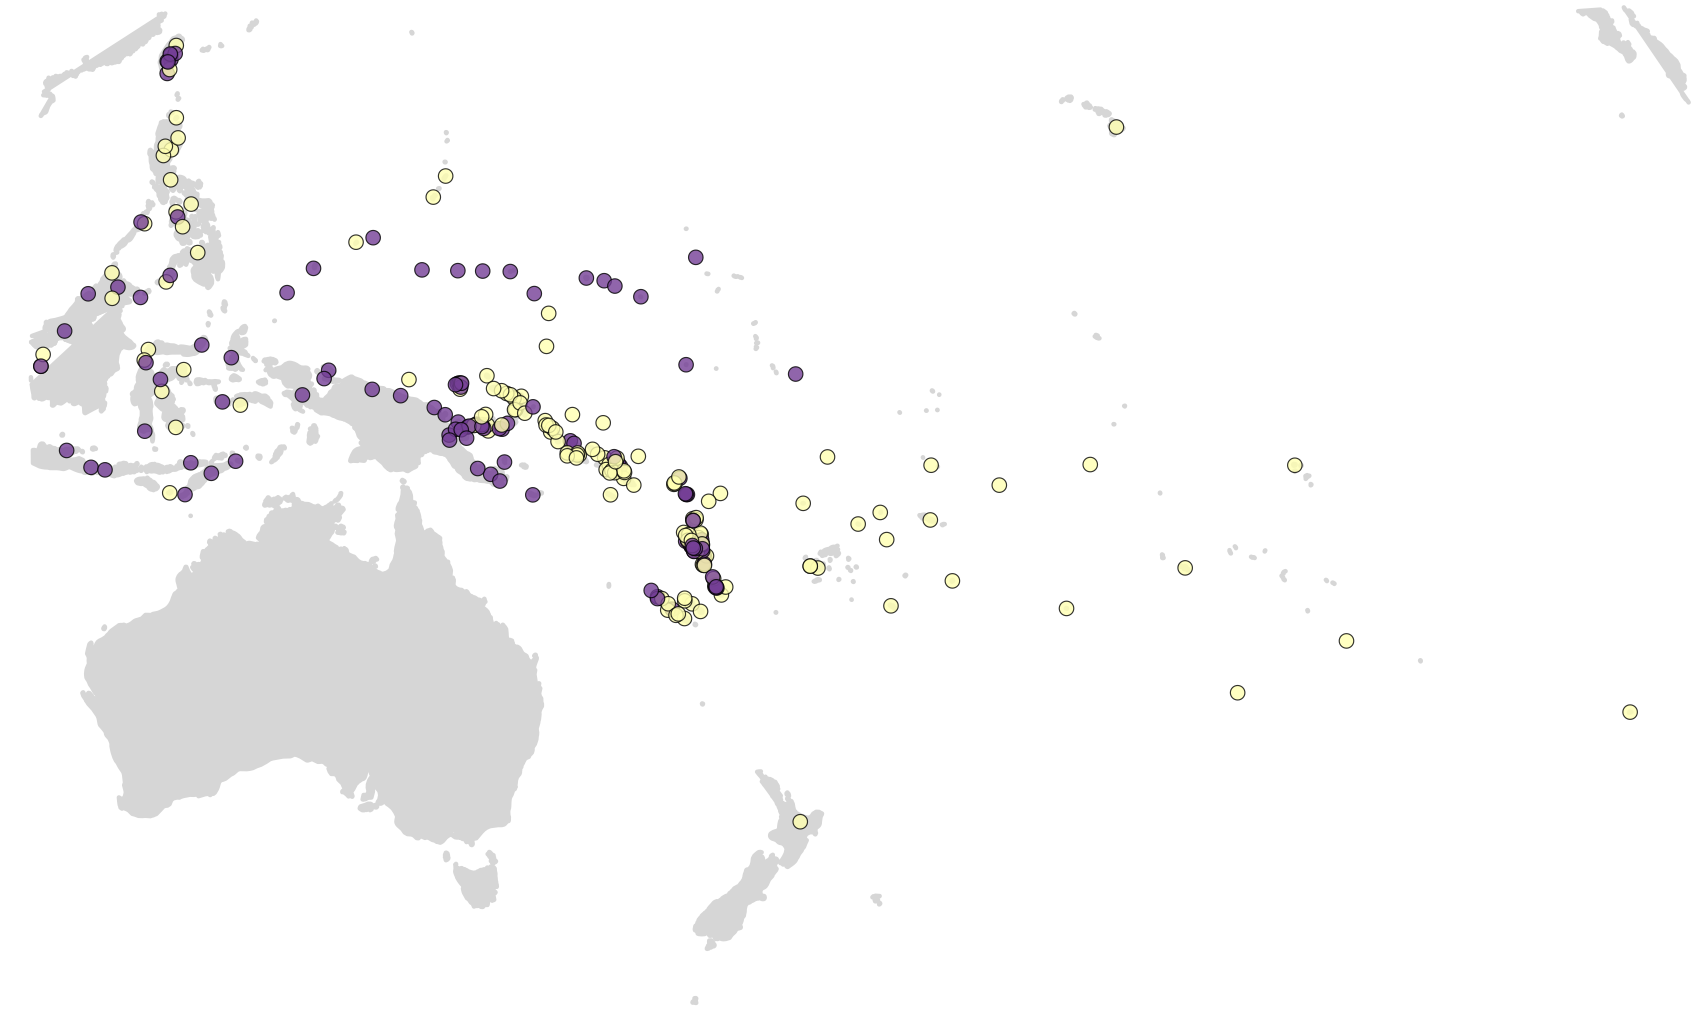
\includegraphics[width=12cm]{illustrations/plots_from_R/map_GB022.png}
\caption{{Map of Austronesian languages for GB022 \emph{Are there prenominal articles?} Yellow = "yes", purple = "no".}}
\label{fig:gb022_map}
\end{figure}

%In conclusion, the Comparative method in Historical Linguistics contains Maximum Parsimony and information on Plausibility. This study will use both Maximum Parsimony and Maximum Likelihood approaches, we expect that the findings in historical linguistics concur more with those of Maximum Parsimony than with Maximum Likelihood. The type of data used in historical linguistics is typically specific markers rather than structural features. In the case of the Oceanic subgroup, structural features will often track specific markers as well, but not necessarily.

%Furthermore, it is possible that due to the interconnectedness of structural features related languages can develop similarily without 
Related languages may also show similarity due to inheritance, even if the relevant state wasn't present in the ancestor, as the quote from \citet{chung1977aspects} earlier continues:

\begin{quotation}
\noindent\emph{[I]t is also reasonable that changes begun in a Proto-language may have continued even after its separation into daughter languages. In this way, related languages may come to share a feature which existed only in embryonic form, or not at all, in their common ancestor}\footnote{This idea is important to a particular hypothesis about Proto-Polynesian syntax, because according to \citet{chung1978} Proto-Polynesian was accusative and Tongan and S\={a}moan both developed ergativity semi-independently while the Eastern Polynesian languages (which are more closely related to S\={a}moan than to Tongan) did not develop this feature.}.
\end{quotation}
\begin{flushright} \citet[539]{chung1977aspects} \end{flushright}

This theory proposes that the conditions for developing a certain feature may have been present in the ancestral language even if the feature itself is absent. It is therefore likely that the daughter languages would develop it even if they were isolated from each other, because they have inherited the prerequisites for developing the feature. This is similar to what is known in the literature on cultural evolution as ``preadaptation'' \citep{scott2010language}. One might say that the seed is sown already in the parent language, and that as a result its daughter languages will likely turn out a certain way.

This ties in with the dependencies of features, insofar as dependencies are representations of features ``moving as a group'' through time. If some of these features are reliable ``early movers'', one could use them to predict certain developments in daughter languages. This theory aligns well with a view of language as a system where everything neatly fits (``La langue est \emph{un système où tout se tient}'' [language is systematic / a system where everything fits], Saussure \citep{koerner1997notes}). This is in contrast to the view by, among others, \citet[328]{bloomfield1933language} who stated that \emph{every word has its own history}. It is likely that systematic effects like these are more probable in structural data than in lexical data.

However, in this analysis we are investigating each feature separately so it is not possible to derive information about features co-evolving. It is also difficult for the algorithm \emph{not} to reconstruct a certain state in the parent language, if the majority of daughter languages possess it. This is one instance where knowledge of plausible paths and profiles of languages from classical linguistics may contribute information that is, so far, not possible to retrieve using computational means.

In summary, the comparative method of historical linguistics involves Maximum Parsimony coupled with information on plausibility. It is not possible in computational reconstruction to take plausibility into account since it has not been formalised. The kind of data typically used in reconstruction of grammar in historical linguistics concerns specific forms, whereas the data for this chapter is structural features.



\subsubsection{Findings from historical comparative linguistics on Proto-Oceanic grammar}
\label{sec:POC_lit_review}

The Proto-language of the Oceanic subbranch of the Austronesian language family is well researched in terms of its lexicon and phonology (see the book series on the Proto-Oceanic lexicon \citep{protooceanicvol1, protooceanicvol2, protooceanicvol3, protooceanicvol4, protooceanicvol5}, among other publications). There is also substantial work done on the grammar of Proto-Oceanic using the comparative method in historical linguistics. In this chapter I have summarised several major works in the field and distilled their research into testable hypotheses given the Grambank data and our methods. This section gives an overview of the works included and examples of how they have been incorporated into the study. Table~\ref{HL_prediction_table_summary} lists the publications used for the reconstruction of proto-Oceanic by historical linguists in this dissertation. This aggregated reconstruction is also used in chapter \ref{chapter_distances}.

\begin{longtable}{|p{3cm}|  p{5cm}| p{4cm} | p{3cm}  | p{3cm} |}
\caption{{Table of historical linguistics publications used in this dissertation for Proto-Oceanic grammar}}
\label{HL_prediction_table_summary} \\
\hline
\textbf{Citation}  & \textbf{Title} & \textbf{Proto-Languages}  & \textbf{Domains} \\ \hline
\endfirsthead

\hline
\textbf{Citation}  & \textbf{Title} & \textbf{Proto-Languages}  & \textbf{Domains} \\ \hline
\endhead


\citet{pawley1970change} & Grammatical reconstruction and change on Polynesia and Fiji & Proto-Central Pacific  &Verbal markers and aspect particles \\ \hline

\citet{pawley1973some} & Some problems in Proto-Oceanic & Proto-Oceanic and Proto-Polynesian  & Possession, noun phrase marking, negation, verbal markers, clusivity, word order  \\ \hline

\citet{clark1976aspects} & Aspects of Proto-Polynesian syntax & Proto-Oceanic and Proto-Polynesian  & Alignment, negation, word order, possession, noun phrase marking, voice \\ \hline

\citet{chung1978}  & Case marking and grammatical relations in Polynesian languages & Proto-Polynesian  & Alignment, word order, voice, noun phrase marking \\ \hline

\citet{crowley1985common}  & Common noun phrase marking in Proto-Oceanic & Proto-Oceanic &  noun phrase marking, clusivity  \\ \hline

\citet{jonsson1998} & Det polynesiska verbmorfemet \emph{-Cia}; om dess funktion i Samoanska & Proto-Polynesian & Verbal marker \\ \hline

\citet{marck2000_encyclo} & Polynesian languages (in Facts About the World's Languages: An encyclopaedia of the world's major languages, past and present)& Proto-Central Pacific and Proto-Polynesian & Word order, verbal markers, possession, clusivity \\ \hline

\citet{evans2003study} & A study of valency-changing devices in Proto Oceanic & Proto-Oceanic & Verbal markers \\ \hline

\citet{kikusawa2001rotuman} & Rotuman and Fijian case-marking strategies and their historical development  & Proto-Oceanic & Possession, pronominal number \\ \hline

\citet{kikusawa2002proto}  & Proto Central Pacific ergativity: Its reconstruction and development in the Fijian, Rotuman and Polynesian languages & Proto-Central Pacific   & Alignment, word order \\ \hline

\citet{lynchrosscrowley_proto_grammar_oceanic} & The Oceanic Languages, Chapter 4: Proto-Oceanic & Proto-Oceanic, Proto-Central Pacific and Proto-Polynesian & Negation, word order, verbal markers, clusivity, possession, pronominal number, polar interrogation, nominalisations and more \\ \hline

\citet{ross2004morphosyntactic}\footnote{This paper makes statements about ``canonical'' Oceanic languages, which is technically different from \emph{reconstruction} of Proto-Oceanic. However, the author does state that the ``canonic type is probably also a reflection of the morphosyntax of Proto Oceanic'' \citep[492]{ross2004morphosyntactic} and has given personal approval for the paper to be included in this study in this manner.}  & The morphosyntactic typology of Oceanic languages &  Proto-Oceanic and Proto-Polynesian  & alignment, word order, verbal markers, possession, noun phrase marking \\ \hline
\end{longtable}

For each of these publications, findings have been extracted that support a certain state of a Grambank feature at a certain node. For example, \citet[4]{marck2000_encyclo} writes that a causative prefix has been reconstructed for Proto-Polynesian (\emph{*faka-}). In the Grambank questionnaire we have the feature GB155 `\emph{Are causatives formed by affixes or clitics on verbs?}'. For the ancestral node that connects all the Polynesian languages, we should expect that for GB155 the state is either wholly or overwhelmingly ``yes'' (presence). For simplicity, I have only considered four ancestral languages: Proto-Oceanic, Proto-Central Pacific, Proto-Polynesian and Proto-Eastern Polynesian. The choice to focus on these four in particular was because they were the most well-researched in the literature. 

%For example,  (an ancestral language of Rotuman and Fijian separately from  Polynesian, Samoan and Northern Outliers excluding Eastern Polynesian). 

Another example of how information in the publications was turned into Grambank feature predictions relates to verbal markers encoding subjects and objects, as proposed by \citet{lynchrosscrowley_proto_grammar_oceanic} among others. In their book, there is a chapter on reconstructions of grammar for Proto-Oceanic and in the section on the basic verb phrase we find the statement below:

\begin{quotation}
\noindent\emph{Attached to the verb root were a subject proclitic and, if the verb had a non-generic object, an object enclitic.} \end{quotation} \begin{flushright} \citet[83]{lynchrosscrowley_proto_grammar_oceanic} \end{flushright}

This statement, together with a verb schema provided in the section, support the notion that Proto-Oceanic had subject proclitics and object enclitics. We can also infer from this publication as a whole that the authors believe Proto-Oceanic in fact did \emph{not} have subject \emph{en}clitics and object \emph{pro}clitics. This second prediction relies on absence of evidence and is less strong than the first, but given that the whole chapter is void of any description of object proclitics or subject enclitics being a possibility (including the verb schema) and argument structure is well-discussed, we may dare to make this leap. This information can be translated into the Grambank questionnaire by positing absence and presence for the six relevant features that concern argument marking on the verb (where S stands for subject of intransitive, A for subject of transitive and O for object; see table~\ref{example_HL_prediction_table}).

\begin{table}[H] %one of ste's favourite tables
\centering
\caption{Example of predictions from historical linguistics as rendered in Grambank features.}
\label{example_HL_prediction_table}
\begin{tabular}{|l| p{3cm}|  p{3cm}| p{3cm} | p{3cm} |}
\hline
\textbf{Grambank ID} & \textbf{Question} & \textbf{Proto-language} & \textbf{Expert prediction}& \textbf{Reference} \\ \hline
GB089  &Can the S argument be indexed by a suffix/enclitic on the verb in the simple main clause? &Proto-Oceanic &Absent & \citet[498-499]{ross2004morphosyntactic}, \citet[83]{lynchrosscrowley_proto_grammar_oceanic} \\ \hline
GB090 &Can the S argument be indexed by a prefix/proclitic on the verb in the simple main clause? &Proto-Oceanic &Present &\citet[498-499]{ross2004morphosyntactic}, \citet[83]{lynchrosscrowley_proto_grammar_oceanic}  \\ \hline
GB091 &Can the A argument be indexed by a suffix/enclitic on the verb in the simple main clause? &Proto-Oceanic &Absent &\citet[498-499]{ross2004morphosyntactic}, \citet[83]{lynchrosscrowley_proto_grammar_oceanic} \\ \hline
GB092  &Can the A argument be indexed by a prefix/proclitic on the verb in the simple main clause? &Proto-Oceanic &Present &\citet[498-499]{ross2004morphosyntactic}, \citet[83]{lynchrosscrowley_proto_grammar_oceanic}  \\ \hline
GB093  &Can the P argument be indexed by a suffix/enclitic on the verb in the simple main clause? &Proto-Oceanic &Present &\citet[498-499]{ross2004morphosyntactic}, \citet[83]{lynchrosscrowley_proto_grammar_oceanic} \\ \hline
GB094  &Can the P argument be indexed by a prefix/proclitic on the verb in the simple main clause? &Proto-Oceanic &Absent & \citet[498-499]{ross2004morphosyntactic}, \citet[83]{lynchrosscrowley_proto_grammar_oceanic} \\ \hline
\end{tabular}
\end{table}

The literature suggests that Proto-Oceanic was a language with a pre-nominal definite/specific article \citep[136]{crowley1985common}, a distinction between inclusive and exclusive first person pronouns (\citet[112]{pawley1973some}, \citet[184]{crowley1985common}, \citet[500]{ross2004morphosyntactic}, \citet[67, 75]{lynchrosscrowley_proto_grammar_oceanic}), no gender distinctions in pronouns \citep[498]{ross2004morphosyntactic}, a dual number category in pronouns (\citet[498]{ross2004morphosyntactic}, \citet[69]{lynchrosscrowley_proto_grammar_oceanic} and \citet[173]{pawley1973some}), a distinction between alienable and inalienable possession\footnote{A distinction can be made between three different kinds of possessive classification: alienable/inalienable, direct/indirect and dominant/inactive. For the purposes of Grambank and this study, these are treated as similar enough to be included into the same category.} \citep[69]{lynchrosscrowley_proto_grammar_oceanic}, prepositions (\citet[167]{pawley1973some}, \citet[498]{ross2004morphosyntactic}), subject proclitics and object enclitics on the verb (\citet[498-499]{ross2004morphosyntactic}, \citet[83]{lynchrosscrowley_proto_grammar_oceanic}), possessive suffixes on the possessed noun (\citet[495]{ross2004morphosyntactic}, \citet[155]{pawley1973some}) and a transitivising suffix on verbs (\citet[352]{pawley1970change}, \citet[171]{pawley1973some}, \citet[80, 92]{lynchrosscrowley_proto_grammar_oceanic}). More reconstructions have been made, the full table is found in the appendix \ref{asr_table_appendic}. The reconstructions regarding ergativity will be presented separately.

Most of the time, the scholars of Proto-Oceanic are in agreement in their predictions. For example, \citet[142]{pawley1973some}, \citet[292]{ross2007two}, \citet[xiii, 125]{clark1976aspects} and \citet[89]{lynchrosscrowley_proto_grammar_oceanic} all propose that the proto-language of the Polynesian subgroup had a construction marking prohibitive that was different from declarative negatives. However, in some instances there are disagreements. As discussed earlier, one such case is the alignment system of Proto-Polynesian. \citet{clark1976aspects} claims that the system was ergative while \citet{hale_1968}, \citet{hohepa_1967,hohepa_1969} and \citet{chung1978} argue that Proto-Polynesian was accusative and several of the daughter languages developed ergativity later. Crucial to this arugment is also the nature and development of passive voice in Polynesian languages. Because of this disagreement, the results for the computational ancestral reconstruction for Grambank features regarding passive voice and ergativity will be presented separately from the others. There are 109 features in the larger set of non-controversial findings, and 11 in the subset that concerns passives and ergativity\footnote{Some of these are duplicates for different proto-languages, i.e. passive voice is examined for proto-Eastern Polynesian and for proto-Polynesian.}.

In the Grambank project, research assistants read published grammatical descriptions and extract information such that it fits with the definitions of our typological questionnaire (see section \ref{grambank}). This survey of the literature on Proto-Oceanic grammar is essentially the same task. Just as with the literature on reconstructed languages, scholars sometimes disagree on the nature of contemporary languages and how they should best be analysed. It is up to the coder, in this instance me, to make calls on which analysis to employ, what can be inferred from the literature and what should be left as unknown. It is possible to squeeze even more findings out of these publications; I have tended to be conservative in my interpretations. Out of the 201 (binarised) features in our questionnaire, 31\% (63) were answerable for Proto-Oceanic given this material. The average completion per language in the whole of the dataset is 72\%. 



\subsubsection{Computational phylogenetic methods}
\label{sec:asr_methods}

In this study, we will be reconstructing the presence or absence of structural features in Proto-Oceanic using Maximum Parsimony and Maximum Likelihood. 

As discussed earlier, \textbf{Maximum Parsimony} finds the set of ancestral states that result in the fewest number of changes. Maximum Parsimony is intuitively simple. We saw in the previous section an example of how it can play out in a small tree in the work of \cite{clark1976aspects}. While Clark illustrates the principles of Maximum Parsimony well, he does not in fact use the term ``Maximum Parsimony''. %The approach is also known as ``Occam's Razor''.

Part of the critique of Maximum Parsimony is that it does not take into account branch lengths in the tree (the distance between splitting events), only the change from one node to another. Furthermore, Maximum Parsimony necessarily assumes that the solution that posits the slowest possible rate of change is the most likely one. This is not necessarily a valid assumption.

\textbf{Maximum Likelihood} posits the most likely ancestral state distributions based on the overall probabilities given all the nodes in the tree. If the distribution of values at the tips is very scattered, with sibling pairs frequently having different profiles, Maximum Likelihood will infer that the feature has a high rate of change and use that information when positing ancestral states. The Maximum Likelihood algorithm assigns probabilities of state changes and distributions differently given branch lengths. A mutation along a shorter branch is given more weight in the likelihood calculations than if it occurred in a longer branch.

In this chapter, we compare the performance of both algorithms. More technical details of Maximum Likelihood are found later in this section.

%%## begin benefits of trees
%\subsubsection{Gower-distances between languages compared to tree-modelling of rates of change}
%The \texttt{R} functions \texttt{ace()} from the package \texttt{ape} \citep{paradis2004ape} and \texttt{make.simmap()} from \texttt{phytools} \citep{revell2012phytools}

This chapter uses the same structural dataset as chapter \ref{chapter_distances} (i.e. Grambank, section \ref{grambank}), but instead of calculating distances we are applying a tree-based approach to investigate rates of change. This section outlines a few key differences between the study of this chapter and the previous.

Firstly, the aims of the studies are different. In the previous chapter we sought to explore the dissimilarity of the languages in Remote Oceania. In this study, the aim is to calculate ancestral states and the stability of features and languages. We are not generating any new distances between languages as we did in the previous chapter. The results of this study comprise ancestral states and rates of change for each variable and language, whereas the results from the study in the previous chapter concerned only structural and lexical distances between languages.

%Secondly, using a tree-based approach means that we are making use of a particular structure on our dataset, The particular trees used are of great importance as they are the basis for the calculations of rates and reconstructions. This is unlike the study in the previous chapter, where we compared languages directly one-to-one in terms of their pairwise dissimilarity.

Secondly, by using trees we are able to study the dynamics of each feature in a more realistic way. In the previous chapter the distances were calculated pairwise given all data-points (for which both had data). For each feature, a difference in value for the two languages counts as a distance of 1 and a similarity as 0. These numbers are then averaged out over the number of data-points for which the two languages were compared. A total distance of 0 between two languages mean that they are fully identical and 1 that they are entirely different. This calculation operates over all available features for two languages at a time, not taking into account any other languages nor the precise relationship between the two languages compared. 

However, the relationship between languages is interesting information. If the two languages are distantly related to each other it is possible for a feature to be absent in the shared ancestral language and still develop in both daughter languages. This could be due to chance, parallel evolution, contact or other reasons. For a particularly unstable structural feature, it is conceivable that it might flip back and forth several times from the proto-language down to each daughter language. A Gower-distance analysis of such a situation would not take this into account, since if the two languages have the same value for a given variable their distance is 0. Furthermore, it also does not consider the distribution of the feature in the rest of the sample. The distance between these two languages given this feature is the same (0) if all languages in the sample also share this feature, or if none share it. 

The analysis in the previous study was carried out over a pair of languages at a time and using all possible data. The approach in this study is instead conducted feature-wise but taking all languages into account each time (and the genealogical relationship between them). This lets us distinguish scenarios where a feature is absent in the proto-language but present in the daughter languages from those where it is present in both the ancestral proto-language and daughter languages. By positing ancestral states we can calculate a stability score per feature, and a stability score per language (the average amount of change from the root to each language over all features).

%## end benefits of trees


%\subsubsection{Method: Ancestral State Reconstruction by Maximum Parsimony and Maximum Likelihood Estimation}

We will be using two different trees of Austronesian languages, one from Glottolog \citep{glottolog40}\footnote{The tree of Glottolog 4.0 is based on work by \citet{blust_2009, blust_2014} and \citet{blust_chen_2017}.} and one from \citet{grayetal_2009}. In order for the method to function, the trees need to have branch lengths and all splits need to be binary. The tree from Glottolog does not contain information about branch lengths (all branches are the same length) and is not binary, whereas the \citet{grayetal_2009} tree has both branch length information and is binary. A part of the Glottolog tree can be seen in Fig. \ref{glottolog_example_poly}.

We can modify the Glottolog tree so that it is more appropriate for our analysis. I used the functions \texttt{multi2di} and \texttt{compute.brlen} in the R-package \texttt{ape} by \citet{paradis2004ape} to binarise and compute branch lengths respectively. Fig.~\ref{fig:branch_lengths} illustrates the process using languages of the Nuclear Polynesian subgroup in Glottolog. The tree as stored in Glottolog only contains information about subgrouping; there is no data on tree depth and therefore no branch lengths (Fig. \ref{glottolog_example_poly}.). The trees also contain non-binary splits. Fig.~\ref{fig:branch_lengths}a shows a part of this tree . The function \texttt{multi2di} randomly resolves non-binary splits until only binary ones remain, this can be seen in (b). We use Grafen's transform \citep{grafen1989phylogenetic} as implemented in \texttt{ape} to ``pull down'' all tips so that they all have the same length to the root (this is known as an `ultrametric' tree), this can be seen in (c). The final result is accomplished by first binarising the tree and then computing branch lengths (d). 

    \begin{figure}[!ht]
\centering
    \begin{subfigure}{0.45\linewidth}
      \includegraphics[width=\textwidth]{illustrations/plots_from_R/poly_tree_unscaled_multi.png}
    \caption{Non-binary splits occur, all branches have the same length.}
    \label{glottolog_example_poly}
    \end{subfigure}
\hfil
    \begin{subfigure}{0.45\linewidth}
          \includegraphics[width=\textwidth]{illustrations/plots_from_R/poly_tree_unscaled_di.png}
     \caption{Non-binary splits have been resolved to binary, all branches same length}
    \end{subfigure}

    \begin{subfigure}{0.45\linewidth}
     \includegraphics[width=\textwidth]{illustrations/plots_from_R/poly_tree_scaled_multi.png}
    \caption{Non-binary splits occur, all branches have been scaled so that the length from the tip to the root is the same}
    \end{subfigure}
\hfil
    \begin{subfigure}{0.45\linewidth}
      \includegraphics[width=\textwidth]{illustrations/plots_from_R/poly_tree_scaled_di.png}
    \caption{First, non-binary splits have been resolved to binary; second, all branches have been scaled so that the length from the tip to the root is the same.}
    \end{subfigure}

\caption[Four trees of Nuclear Polynesian demonstrating binarisation and imputing branch lengths.]{Four trees of Nuclear Polynesian languages from Glottolog, illustrating the process of binarization and imputing branch lengths.}
    \label{fig:branch_lengths}
    \end{figure}
    
Family trees in historical linguistics are often under-specified for branch lengths. For example, the publications that underlie the Glottolog tree (\citet{blust_2009, blust_2014} and \citet{blust_chen_2017}) do not contain information on the relative branch lengths, only which languages are in which subgroup. It has been said that ``linguist don't do dates'' (\citet{mcmahon2006linguists} and \citet{gray2011language}). This reflects the disappointment with early lexicostatistics which included failures at predicting language splitting events in time. However, it is possible to do relative branch lengths without dates. Given that all languages we now observe exist in the present, it seems fair to assume that an equal amount of time has passed from each of them to the proto-language. This supports the transformation as shown in Fig \ref{fig:branch_lengths} from the subgrouping-only tree in Glottolog (a) to an ultrametric tree (c and d).

The Gray et al 2009-tree incorporates information from archaeology (c.f. \citet[92]{lynchrosscrowleyinternalsubgroupingoceanic}), this is one of the reasons why it has branch lengths.
    
Ancestral State Reconstruction can be done in many different ways. Three of the more common methods are: Maximum Parsimony (Occam's Razor), Maximum Likelihood Estimation and Stochastic Character Mapping. The choice of method depends on the kind of data and assumptions involved. This study utilises Maximum Parsimony (MP) and Maximum Likelihood Estimation (ML) because they are two of the most well-known and well-understood approaches. For an extensive comparison of different methods and their advantages, see \citet{joy2016ancestral}. 

\citet{jager2018using} compared three different methods of ancestral state reconstruction for lexical data: Maximum Parsimony, Maximum Likelihood and Minimal Lateral Networks. They found that reconstructions using Maximum Likelihood performed better compared to the gold standard they applied than the other two methods. The gold standard consisted of reconstructions by historical linguists, and it should be noted that it is possible that this standard may contain errors as well.

\citet{jager2018using} describe the general performance of all the computational reconstruction methods they used as ``poor''. They evaluated the methods with F1-scores, which is a harmonic mean of the precision and recall\footnote{Precision is true positives divided by True Positives + False Positives, recall is True Positives divided by False Negatives + True Positives. F1-score = 2 * ((precision*recall) / (precision + recall)) \citep{van1979information}.} of the result of each method as compared to the gold standard \citep[133]{van1979information}. 0 is the worst possible score, and 1 the best. The highest F1-score was 0.79 (Austronesian language sample, Maximum Likelihood), and the worst was 0.44 (Indo-European, Minimal Lateral Networks). We will also assess the performance of Maximum Parsimony and Maximum Likelihood with F1-scores and compare to theirs.

For Maximum Parsimony, we are using the function \texttt{asr\_max\_parsimony()} from the R-package \texttt{castor} \citep{louca2017efficient} (which is an instantiation of the method described in \citet{sankoff1975minimal}) for calculating ancestral states and stability of features. This function produces ancestral states for all nodes and reports the number of changes that was minimally required for each feature. Languages with missing data were pruned away.

For calculating the conservatism of languages a function from a different package, \texttt{acctran()} from \texttt{Phangorn} \citep{phangorn}, was used. ACCTRAN (ACCelerated TRANsformation) is a kind of parsimony analysis where changes are assigned along branches of a phylogenetic tree as close to the root as possible. This function rescales the branches of the tree in accordance with the amount of change the Maximum Parsimony analysis dictates. In order to make the results of language conservatism comparable to the results from the Maximum Likelihood analysis, the trees were re-rooted using Nanggu [nang1262] as an outgroup. Nanggu is a language of Temotu which is genealogically far removed from almost all other languages in the sample, making it a good candidate for outgroup-rooting\footnote{Another option for outgroup rooting would have been Yapese, since it is an ``Oceanic isolate''. However, Yapese is not included in the Gray et al 2009-tree so it is not possible to use as an outgroup consistently over all the sets of results.}\textsuperscript{,}\footnote{Mid-point rooting is not appropriate here since that would make for an ultrametric tree where all tips have the same distance to the root.}. The function \texttt{distRoot} from the R-package \texttt{adephylo} \citep{jombart2017package} was used to calculate the amount of change from the root to each tip, i.e. the conservatism of languages. These distances were rescaled to between 0 and 1 to make them comparable to the results from the other set of analysis.

Ancestral state reconstruction using Maximum Likelihood Estimation involves computing each ancestral state from the tips up to the root taking into account branch lengths and the joint likelihood of states given all nodes in the tree \citep{wilks1938large, fisher1912absolute, pagel1994detecting, cunningham1998reconstructing}. The Maximum Likelihood Estimation function takes a set of observations and computes the parameter distribution that maximises the likelihood given the observed data\footnote{For a gentle introduction to the concept of Maximum Likelihood Estimation, see \citet{jonny_ML}.}. This means that for every split in the tree --- every ancestral node --- the Maximum Likelihood Estimation function computes what is the most likely distribution at that point given the nature of the entire tree. ML can be modified so that it allows for different rates of change. An Equal Rates (ER) model assumes that the chance of transition from state A to state B and from B to A are equal. However, we as linguists are aware that certain features are more likely to be lost than gained so this is not a reasonable assumption. Therefore, we allow the model to estimate different transition rates for going from A to B and from B to A given the data. This is known as ``All Rates are Different'' (ARD).

When estimating ancestral states with ML, it is possible to either a) find the state at each node that maximises the likelihood (integrating over all other states at all nodes, in proportion to their probability) at that particular node (marginal reconstruction), or b) find the set of character states at all nodes that (jointly) maximize the likelihood of the entire tree (joint reconstruction). We are using marginal reconstruction in this study since it is the recommended way to deal with uncertainty in reconstruction \citep{revell_2014}. These two methods often yield similar results, but can differ, see \citet[259-260]{felsenstein2004inferring},  \citet[121-126]{yang2006computational} and \citet[5]{joy2016ancestral} for more details. For our data, a trial run of joint reconstruction did not generate drastically different outcomes.

For this study, the function \texttt{rayDISC} from the \texttt{R}-package \texttt{corHMM} \citep{corHMM} is used for marginal reconstruction of ancestral states and rates of change per feature. Missing data in Grambank for langauges included in the analysis was converted to ambiguous, (i.e ? in Grambank $\rightarrow$ 0\&1 for rayDISC()). 

For the analysis of conservatism per language, the function \texttt{optim.pml()} from \texttt{Phangorn} \citep{phangorn} was used. This function rescales the branches in accordance with the Maximum Likelihood Estimation of change along them. The process of re-scaling the tree in this manner unroots the tree; instead of having root, branches and tips, it becomes an acyclic graph of tips connected by lines of appropriate length. Unrooted trees can be re-rooted using midpoting rooting, outgroup rooting or other methods\footnote{For a visual introduction to outgroup rooting, see \href{this blogpost}{https://phylobotanist.blogspot.com/2015/01/how-to-root-phylogenetic-tree-outgroup.html} by PhyloBotanist.}. For this study, the trees were re-rooted using Nanggu [nang1262] as an outgroup. As with the Maximum Parsimony analysis, the distance from the root to each tip was carried out with \texttt{distTip} and the distances were rescaled to between 0 and 1. 

Because Nanggu was used as an outgroup to root the trees in the conservatism analysis, features which Nanggu lacked were excluded. This left 167 Grambank features which were included in the conservatism analysis. 

Concerning missing data, for both methods the trees from Glottolog and \citet{grayetal_2009} were pruned to only tips representing Oceanic languages which are also found in Grambank. The match between Glottolog and Grambank is 226, the match between \citet{grayetal_2009} and Grambank is 112. For the parsimony analysis of each feature, languages with missing data were dropped from the trees in the analysis for that feature. For the Maximum Likelihood analysis tips with missing data were converted to ambiguous states. Features which could only be assigned values for less than half of the languages in the tree were excluded from the analysis.

For both Maximum Parsimony and Maximum Likelihood it is possible for a structural feature to appear and disappear several times along a lineage. This is different from cognate data where a cognate class cannot re-appear.

%
%For both trees and each two methods, the data is pruned so that only languages without missing data remain for each feature. Since the missing data varies of each feature, this means that some trees will have more tips than others. For our results, we will only be considering trees where at least half of the possible tips remain. The match between languages in Grambank and the Gray et al-tree is 128, meaning that trees with less than 64 tips are ignored. For Glottolog, the match was 198, so trees with less than 96 tips are discarded.
%
%%
%The ML method produces ancestral states for all nodes (see Fig.~\ref{GB409_ACR_tree}, transition rates with standard deviation errors and a Maximum Log-likelihood estimation of the entire tree per feature. In our example here, we are looking are GB409 which is concerned with the presence Ergative patterns of argument marking.The tree in Fig.~\ref{GB409_ACR_tree}, shows the estimated distributions of the two values (present or absent) in the ancestral nodes as piecharts. Most ergative ancestral states are found in a few languages of New Caledonia and also in Polynesia. The root node represents the proto-language of the entire Oceanic group and it is unlikely that it was ergative. The graph in Fig.~\ref{GB409_ACR_graph} shows us the transition rates, and we see that we are much more likely to transition from a 1 (``yes'') to a 0 (``no'') than vice versa. This means that we are more likely to lose ergativity than gain it. 



%\newpage
%\begin{figure}[H]
%\centering
%\includegraphics[width=\textwidth]{illustrations/plots_from_R/ASR/glottolog_tree_binary/ACE/tree/GB409.png}
%\caption{{Tree of Maximum Likelihood Ancestral State Reconstruction of GB409: Ergative. Yellow (light) = Yes, Purple (dark) = No}. Maximum Likelihood Estimation with Glottolog-tree}
%\label{GB409_ACR_tree}
%\end{figure}
%
%
%\begin{figure}[h]
%\centering
%\includegraphics[width=10cm]{illustrations/plots_from_R/ASR/glottolog_tree_binary/ACE/transition_plots/GB409.png}
%\caption{{Transition rates of Maximum Likelihood Ancestral State Reconstruction of GB409: Ergative using the Glottolog-tree.}}
%\label{GB409_ACR_graph}
%\end{figure}

%\newpage
%\begin{figure}[H]
%\centering
%\includegraphics[width=\textwidth]{illustrations/plots_from_R/ASR/glottolog_tree_binary/parsimony/tree/GB409.png}
%\caption{{Tree of Maximum Likelihood Ancestral State Reconstruction of GB409. Yellow (light) = Yes, Purple (dark) = No}. Parsimony with Glottolog 4.0 tree}
%\label{GB409_ACR_tree}
%\end{figure}

%Now that we have familiarised ourselves with the MP and ML methods, we should devote some space to discuss what assumptions we are making by applying this method to understanding the process of change and history. We have already seen that the ML method allows us to assume that the rates of changes are not necessarily equal, which intuitively makes sense for linguistic data. We are also using \textbf{trees} to represent language history. Linguists, biologists and others who work on understanding and reconstructing the past are aware that tree models are a representation of macro-relationships and that history also contains horizontal relationships (see \citet{ritsuko2018let} among others for discussions of trees and networks in linguistics). We are not only using trees as a model for history, we are using two specific consensus trees\footnote{As a test of the robustness of the results, the analysis was also run on a random sample of the posterior of trees from \citet{grayetal_2009} as opposed to only their summary tree. This did not yield significantly different results.}, as opposed to sampling a set of trees (c.f \citet{jager2018using}). In summary, given our methods, these are the assumptions that we are making:
%
%\begin{enumerate}
%\item The transition rate between two states are not necessarily equal (ML)
%\item The solution with the overall slowest rate of change is the best one (MP)
%\item Language history can be well represented in trees (MP, ML)
%\item Language history can be well enough represented in \emph{one} tree (MP, ML)
%\item Marginal reconstruction is more suitable in this instance than joint reconstruction  (ML)
%%\item We are not loosing valuable information by binarising the tree
%\end{enumerate}



%There are other methods of ancestral state reconstruction which make use of a set of trees and incorporates uncertainty  --- Bayesian Inferential Phylogenetics (for more details on how non-Bayesian ML compares to different Bayesian approaches, see \citet{joy2016ancestral}). 


%We will also be investigating our data using a Bayesian approach --- Stochastic Character Mapping (SCM). This method was developed by \citet{hulsenbeck_2003} and operationalised and popularised through the software application SIMMAP by \citet{bollback2006simmap}. We will be using the implementation of this method in the \texttt{R}-package \texttt{phytools} \citep{revell2012phytools} in the form of the function \texttt{make.simmap()}. 

%SCM is more computationally sophisticated compared to ML, instead of reconstructing one history of the tree it reconstructs multiple (as defined by the user, in our case 1,000) and samples the most likely ancestral distributions from these. SCM does not only posit ancestral states are nodes, but also simulates changes along the branches of the tree. Fig.~\ref{hulsenbeck_fig} shows an example from \citet{hulsenbeck_2003} of 25 simulations of character changes along the same tree with the same tip values. 

%\newpage
%\begin{figure}[H]
%\centering
%\includegraphics[width=\textwidth]{illustrations/hulsenbeck_SCM.png}
%\caption{{Illustration from \citet{hulsenbeck_2003} showing 25 simulated character histories with the same observed states at the tips, equal rates of change and one substitution.}}
%\label{hulsenbeck_fig}
%\end{figure}

%As with ML, we can let the function find the transition rates instead of assuming that they are equal (ARD as opposed to ER). We are setting the number of simulations to 1,000, this allows us to explore a great possibility space. We are also asking the model to find the probability of the root note (pi = "estimated" rather than "equal"). For more details of the inner workings of SCM, see \citet{hulsenbeck_2003} and \citet{bollback2006simmap}

%The call of our function is: \citettt{phytools::make.simmap(data, tree model="ARD", nsim = 1000, pi = "estimated")}.

%\textcolor{red}{I'm considering dropping out the SCM analysis for this chapter. I've had some trouble applying it, and it's not entirely clear that it is adding something beyond what the ML results are telling is.}
%



%
%
%
%
%\subsubsection{Methodology of linguistic typology compared to phylogenetic linguistics}
%\label{sec:asr:typmetod}
%In this study, we are using data from a typological questionnaire with methodological approaches that are not commonly used in linguistic typology. This section discusses how the approach in this study differs from classical typology.
%
%Linguistic typology is a sub-discipline of linguistics which systematically compares languages, finds patterns and seeks explanations for those patterns. Typology is typically more focussed on structure than lexicon or phonology, and the data is often derived from published grammars of languages by the use of questionnaires. Based on distributions of (mainly structural) features in the world's languages, typologists draw on both language-internal and language-external factors (psychology, environmental etc) to explain the patterns observed. For example, it has been found in many typological surveys that ergative case marking pattern\footnote{Ergative case marking is a term that refers to languages where the subject of an intransitive clause is marked the same way as the object/patient of a transitive clause, and differently from the subject of a transitive clause.} are uncommon in the world's languages, \citet{Bickel_et_al_2015} suggest that this is related to the neurophysiology of the brain, that ergative case marking patterns are less intuitive and more surprising.
%
%As was discussed in section \ref{dist_chapter_str_disparity_intro}, the methodology of linguistic typology are based on \textbf{a) well-defined and meaningful cross-linguistic categories}, \textbf{b) the systematic application of those categories on the languages} and \textbf{c) sampling}. We discussed (a), (b) and (c) in section \ref{dist_chapter_str_disparity_intro}, as well as introduced the Grambank project. We will discuss (c) sampling again in this chapter as it relates to the particular methods of this study.
%
%There are many different approaches to sampling (see for example \citet{dryer1989large, croft1990, rijkhoff1993method, miestamo2016sampling}, one of them is \textbf{probability sampling}. The problems that typological probability sampling seeks to solve are that of phylogenetic non-independence (Galton's problem) and spatial auto-correlation (communities that are close to each other being similar, regardless of genealogy). Languages are grouped into genealogical units (families or genera) and geographical units (for example AUTOTYP-areas \citet{autotyp_1}), and are then selected such that no genealogical unit or area is overrepresented. A version of this method has been the dominant methodology in the field since the 1980's, with different proposals on what the exact constitution of the sample should be.
%
%%Based on the distributions and explanations, they are then able to predict what the probable distributions might be in all languages. These predictions often take the form of universals; either absolute (\emph{every language has x}) or implicational (\emph{languages that have z also have y}). Most absolute language universals have been disproven \citep{universalsarchive} and it has also been shown that some implicational word-order universals differ in strength depending on which family you are studdying \citep{dunn2011evolved, levinsonetal2011}. There has also been a movement in the field from exception-less universals to probabilistic ones (c.f. \citet{bickel_2014_universals}), which makes the counter-examples less of a problem (and perhaps even more interesting). By viewing universals as probabilistic, it is easier to integrate the predictions with other disciplines. Linguistic typology as a field is becoming more and more cross-disciplinary (almost to the point that perhaps it has ceased to exist as its own discrete ontological entity).
%
%%One way in which this trends expresses itself is in the topics of plenaries and talks of the biannual meeting of the Association for Linguistic Typology. In recent years there have been topics such as pre-historic phonology \citep{Moran_2017} and the influence of demographic pressures on language \citep{dediu_2017}.
%
%%If the questions and explanations of linguistic typology are not what defines the field, it may be that the methodology is\footnote{Some scholars have indeed noted that linguistic typology is more of a method than a field of study \citep{Dahl-1990}.}. The fundamental tools of typology is \textbf{a) sampling} and \textbf{b) good cross-linguistic categories} (given what you want to investigate), and \textbf{c) the systematic application of those categories on the sample.} We will discuss each of these in turn as it relates to Grambank and the development of the discipline at large. 
%
%%There are two kinds of typological \textbf{samples}: \textbf{probability} and \textbf{variety} samples\footnote{For novel approaches to variety sampling, see \citet{dahl_poster} and \citet{miestamo2016sampling}.} \citet{rijkhoff1993method}. Probability samples aim to represent the world's languages well statistically and for each member of the sample to be independent. Variety samples on the other hand aim to maximise the linguistic disparity, revealing even the rarest language features.
%
%%In this study, we want to have an unbiased approach to Oceanic language structure, hence ignoring variety sampling. In fact, we are not using typological sampling at all. Instead, we are using all languages that we have in our dataset and controlling for relatedness via trees. This has certain advantages, and is entirely necessary for  reconstructing the state of proto-languages . However, this approach can also be useful when conducting research on a global scale.
%
%Another approach, which is quite drastically different, to solve this problem is to include as many languages as possible and control for relatedness and areality directly by using continuous measurements of relatedness and geographic proximity as a control in the analysis. By taking pairwise distances in language family trees or geographical distance between languages directly into account, we can account for phylogenetic non-independence and spatial auto-correlation in a more fine grained way . I will be referring to this approach as distance controlled analysis\footnote{Note that this needn't be only genealogical or geographic distances, any continuous measure of relationships can be incorporated.}. This idea is borrowed from biology (which borrowed the idea of trees from linguists in the first place \citep{greenhill2015evolution}), and has had much success there. By controlling for relatedness and proximity with continuous measurements instead of discrete group membership (classical typological probability sampling), we gain two advantages: a) we needn't assume that all members of our sample are equally independent from each other and b) we are not throwing away information --- or languages for that matter. It is also possible to apply this technique to samples created by classical probability sampling, since it is unlikely that all languages in those samples are indeed equally distant from each other genealogically and/or areally. 
%
%Distance controlled analysis makes use of language family trees and geographical information. However, what to do when the tree structure is not certain or when we want to compare across families? The classical comparative method has not arrived at (and perhaps never will arrive at) a theory of the relationships between exactly all languages in the world (a ``world tree''). Historical linguists have found between 141 (Ethnologue) and 239 (Glottolog 4.0) language families in the world which are considered to be not demonstrably related to each other. If we want to compare languages globally using the distance control approach, it is necessary to have distances between all languages including those that belong to different families. This would require somehow joining these families up so that we can measure the distances between all the languages of the world. Such a phylogeny would be controversial and not justified in the same way as the structures established by classical historical linguistics. \citet[121]{grafen1989phylogenetic} suggests that in biology one should use the term ``working phylogeny'' in contrast to the (unknown) true tree structure when conducting analysis of a similar kind. This terminology may be useful for linguistics as well. The phylogenies in analyses of this kind are not necessarily proposed as a precise representation of history, but rather as a tool for investigating other research question which require the distance control approach. As such, they needn't be subjected to the same rigours standards as trees arrived at by the comparative method.
%
%There are different approaches to achieving this `working tree' of the world's languages necessary for the analysis. One approach is to take known topologies of families from established resources like Ethnologue or Glottolog and tie them together, scaling branches appropriately \citep[9]{bromham2018parasites}, \citep[9]{hua2019ecological} and \citet{verkerk2019}. The scaling of branches can be done with Grafen's transform \citep{grafen1989phylogenetic} or by using known dates as in \citep[9]{bromham2018parasites}. Another way is to use data to infer a single tree \citep{jager2016inferring}. The deeper nodes of these `working world trees' will be more uncertain than the shallower sub-groupings, but it has been argued that it is still a preferable method to using only the discrete genealogical categories otherwise popular in typology \citep{lindell_simon_course_2018} (c.f. \citet{felsenstein1985phylogenies, purvis1994truth}.). The argument is that the problem of assuming that the languages of a classical typological probability sample are independent is greater than the problem of the uncertainty of the deeper nodes of these world trees . With modern techniques, we can also sample many trees from a posterior rather than rely on only one tree \citep[31]{jager2018using}.
%
%Using distance controlled analysis instead of classical probability sampling is still new in linguistics and not widely spread. In this case, we are only considering languages of the same family --- Austronesian. This means we need not concern ourselves with world trees, but uncertainty may still impact deeper nodes in our phylogeny.
%
%%Controlling for phylogenetic non-independence is already something historical linguists practice, it is integrated into the basics of the comparative method. It is for example evident in \citet{ross2004morphosyntactic}, \citet{pawley1973some} and \citet{clark1976aspects} where the authors describe how they sample the Oceanic language tree evenly and take into account sub-groupings in their analysis. 
% 
%%It is possible to use discrete subgroup sampling (probability sampling) from typology to accomplish this as well; grouping languages into appropriate groups based on genealogy and searching for the most parsimonious solution given the distribution over these groups. However, we have more information about the relationship between languages than can be represented by allowing for only one level (or even two) of these groups. By borrowing methods from biology and controlling for the tree itself in our analysis, we need not throw away information (or languages). Historical linguists already do this in their methodology, perhaps this is why collaborations between evolutionary biology and historical linguistics has been so fruitful in the last decade (c.f. \citet{greenhill2011pollex}).
%
%%In this study we are considering data that is more coarse-grained compared to what historical linguists typically use, and instead more similar to classical structural typology. We will be using methods that will be ruthlessly uniformly applied to all data-points with no human input or editing of particulars. The data itself is the product of fieldwork, grammar writing and coding of typological questionnaires which naturally involves human judgement and editing (c.f. computational methods applied to expert coded cognacy data), but the modelling of the prior states and stability will be automatic and computational. One of the advantages of this approach is that it may be more transparent and replicable, if less nuanced and detailed compared to what a traditional historical linguist might produce. 
%%In this instance, Oceanic linguists make more distinctions that our typological questionnaire makes. 
%
%%Similarly, the notion of ``subject'' in Oceanic languages is not  (cf \citet{ross2004morphosyntactic})
%
%%Unlike traditional linguistic typology we will be controlling for genealogical non-independence with explicit trees. There is currently a debate in linguistics about the nature of cross-linguistic comparative concepts (see section \ref{intro:chapter_distances}). In our study, we use cross-linguistic categories which are defined separately from particular languages and grammar authors, but we are agnostic as to whether these should be described as ``natural kinds'' or not.
%
%%The third item in the typological toolbox is the \textbf{systematic application} of the questionnaire on the sample, which is further elaborated on in section \ref{measuring:sec:grambank} which introduces the Grambank project.
%
%%Typologists who use existing grammatical descriptions as their main source of information\footnote{As opposed to using parallel corpora, speaker surveys etc.} are at the mercy of decisions and analysis made by the particular authors. More on how we tackle this within the Grambank project in the next section.
%
%%There is the possibility that descriptive linguists working in a certain area or family have developed conventions that may cause them to exaggerate differences between languages within their group of study and those outside, and to exaggerate similarity within. 


\subsubsection{Data coverage}
\label{asr:sec:GBcoverage}
For this study, we are using binarised data from the Grambank project (section \ref{grambank}). We are focussing on Austronesian languages and the Oceanic sub-group in particular. 

The Oceanic subgroup covers almost all languages in Remote Oceania, with the exceptions of Chamorro and Palauan. As was discussed in section \ref{sec:hist}, Yapese is sometimes not included in the Oceanic subgroup and Nguluwan contains material from Ulithian and Yapese. For the purposes of this study, we have used the definition of Oceanic from Glottolog 4.0 \citep{glottolog40} and \citet[2]{protooceanicvol5} (see Fig.~\ref{Oceanic_map}). This results in Yapese and Nguluwan being included, and Chamorro and Palauan being excluded.

\begin{figure}[h]
\centering
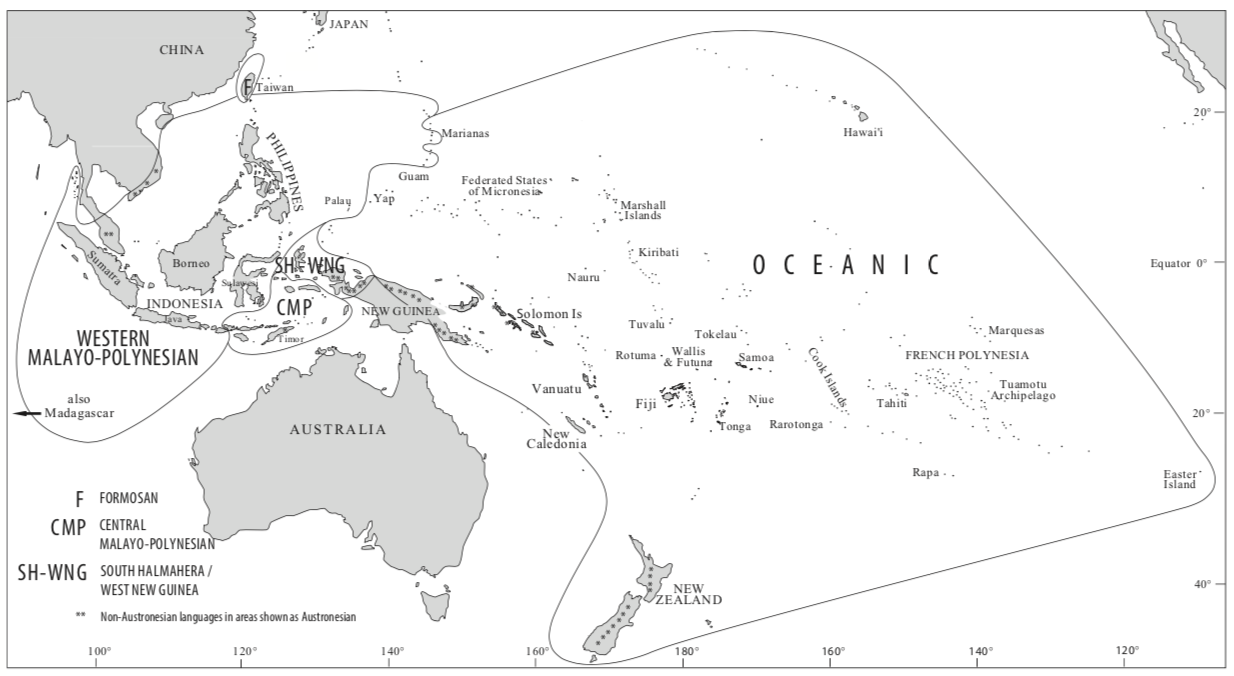
\includegraphics[width=\textwidth]{illustrations/ross_pawley_osmond_protooceanic_vol5.png}
\caption{{Map of the Austronesian language family and major subgroups, from \citet[2]{protooceanicvol5}.}}
\label{Oceanic_map}
\end{figure}



%As has been noted by \citet{crowley1985common} and others, our understanding of the Oceanic sub-group and region has in the past been biased because of oversampling of the Central Pacific Linkage (Fijian, Rotuman and Polynesian languages). This is more true of older work on the subgroup than contemporary.

The Oceanic subgroup also contains languages from Near Oceania (see section \ref{geo_intro_section:remote}) and these are included in the analysis of this chapter. These languages were grouped into three geographical groups for the conservatism analysis (section \ref{sec:conservatism}): 1) Bismarck (including Manus), 2) Solomons and Bougainville; and 3) New Guinea Mainland/Louisiade Archipelago. See Fig. \ref{Marck_map_with_language_names} in section \ref{subregion:sailing} for locations of these regions.

Table~\ref{GB_coverage_table} shows the number of languages in the Oceanic subgroup that are covered in the Grambank dataset, and which ones are possible to cover in future. Of all the languages in the subgroup, there are 261 languages that have been documented in descriptive works such that we are able to answer our questionnaire. 241 languages are currently too poorly described for us to include them in the database. As has been discussed before, it is not always possible to fill in all the features for every language. Nineteen of the Oceanic languages that are included to date are less than 50\% completed. This can be due to lack of access to descriptive work, or that the content of the descriptive work doesn't cover the necessary domains in enough detail for our coders to answer enough questions. The map in Fig.~\ref{GB_austro_coverage} shows the same coverage information for the languages of the region (including a few non-Oceanic Austronesian languages as well). 

\begin{centering}
\begin{table}[h]
\caption{{Coverage of Oceanic languages in Grambank (based on Glottolog 4.0 definition of ``Oceanic''.)}}
\label{GB_coverage_table}
\centering
\begin{tabular}{|l|l|}
\hline
\textbf{Coverage} & \textbf{Languages} \\
\hline
\textbf{\cellcolor{hedvig_orange!50}{No grammar}} &  247  \\
\hline
\textbf{\cellcolor{hedvig_blue!50}{Grammar exists, but language not in Grambank (yet)}} & 48 \\
\hline
\textbf{\cellcolor{hedvig_lightgreen!50}{Less than half of the features covered in Grambank}} &  20  \\
\hline
\textbf{\cellcolor{hedvig_darkgreen!50}{More than half of the features covered in Grambank}} &  205  \\
\hline
\end{tabular}
\end{table}
\end{centering}

\begin{sidewaysfigure}
\centering
\includegraphics[width=\textwidth]{illustrations/plots_from_R/Austro_map_desc_status.png}
\caption{{Map of Oceania, with Austronesian languages coloured for coverage in Grambank.}}
\label{GB_austro_coverage}
\end{sidewaysfigure}


In this study, we will be using two different trees to reconstruct ancestral states: one from \citet{grayetal_2009} and one from Glottolog 4.0. Figures \ref{tree_coverage_oceanic_gray} and \ref{tree_coverage_oceanic_glottolog} show the Grambank coverage of languages along these two trees. Grambank does cover a significant amount of languages east of the Solomons, but the coverage around the coast of New Guinea is still to be completed. Grambank is a work in progress, and these languages are within our target group for coverage in the near future. At this time, the coverage is less complete in the western languages compared to the eastern. However, since we control for genealogical relatedness through the distance control approach, this is less of a problem for our methodology than if we were using traditional probability sampling.

For both Maximum Parsimony and Maximum Likelihood the two trees were first pruned down to only languages where there is data in Grambank. For the further Maximum Parsimony analysis, tips representing languages where the data for a particular feature was missing were dropped for the analysis of that feature. For the Maximum Likelihood analysis, the value at such tips was converted to ambiguous. This is necessary because otherwise the rate of change across the different features would not be comparable in the Maximum Likelihood analysis.

The tree from \citet{grayetal_2009} contains duplicates (see for example Nakanai). This is because it is a tree of word-lists for languages rather than languages themselves. For the analysis, only one tip per language was retained, at random.

\begin{figure}[H]
\centering
\includegraphics[width=\textwidth]{illustrations/plots_from_R/Oceanic_tree_desc_status_gray_et_al_tree.png}
\caption{{Tree of Oceanic from \citet{grayetal_2009}, with languages coloured for coverage in Grambank.}}
\label{tree_coverage_oceanic_gray}
\end{figure}


\begin{figure}[H]
\centering
\includegraphics[width=\textwidth]{illustrations/plots_from_R/Oceanic_tree_desc_status_glottolog.png}
\caption[\textbf{Tree of Oceanic from Glottolog, with languages coloured for coverage in Grambank.}]{\textbf{Tree of Oceanic from Glottolog, with languages coloured for coverage in Grambank.}}
\label{tree_coverage_oceanic_glottolog}
\end{figure}


%The language labels are very small, this is because there are a great number of them and they cannot be larger lest they overlap. Readers who view this as a digital copy can zoom in. Readers viewing it on paper should focus on the colour rather than the letters.}

%The language labels are very small, this is because there are a great number of them and they cannot be larger lest they overlap. Readers who view this as a digital copy can zoom in. Readers viewing it on paper should focus on the colour rather than the letters.)


\newpage
\section{Results}
The results of this study are divided into three parts:

\begin{itemize}
\item Concordance between computational reconstructions and findings in traditional historical linguists
\begin{itemize}
\item the ergativity in proto-Polynesian-issue
\end{itemize}
\item Stability of features
\item Conservatism of languages
\end{itemize}

In this study we are using two trees (Glottolog 4.0 and \citet{grayetal_2009}) and two models (Parsimony and Maximum Likelihood Estimation), making for a total of four sets of results. Trees with more than half of the possible tips missing are discarded. The match between languages in Grambank and the Gray et al-tree is 112, meaning that results with less than 56 tips are ignored. For Glottolog, the match was 226, so results with less than 113 tips are discarded.

%As was discussed earlier, there were 9 features that were not possible to include in the ML results because the model requires a minimal level of change. These are all found in table~\ref{GB_all_or_nothing} and for all of them the Parsimony results predict absence at the root


%We will return to these in section \ref{sec:most_like_austro}.

%For our set of predictions from historical linguistics, there is only one feature on one tree where we were unable to calculate the ML ancestral states: GB260 combined with the Gray et al 2009-tree. Over our 109 (non-ergativity) predictions this means that we have 435 results to evaluate for the comparison with traditional historical linguistics.

All results have been calculated in \texttt{R} \citep{R} using the packages \texttt{castor} (Parsimony) \citep{louca2017efficient}, \texttt{phangorn} \citet{phangorn}, \texttt{adephylo} \citep{jombart2017package}, \texttt{corHMM} \citep{corHMM}, \texttt{ape} \cite{paradis2004ape} and phytools \citep{revell2012phytools} and tidyverse \citep{tidyverse13}.

\subsubsection{Concordance with traditional historical linguistics}
In this section we compare how often the computational reconstructions are in concordance with those made by historical linguists. For each feature, the algorithm predicts a distribution of the two states (presence and absence) for every ancestral node. If the distribution is majority presence (more than 60\% of the ancestral state is ``1'') it is registered as ``Presence''; if less than 40\% presence it is registered as ``Absence''. If the ancestral state is between 40-60\% of either state, the prediction is registered as ``Half/Half''. If the reconstruction of a feature by experts for that ancestral node was ``Presence'' and the algorithm did predict presence with over 60\%, it is a ``True positive'', and so on. Table~\ref{example_HL_prediction_table_true_positives} illustrates how the results are calculated.

\begin{table}[H]
\centering
\caption{Table illustrating how the results of ancestral node predictions are calculated.}
\label{example_HL_prediction_table_true_positives}
\begin{tabular}{|l|l|l|l|l|l|l|l|}
\hline
\textbf{Finding in historical linguistics} & \textbf{Prediction by MP or ML} & \textbf{Result} \\ \hline
Presence & >60\% Presence & True Positive \\ \hline
Presence & >60\% Absence & False Negative (type 2-error) \\ \hline
Absence & >60\% Absence & True Negative \\ \hline
Absence & >60\% Presence & False Positive (type 1-error) \\ \hline
Presence & 40-60\% Presence/Absence & Half/Half\\ \hline
Absence & 40-60\% Presence/Absence & Half/Half \\ \hline
\end{tabular}
\end{table}

In order to evaluate the results, we need to calculate a concordance score per method and tree. \citet{jager2018using} use the F1-score (harmonic mean between precision and recall) in their study of how computationally reconstructed lexical proto-forms compare to those reconstructed by historical linguists.  For example, if for a given proto-language there are 60 features reconstructed by experts and the algorithm result is 10 True Positives, 10 False Positives, 10 True Negatives, 10 False Negatives and 20 ``Half/Half'' then the F1-score is 0.5 (recall = 10 / (10+10) = 0.5, precision = 10 / (10+10) = 0.5 and F1-score = 2 *((0.5*0.5) / (0.5 + 0.5) = 0.5)). %Note that the F1-score disregards True Negatives and Half /Half-results.

F1-scores will be reported because they are insightful and have been used in similar studies. However, the F1-formula ignores the amount of True Negatives and Half/Half results. Therefore, in addition we will also calculate a simpler concordance score; how many concordant predictions did the algorithm make given all the predictions it made (aka ``accuracy'')? For example, if for a given proto-language there are 60 features predicted by experts with the same distribution of results as in the example above, then the concordance score would be (10 + 10)/40 = 0.5. We can also include the Half/Half-predictions, awarding 0.5 points for at least not strongly predicting a false value. In that case, this example has a concordance score of 0.5 ((10 + 10 + (20/2)) / 60). These scores all reflect different ways of assessing concordance and will give different perspectives on our results and how our algorithms are performing. %Features where there were more than half of the data-points missing in the tree were not to be included. hankfully there were no occurrences of this.

The full table of all predictions (excluding those relating to ergativity) and all results per feature, tree and method can be found in table~\ref{asr_table_appendic} in appendix \ref{ASR_comparison_table}. The summary results for the concordance with reconstructions by experts from historical linguistics are presented in table \ref{reconstruction_summary_table}. 
 
\begin{table}[H]
\centering
\caption{Comparison of how often the computational ancestral state reconstruction agrees with reconstruction from historical linguistics literature.}
\label{reconstruction_summary_table}
\begin{tabular}{|p{5cm}| p{2cm}|  p{2cm}| p{2cm} | p{2cm} |}
\hline
& \multicolumn{2}{c|}{Glottolog 4.0-tree}& \multicolumn{2}{c|}{Gray et al (2009)-tree}\\ \cline{2-5}
& \textbf{Parsimony} & \textbf{Maximum Likelihood} & \textbf{Parsimony} & \textbf{Maximum Likelihood} \\ \hline

 \cellcolor{hedvig_lightgreen!50}{Agree} &92&29&92&56\\ \hline
\cellcolor{hedvig_red!50}{Disagree} &9&2&11&7\\ \hline
 \cellcolor{hedvig_yellow!50}{Half / Half} &8&78&6&46\\ \hline

 \textbf{Accuracy score (incl Half/Half)} &0.88&0.62&0.87&0.72\\ \hline
 \textbf{Accuracy score (excl Half/Half)} &0.91&0.94&0.89&0.89\\ \hline
\cellcolor{hedvig_red!50}{False Negatives} &5&1&5&4\\ \hline
 \cellcolor{hedvig_lightgreen!50}{True Negatives} &42&8&41&17\\ \hline
\cellcolor{hedvig_red!50}{False Positives} &4&1&6&3\\ \hline
 \cellcolor{hedvig_lightgreen!50}{True Positives} &50&21&51&39\\ \hline
\textbf{Precision}&0.93&0.95&0.89&0.93\\ \hline
\textbf{Recall}&0.91&0.95&0.91&0.91\\ \hline
\textbf{F1-score} & \textbf{0.92} & \textbf{0.95} & \textbf{0.9} & \textbf{0.92} \\ \hline

\end{tabular}
\end{table}

One of the most striking features of these results is the number of Half/Half predictions in the ML results. The ML approach takes into account the overall likelihood of the entire data, and for our dataset and trees this leads to more Half/Half results compared to the parsimony approach. One way of interpreting this is that the ML is more careful, it makes fewer confident predictions (more than 60\% either way), but it also disagrees less often with the findings from historical linguistics.

As was discussed earlier, there are several different ways of evaluating the performance of these approaches. If we consider how often they made a prediction that agreed with historical linguistics out of all the times they made a confident prediction (Accuracy score excl Half/Half), then ML paired with the Glottolog tree does best. If we award half a point for Half/Half predictions, Parsimony paired with the Glottolog tree does best. Overall, the results using the Glottolog-tree agreed more often with historical linguistics than did the analysis with the Gray et al 2009-tree.

We are comparing our computational reconstruction results to those predicted by expert linguists. The reason that the Glottolog tree is more in line with the predictions from historical linguistics is probably because it resembles the tree most historical linguists are used to more than the Gray et al-2009 tree does (the Glottolog tree is based on \citet{blust_2009,blust_2014} and \citet{blust_chen_2017}). That is not to say it is necessarily a better reflection of the true history of these languages, but rather that it may fit better with the underlying model that the field of historical linguistics has been working with in recent decades. Most of the literature on reconstructions of Proto-Oceanic does not include detailed accounts of the exact tree topologies and branch lengths used to reconstruct the ancestral languages. As was shown in section \ref{sec:asr_methods}, we had to impute branch lengths for the Glottolog-tree. The manner by which reconstructions are postulated in historical linguistics is typically by considering how well distributed the phenomena are over certain genealogical and areal subgroups. If the distribution is convincingly non-random and the comparative method can be used to reconstruct forms, predictions about the proto-language are made (c.f. \citet[109-110]{pawley1973some}).

Furthermore, there were fewer matches between languages for which there is Grambank data and the Gray et al Tree, making for more uncertainty in predicting ancestral states.

In a similar study, \citet{jager2018using} attempt to reconstruct cognate classes for the proto-languages of three different language families. They used various approaches: binarising versus not binarising data; Maximum Parsimony versus Maximum Likelihood Estimation versus Minimal Lateral Networks; and using a single consensus tree versus sampling several from the tree posterior. The highest F1-score they achieved in this paper was 0.79 for the Maxmimum Likelihood Estimation reconstruction of Austronesian (using either a single tree or a sample of trees). This means that all of our results above perform ``better''. While this may be pleasing, it is not yet entirely clear why this is. 

In this study, only statements about ancestral languages that could be mapped to Grambank-features were included. It is  possible that the \citet{jager2018using} study had a greater overlap between all the reconstructions made by historical linguists and the meanings that they had data for. It is also possible that the set of features that were possible to include were also somehow easier to reconstruct, and if so that would explain the higher F1-scores.
%\label{sec:ars:metod:hist}

Many of the features that have been reconstructed for proto-languages of the Oceanic subgroup are also very common among Oceanic languages. For example, in our dataset 223 languages have a distinction between alienable and inalienable possession, and three do not have this feature . It is perhaps no surprise that historical linguists, Maximum Parsimony and Maximum Likelihood  agree that it is likely that the proto-languages have this feature as well\footnote{There was one exception. Maximum Likelihood on the Glottolog tree did not confidently predict presence of alienablity possession for Proto-Oceanic, the result was classified as ``half''. It did however predict alienablity for Proto-Polynesian.}. However, it is not always so simple. If this was all there was to it, we could just use raw distributions to reconstruct features of proto-languages. Historical linguists stress the importance of Maximum Parsimony and plausibility in their reconstructions, and as we saw in Fig. \ref{fig:clark_tree} (section \ref{sec:ars:metod:hist}), raw distributions alone can be misleading --- it is essential to take into account the tree structure. For example, \citet[118]{pawley1973some} suggests that verb-final word orders may have been possible in proto-Oceanic. This is tracked by feature GB133 \emph{`Is a pragmatically unmarked constituent order verb-final for transitive clauses?'}, and most languages are marked as `no' for this feature. However, Maximum Likelihood and the Gray et al 2009-tree did reconstruct presence of this feature at the root. 108 of the tips of this tree were absent, and 7 present, and yet the result was presence for Proto-Oceanic. This is (partially) due to the particular tree structure, where the languages with this feature attach further up in the tree structure (see Fig. \ref{GB133_tree_ML_gray})\footnote{It should be noted that the Maximum Parsimony result for the same tree did not reconstruct presence at the root. This has to do with the way Maximum Likelihood takes into account the distribution across the tree in each reconstruction, which gives the ancestral node of Maleu-Kilenge [male1289] and Kove [kove1237] a higher change of presence than it would under Maximum Parsimony.}\textsuperscript{,}\footnote{The languages with a presence for this feature are also mostly on the island of New Guinea and it is possible that this is a result of contact with non-Austronesian languages, as anonymous examiner 3 kindly pointed out.}.

\newpage
\begin{figure}
\centering
\includegraphics[width=\textwidth]{illustrations/plots_from_R/gray_tree_ML_GB133.png}
\caption[Ancestral state reconstruction on tree for feature GB133, Gray et al 2009-tree and Maximum Likelihood.]{\textbf{Ancestral state reconstruction on tree for feature GB133, Gray et al 2009-tree and Maximum Likelihood. Yellow = presence, purple = absence.)}}
\label{GB133_tree_ML_gray}
\end{figure}


%
%It is often as revealing to study where the results got it ``wrong'' as where it was ``right''.Table~\ref{ASR_comparison_worst_table} shows the results for the automatic reconstructions that agreed the least with findings from classical historical linguistics. 
%
%%The two parsimony sets of results did propose that Proto-Oceanic did not have tense marking bound to the verb (GB082-GB084), nor is it by an inflecting word (GB121). However, when it came to tense marking by a particle and the aspect and mood marking, the automatic reconstructions were among the most dis-concordant with the expert predictions out of the entire dataset. In the Grambank dataset, we make a distinction between TAM-markers bound to the verb and free-standing markers that inflect versus those that don't. One possible factor that could have contributed to this is that TAM-markers in Oceanic languages are often described as forming portmanteau markers with subject markers. However, there is variation in how authors of grammars express this in their publications, and possibly also how our coders interpret the situation. This requires further investigation, which is unfortunately outside the scope of this study.

Besides the predictions made by historical linguists, we can also explore what else has strong support in our computational reconstructions that is not explicitly mentioned in the literature. For example, for Proto-Oceanic, three out of the four sets of results predicted that the order of numeral and noun is N-Num, all tests supported that ``adjectives'' in Proto-Central Pacific behaved like verbs when used predicatively, and all tests also supported that Proto-Polynesian had three or more distance contrasts among demonstratives. 

\paragraph{Ergativity}
The nature of the alignment system of Proto-Polynesian is contested, and therefore the features that concern passive voice and ergativity are presented separately from the rest. \citet{clark1976aspects} posits, primarily on the basis of parsimony, that Proto-Polynesian was ergative whereas \citet{hale_1968}, \citet{hohepa_1967,hohepa_1969}, and \citet{chung1978} argue that it was accusative (while they suggest different historical pathways, they agree that Proto-Polynesian was nominative-accusative).

Grambank has three features that pertain to alignment:

\begin{itemize}
\item GB408 \emph{Is there any accusative alignment of flagging?}
\item GB409 \emph{Is there any ergative alignment of flagging?}
\item GB410 \emph{Is there any neutral alignment of flagging?}
\end{itemize}

It is entirely possible for a language to be entered into the database as ``yes'' for several of these, i.e., from the perspective of Grambank languages aren't ``ergative'' or ``accusative'' --- they can have both ergative and accusative flagging. This makes it possible for us to prove both Chung and Clark ``right'', the results can come out such that Proto-Polynesian had both accusative \emph{and} ergative alignment flagging. However, the results do come out strongly in favour of the proposal by Clark. Table~\ref{ASR_comparison_table_erg} shows the results for the relevant features.

\begin{landscape}
\begin{longtable}{| p{2cm}| p{3cm}| p{2.5cm}|p{2cm}|p{2cm}|p{2cm}|p{2cm}|p{2cm}|p{2cm}|}

\caption{{Ancestral State Reconstruction - Ergative}} \label{ASR_comparison_table_erg} \\ \hline
& &&  &&  \multicolumn{2}{c|}{\textbf{Glottolog-tree}} &\multicolumn{2}{c|}{\textbf{Gray et al 2009 tree}}\\ \cline{6-9}
\textbf{Grambank ID}  & \textbf{Question} & \textbf{Proto-language} & \textbf{Historical linguistics finding}& \textbf{Reference} & \textbf{Parsimony result } & \textbf{ML result} & \textbf{Parsimony result } & \textbf{ML result} \\ 
\endfirsthead


\hline
& &&  &&  \multicolumn{2}{c|}{\textbf{Glottolog-tree}} &\multicolumn{2}{c|}{\textbf{Gray et al 2009 tree}}\\ \cline{6-9}
\textbf{Grambank ID}  & \textbf{Question} & \textbf{Proto-language} & \textbf{Historical linguistics finding}& \textbf{Reference} & \textbf{Parsimony result } & \textbf{ML result} & \textbf{Parsimony result } & \textbf{ML result} \\ 

\endhead

\hline


GB409&Is there any ergative alignment of flagging?&Proto-Central Pacific&Present&\citet[1]{kikusawa2002proto}& \cellcolor{hedvig_red!50}{False Negative} & \cellcolor{hedvig_yellow!50}{Half} & \cellcolor{hedvig_yellow!50}{False Negative} & \cellcolor{hedvig_lightgreen!50}{True Positive} \\ \hline
GB410&Is there any neutral alignment of flagging?&Proto-Central Pacific&Present&\citet[147]{kikusawa2002proto}& \cellcolor{hedvig_yellow!50}{Half} & \cellcolor{hedvig_lightgreen!50}{True Positive} & \cellcolor{hedvig_lightgreen!50}{True Positive} & \cellcolor{hedvig_lightgreen!50}{True Positive} \\ \hline
GB147&Is there a morphological passive marked on the lexical verb?&Proto-Eastern Polynesian&Present&\citet[108]{clark1976aspects}, \citet[139]{pawley1973some}, \citet[350]{pawley1970change}& \cellcolor{hedvig_lightgreen!50}{True Positive} & \cellcolor{hedvig_lightgreen!50}{True Positive} & \cellcolor{hedvig_lightgreen!50}{True Positive} & \cellcolor{hedvig_lightgreen!50}{True Positive} \\ \hline
GB408&Is there any accusative alignment of flagging?&Proto-Eastern Polynesian&Present&\citet[106-107]{clark1976aspects}& \cellcolor{hedvig_lightgreen!50}{True Positive} & \cellcolor{hedvig_yellow!50}{Half} & \cellcolor{hedvig_lightgreen!50}{True Positive} & \cellcolor{hedvig_yellow!50}{Half} \\ \hline
GB409&Is there any ergative alignment of flagging?&Proto-Eastern Polynesian&Absent&\citet[106-107]{clark1976aspects}& \cellcolor{hedvig_yellow!50}{Half} & \cellcolor{hedvig_red!50}{False Positive} & \cellcolor{hedvig_red!50}{False Positive} & \cellcolor{hedvig_red!50}{False Positive} \\ \hline
GB147&Is there a morphological passive marked on the lexical verb?&Proto-Oceanic&Absent&\citet[533]{ross2004morphosyntactic}& \cellcolor{hedvig_lightgreen!50}{True Negative} & \cellcolor{hedvig_yellow!50}{Half} & \cellcolor{hedvig_lightgreen!50}{True Negative} & \cellcolor{hedvig_yellow!50}{Half} \\ \hline
GB408&Is there any accusative alignment of flagging?&Proto-Oceanic&Present&\citet[167]{pawley1973some}, \citet[498]{ross2004morphosyntactic}& \cellcolor{hedvig_red!50}{False Negative} & \cellcolor{hedvig_yellow!50}{Half} & \cellcolor{hedvig_yellow!50}{False Negative} & \cellcolor{hedvig_yellow!50}{Half} \\ \hline
GB409&Is there any ergative alignment of flagging?&Proto-Oceanic&Absent&\citet[496]{ross2004morphosyntactic}& \cellcolor{hedvig_lightgreen!50}{True Negative} & \cellcolor{hedvig_yellow!50}{Half} & \cellcolor{hedvig_lightgreen!50}{True Negative} & \cellcolor{hedvig_red!50}{False Positive} \\ \hline
GB147&Is there a morphological passive marked on the lexical verb?&Proto-Polynesian&Present&\cite[261-261]{chung1978}& \cellcolor{hedvig_red!50}{False Negative} & \cellcolor{hedvig_yellow!50}{False Negative} & \cellcolor{hedvig_yellow!50}{False Negative} & \cellcolor{hedvig_yellow!50}{Half} \\ \hline
GB408&Is there any accusative alignment of flagging?&Proto-Polynesian&Absent&\citet[106-107]{clark1976aspects}& \cellcolor{hedvig_lightgreen!50}{True Negative} & \cellcolor{hedvig_yellow!50}{Half} & \cellcolor{hedvig_lightgreen!50}{True Negative} & \cellcolor{hedvig_yellow!50}{Half} \\ \hline
GB408&Is there any accusative alignment of flagging?&Proto-Polynesian&Present&\cite[261-261]{chung1978}& \cellcolor{hedvig_red!50}{False Negative} & \cellcolor{hedvig_yellow!50}{Half} & \cellcolor{hedvig_yellow!50}{False Negative} & \cellcolor{hedvig_yellow!50}{Half} \\ \hline
GB409&Is there any ergative alignment of flagging?&Proto-Polynesian&Present&\citet[106-107]{clark1976aspects}& \cellcolor{hedvig_lightgreen!50}{True Positive} & \cellcolor{hedvig_lightgreen!50}{True Positive} & \cellcolor{hedvig_lightgreen!50}{True Positive} & \cellcolor{hedvig_lightgreen!50}{True Positive} \\ \hline
GB409&Is there any ergative alignment of flagging?&Proto-Polynesian&Absent&\cite[261-261]{chung1978}& \cellcolor{hedvig_red!50}{False Positive} & \cellcolor{hedvig_red!50}{False Positive} & \cellcolor{hedvig_red!50}{False Positive} & \cellcolor{hedvig_red!50}{False Positive} \\ \hline



\end{longtable}
\end{landscape}

As was noted earlier, the computational reconstructions differ from those arrived at through the comparative method primarily because the data used in this study is abstract presences or absences of structural features whereas historical linguists use specific concrete forms instead (c.f. \citet{crowley1985common}). In the case of alignment systems, the matter of concrete markers is less of an issue. However, besides the parsimony principle (as laid out by \citet[19]{clark1976aspects} for example), expert historical linguists also take into account the plausibility of the proposed proto-language and the chain of changes posited \citep{chung1977aspects}. It is not possible for the computational reconstructions to take these assumptions into account without having them formally described and introduced into the model, which is not possible at this time. This may be the reason for the lack of support for Chung's theory; the crucial information that underpins it is not accounted for in this study.

Given the topology of the two trees used in this study, where the ergative flagging language Tongan is always attached to the Proto-Polynesian root at a higher level than Eastern Polynesian languages, it is very likely that GB409 would be reconstructed as present for Proto-Polynesian. As Clark pointed out, it is the most parsimonious solution. However, it could still have been the case that GB408 (accusative) or GB410 (neutral alignment) would have been reconstructed for Proto-Polynesian. The reasons for this may lie in different definitions of what counts as nominative-accusative or neutral in different descriptions, and/or in discussions of plausibility. As has been discussed earlier, it was not possible to include plausibility as a factor in this study.

The proposals of \citet{hale_1968}, \citet{hohepa_1967, hohepa_1969}, and \citet{chung1978} also involve reconstruction of passive voice that relate to the development of the ergative systems. They suggest different pathways by which languages can develop from a nominative-accusative system to an ergative-absolutive one that rely on changes in the specifics of the passive voice construction that we unfortunately do not track. Given our data, which simply records presence of a productive passive voice marker on the verb, we are not able to scrutinise the three precise theories in greater detail. The results largely support the hypothesis that Proto-Eastern Polynesian had a passive voice marker and that Proto-Oceanic and Proto-Polynesian did not. %This can be seen as partial support for the proposals by \citet{hale_1968, hohepa_1967, hohepa_1969, chung1978}.


%###############



\subsubsection{Stability of features}
\label{sec:asr:stability}

We assess the stability of the features in our data by measuring the Parsimony cost (number of changes in the tree) and the rate of gains and losses in the ML results. Features where more than half of the languages of the tree were missing were excluded from these results.

Parsimony cost represents the number of changes inferred as part of the most parsimonious solution. Trees where all the tips are of the same value will have a parsimony cost of 0, since no change occurred. A parsimony cost of 1 will indicate that 1 change occurred somewhere in the tree, and so on.

The ML results produce a rate of gain and loss for each feature given the full tree. In order to make the rates comparable across features, all the trees used have the same number of tips (with tips with missing data being converted to ambiguous states). For the results, the average rate (mean of rate of gain and loss) is considered.

The large majority of the most stable features are dominated by rare phenomena. For example, all four sets of results rank the following two features as among the five most stable:

\begin{enumerate}
    \item GB110 \emph{Is there verb suppletion for tense or aspect?}
    \item GB149 \emph{Is there a morphologically marked inverse on verbs?}
\end{enumerate}

However, these are both entirely absent from the entire group. There is no Oceanic language in Grambank with verb suppletion for tense or aspect, nor a language with inverse marked on verbs. It is little wonder that these features are stable, no change is needed from the reconstructed root (absence) to all the tips (also absence). This is a characteristic of some of the results from the study by \cite{dediu2013some} as well: many of the most stable features in their overview were also rare.

In order to avoid the most rare features, the results are also reported for only features where the balance of presence/absence is at least 5\% one way and 95\% the other. The top and bottom five for each method and tree are reported in appendix \ref{stability_tables}, including a separate table for stable features with at least a distribution of 5\%/95\%.

Table \ref{summary_stability} is a summary of the top-5 most stable features in each of the four sets of results, including only features with a distribution of at least 5\%/95\%.

\begin{table}
\centering
\caption{Top 5 most stable features per method and tree, only including features with a distribution of at least 5\%/95\%.}
\label{summary_stability}
\begin{tabular}{?l?p{2cm}?p{2cm}?p{2cm}?p{2cm}?l?l?l?l}
\hline
\multirow{2}{*}{\textbf{Grambank Feature}}& \multicolumn{2}{c|}{\textbf{Glottolog 4.0-tree}}& \multicolumn{2}{c|}{\textbf{Gray et al (2009)-tree}}\\ \cline{2-5}
& \textbf{Parsimony} & \textbf{Maximum Likelihood} & \textbf{Parsimony} & \textbf{Maximum Likelihood} \\ \hline
\textbf{GB081 VInfix}& {} & \cellcolor{hedvig_lightgreen!50}{Top-5} & \cellcolor{hedvig_lightgreen!50}{Top-5} & \cellcolor{hedvig_lightgreen!50}{Top-5} \\ \hline
\textbf{GB433 POSSSfxPosd}& {} & \cellcolor{hedvig_lightgreen!50}{Top-5}& {} & {} \\ \hline
\textbf{GB131 TransVInitOrder}& {} & \cellcolor{hedvig_lightgreen!50}{Top-5}& {} & {} \\ \hline
\textbf{GB132 TransVMedOrder}& {} & \cellcolor{hedvig_lightgreen!50}{Top-5}& {} & {} \\ \hline
\textbf{GB024b OrderNNUM}& {} & \cellcolor{hedvig_lightgreen!50}{Top-5}& {} & {} \\ \hline
\textbf{GB188 AUGBound} & \cellcolor{hedvig_lightgreen!50}{Top-5}& {} & \cellcolor{hedvig_lightgreen!50}{Top-5}& {} \\ \hline
\textbf{GB422 ComplThinkKnowPost} & \cellcolor{hedvig_lightgreen!50}{Top-5}& {} & \cellcolor{hedvig_lightgreen!50}{Top-5}& {} \\ \hline
\textbf{GB300 VSupplGive}& {}& {} & \cellcolor{hedvig_lightgreen!50}{Top-5}& {} \\ \hline
\textbf{GB095 CaseSplitTAM}& {}& {} & \cellcolor{hedvig_lightgreen!50}{Top-5}& {} \\ \hline
\textbf{GB133 TransVFinalOrder} & \cellcolor{hedvig_lightgreen!50}{Top-5}& {} & {} & {} \\ \hline
\textbf{GB264 QPartMedial} & \cellcolor{hedvig_lightgreen!50}{Top-5}& {} & {} & {} \\ \hline
\textbf{GB330 RELCorr} & \cellcolor{hedvig_lightgreen!50}{Top-5}& {} & {} & {} \\ \hline
\textbf{GB091 A-ArgSfxV}& {} & {} & {} & \cellcolor{hedvig_lightgreen!50}{Top-5} \\ \hline
\textbf{GB333 NUMDecimal}& {} & {} & {} & \cellcolor{hedvig_lightgreen!50}{Top-5} \\ \hline
\textbf{GB148 AntipassiveBoundV}& {} & {} & {} & \cellcolor{hedvig_lightgreen!50}{Top-5} \\ \hline
\textbf{GB335 NUMVigesimal}& {} & {} & {} & \cellcolor{hedvig_lightgreen!50}{Top-5} \\ \hline

\end{tabular}
\end{table}

These results indicate that there is little agreement between the methods as to which features are most stable. Three out of four sets of results rank verbal infixing (GB081) as among the five most stable and while it is indeed less rare than 5\%/95\%, it is not much rarer. Only 8\% of the languages in the sample have this feature.

There are a few interesting features in this summary table. Counting systems (GB333 and GB335) are often said to be stable. There are also a few word-order related features, which is in line with previous research \citep[c.f.][]{dediu2013some}.

However, overall these results do not strongly support that certain features are more stable than others consistently. This is likely because Oceanic is not a deep enough genealogical unit for this kind of analysis. Features are either overwhelmingly present or absent with little in between. This makes phylogenetic analysis difficult. It is possible to consider other factors besides time-depth as relevant factors for stability, such as social network structure/political complexity (see section \ref{prediting:sec:pol:complex}), but this is outside the scope of this study. Furthermore, it is possible that the characteristics of structural data are such that it is much more difficult to apply ancestral reconstruction methods
(there are several different reasons for the presence of a structural feature, and they may be unrelated, see \ref{subsection:comp_lex_str} and section \ref{sec:ars:metod:hist}).

%%###HEREWITHSOUP

%Clusivity was included in the top-5 most stable features for both the MP and ML results given the Gray et al 2009-tree. However, if did not qualify as among the most stable in the analysis using the Glottolog tree. This is likely due to the sample sizes, there were not enough languages in the Gray et al 2009-tree lacking clusivity compared to in the Glottolog tree. 



%A Pearson's product correlation test shows that the average rate of gains and losses; the rate of gains and the rate of losses between the two trees are not significantly correlated. However, the rate of gains is correlated with the rate of losses for the Gray et al tree (cor = 0.92, \emph{p} value  > 0.005), this is also true for the Glottolog tree (cor = 0.71, \emph{p} value > 0.005).




\subsubsection{Conservatism per language}
\label{sec:conservatism}
Conservatism is a measurement of how much change there has been from the reconstructed root of the tree (proto-Oceanic) down to each of the tips (languages). A high number indicates a large amount of change has occurred between the root and the tips. The change can go back and forth, i.e. flip between presence and absence of a feature several times between the root and the tip.

This is different from the direct pairwise dissimilarity between each language and a reconstructed version of Proto-Oceanic which we saw in section \ref{aberr_dist_results}. The analysis of pairwise dissimilarity did not take into account the intermediate nodes between Proto-Oceanic and each language, and only included the features where findings in historical linguistics indicated a particular feature in Grambank for Proto-Oceanic. The analysis here differs in two important ways: a) the state of the intermediate nodes are taken into account and b) the tips are compared to the computationally reconstructed Proto-Oceanic (which includes more features than there are findings for in historical linguistics).

For the two parsimony sets of results, conservatism was calculated by a kind of parsimony analysis known as ACCTRAN (ACCelerated TRANsformation). This lets us examine how many changes occur from the root down to each of the tips according to the most parsimonious solution of ancestral states. 

For the ML analysis, the function \texttt{optim.ml()} was used to rescale the branches in accordance with the changes that the ML (marginal) reconstruction posited. The result of \texttt{optim.ml()} is an unrooted tree, which is why it is necessary to reroot. Nanggu [nang1262] was used as an outgroup to root the trees, since it is well-known as an Oceanic outlier.

In order to make the results comparable across the two methods, the ACCTRAN trees were also re-rooted with Nanggu as an outgroup. Because Nanggu was used as an outgroup, features which Nanggu lacked were excluded. This left 167 Grambank features which were included in the conservatism analysis. 

The results from both the Maximum Parsimony and Maximum Likelihood were rescaled to between 0 and 1 in order to make them comparable. A score of 1 means that a great deal of change has occurred, whereas a score of 0 means that no change has occurred. Fig. \ref{map_br_lens} shows the languages of the sample coloured by conservatism in each of the four sets of results given our two methods and two trees.

%The language in Papua New Guinea that appears as a bright yellow (progressive) point in Papua New Guinea in the results based on Maximum Likelihood is Kilivila [kili1267]


\newpage
\begin{sidewaysfigure}
\centering
\includegraphics[width=\textwidth]{illustrations/plots_from_R/br_len_maps.png}
\caption[Map of Oceanic languages and their average conservatism given the four sets of results.]{\textbf{Map of Oceanic languages and their average conservatism given the four sets of results. Yellow = progressive, blue = conservative. First row: Maximum Likelihood branch lengths, second row: Parsimony cost. First column: Glottolog-tree, second column: Gray et al 2009-tree.)}}
\label{map_br_lens}
\end{sidewaysfigure}

Across the four sets of results the map visualisation indicates that the most conservative regions appear to be the Bismarck archipelago and Temotu (see Fig. \ref{Marck_map_with_language_names} in section \ref{subregion:sailing} for locations of Bismarck and Temotu).

In order to evaluate the conservatism of the different regions in our data the languages were grouped into island groups. The same groups as in chapter \ref{chapter_distances} were used with the addition of three groups in Near Oceania, making for a total of ten groups (ordered by mean conservatism averaged over all four sets of findings): Temotu, Bismarck, Solomons and Bougainville, Northern Vanuatu, New Caledonia, New Guinea Mainland/Louisiade Archipelago, Micronesia, Central Vanuatu, Central Pacific and Southern Vanuatu. 

Figs. \ref{ridgeplot_BR_len_MP} and \ref{ridgeplot_BR_len_ML} show the distribution of conservativeness across the island groups over the four methods. The ridgeplots represent the distribution of conservativeness in each island group but points have also been added to show the precise locations of the data-points. The line and label on each distribution indicates the mean. For the analysis with the Gray et al 2009-tree there were unfortunate only two languages of the Northern Vanuatu group present, which is not enough to generate a ridgeplot but the points indicate the values of the languages there.
 
%% latex table generated in R 4.0.0 by xtable 1.8-4 package
%% Sun Apr 26 22:18:59 2020
%\begin{table}[H]
%\centering
%\caption[Island groups ordered by mean conservatism.]{Island groups ordered by mean conservatism. A score of 1 means that a great deal of change has occurred, whereas a score of 0 means that no change has occurred.} 
%\label{conservatism_group_parsimony_Gray}
%\begin{tabular}{lr}
%  \hline
%Island group & Average distance from root\\ 
%  \hline
%Temotu & 0.18 \\ 
%  Bismarck & 0.46 \\ 
%  Solomons and Bougainville & 0.52 \\ 
%  Northern Vanuatu & 0.52 \\ 
%  New Caledonia & 0.54 \\ 
%  New Guinea mainland / Louisiade archipelago & 0.56 \\ 
%  Micronesia & 0.57 \\ 
%  Central Vanuatu & 0.58 \\ 
%  Central Pacific & 0.64 \\ 
%  Southern Vanuatu & 0.68 \\ 
%   \hline
%\end{tabular}
%\end{table}

\begin{sidewaysfigure}
\centering
\includegraphics[width=\textwidth]{illustrations/plots_from_R/br_len_ridgeplots_MP.png}
\caption{{Ridgeplots of the distribution of conservatism over the island groups per tree, Maximum Parsimony.}}
\label{ridgeplot_BR_len_MP}
\end{sidewaysfigure}


\begin{sidewaysfigure}
\centering
\includegraphics[width=\textwidth]{illustrations/plots_from_R/br_len_ridgeplots_ML.png}
\caption{{Ridgeplots of the distribution of conservatism over the island groups per tree, Maximum Likelihood.}}
\label{ridgeplot_BR_len_ML}
\end{sidewaysfigure}

The results from the different methods and trees differ, we shall take a closer look at this later and compare the scores to each other and to time of settlement.

Temotu is the most conservative group in the sample across all the four sets of findings. If we average the conservatism of all the analyses, Temotu languages have a mean of 0.18 conservatism compared to Bismarck's 0.46. However, Nanggu was used to outgroup root the tree, which makes Nanggu the first split from proto-Oceanic in the tree which was used in the reconstruction. This is likely to have inflated the conservatism of Nanggu and therefore the conservatism of its closest relatives, which are other languages in the Temotu group. This is likely to have enhanced the conservatism of the Temotu island group. However, it should be noted that Temotu languages did also have the lowest direct distance to Proto-Oceanic as reconstructed by historical linguists (section \ref{aberr_dist_results}).

It is possible that if certain ancestral nodes in the tree had been anchored by archaeological accounts, such as those found in \cite{rieth_cochrane_2018} or \citet{kirch2017road}, Temotu would have been less likely to be the most conservative. This is because the settlement order would definitely be Bismarck first and Temotu later.

Historical linguistics research indicates that the most likely homeland of Oceanic is found in the Bismarck archipelago \citep[97]{lynchrosscrowleyinternalsubgroupingoceanic}. The second most conservative group in our sample is indeed Bismarck, which supports this notion.

As was discussed in the previous chapter (\ref{chapter_distances}) certain languages of Temotu, Southern Vanuatu and New Caledonia are known to be unusually innovative lexically and phonologically \citep{grace1981indirect, grace_1992_aberrant, pawley2006explaining}. In the previous chapter, we saw that Temotu and New Caledonia were more unusual lexically than Southern Vanuatu, and that structurally there was little difference. In these results however,  Southern Vanuatu is the most progressive in the MP results, and in the mid-range in the ML-results, whereas Temotu is the least conservative overall and New Caledonia appears in the mid-range in all the results. It appears that it took more transitions back and forth to ``get to'' the structure of Southern Vanuatu languages compared to the other two ``aberrant'' groups Temotu and New Caledonia.

The languages of the Central Pacific are known as especially \emph{conservative} in their lexicon (\citet{blust1981, blust2000lexicostatistics} and \citet{pawley_2009_solomons}). However, this seems to not hold structurally. The Central Pacific Languages are the most progressive in the MP results (after Southern Vanuatu) and in the upper-mid range in the ML results. A few features that make the Central Pacific languages stand out are the lack of subject markers as prefixes or proclitics on verbs (GB090 \& GB092) as well as the presence of ergative case marking (GB409) and passive voice (GB147).

%##here is where you are

However, there are a few methodological considerations that are important to the interpretation of these results, in particular concerning Central Pacific. The difference between the Maximum Parsimony and Maximum Likelihood results are most likely due to branch lengths and the number of nodes between each tip and the root. For the Maximum Parsimony analysis, the branch lengths are irrelevant. Maximum Parsimony only reconstructs states at each intermediate node, regardless of how close that node is to another. This means that if there are more nodes between the root and the tip, Maximum Parsimony has more ``opportunity'' to posit changes than if there were fewer. The Maximum Likelihood analysis however takes into account the length of the branches, which in turn means that the particular number of nodes between the root and the tips is of less importance.

The two trees we have used in this analysis, the Glottolog tree\footnote{Note that both trees have been binarised for the analysis in this chapter.} and the Gray et al 2009-trees, have a structure such that there are more nodes between the languages of Central Pacific and the root (Proto-Oceanic) than there are between languages of Central Vanuatu and the root. The tree topologies are displayed in section \ref{asr:sec:GBcoverage}, but as it is difficult to appreciate this difference in the plots there I have summarised the number of nodes between tips and root per island group in table \ref{table_mean_nodes}. The precise number of nodes between the tips and root differ between the two trees, and also between the two methods since the Parsimony analysis drops tips with missing data. However, the rank orders are largely the same, with Temotu languages having the fewest number of nodes between them and the root and Central Pacific the most.

% latex table generated in R 4.0.0 by xtable 1.8-4 package
% Fri May 29 13:23:48 2020
\begin{table}[ht]
\caption{Mean number of nodes between tips and root per method and tree.}
\label{table_mean_nodes}
\centering
\begin{tabular}{?l?  p{2cm} ?p{1.5cm}p{1.5cm}p{1.5cm}p{1.5cm}?}
  \hline
  &   \multicolumn{5}{c?}{\textbf{Mean number of nodes between tips and root} } \\    \cline{2-6}
& &  \multicolumn{2}{c|}{\textbf{Max Parsimony}} &\multicolumn{2}{c|}{\textbf{Max Likelihood}}\\ \cline{3-6}
\textbf{Island group} & \textbf{All} &  \textbf{Glottolog }& \textbf{Gray} & \textbf{Glottolog} & \textbf{Gray}  \\ \hline

%Island group & All & MP Glottolog & MP Gray et al 2009 & ML Glottolog & ML Gray et al 2009 \\ 
  \hline
Temotu & 2.95 & 2.83 & 2.58 & 3.25 & 3.14 \\ 
  New Caledonia & 9.85 & 11.19 & 7.73 & 12.08 & 8.40 \\ 
  Southern Vanuatu & 10.29 & 10.56 & 9.15 & 11.62 & 9.83 \\ 
  New Guinea mainland / Louisiade archipelago & 10.66 & 11.67 & 8.35 & 12.31 & 10.33 \\ 
  Micronesia & 11.32 & 11.92 & 10.08 & 12.37 & 10.92 \\ 
  Northern Vanuatu & 11.51 & 11.94 & 10.31 & 13.80 & 10.00 \\ 
  Bismarck & 11.77 & 13.18 & 9.24 & 13.24 & 11.43 \\ 
  Central Vanuatu & 12.47 & 12.90 & 11.21 & 13.15 & 12.62 \\ 
  Solomons and Bougainville & 12.96 & 14.45 & 9.91 & 15.58 & 11.88 \\ 
  Central Pacific & 14.55 & 15.20 & 12.80 & 16.54 & 13.67 \\ 
   \hline
\end{tabular}

\end{table}

Since there are more nodes between Central Pacific and the root this means that the Maximum Parsimony algorithm has more ``chances'' to posit changes. This is not true of the Maximum Likelihood analysis which is able to posit changes in relation to the branch lengths and cares less about the precise number of nodes on the tree. Fig. \ref{BR_len_to_nnodes} shows the language conservatism score per method and tree compared to the number of nodes between the languages and the root. There is a stronger correlation between the number of nodes along the route from a specific language (tip) to the root and the Maximum Parsimony scores of conservatism for that language (upper row) than there is between the Maximum Likelihood and the number of nodes (lower row). The correlation between the number of nodes and the Maximum Likelihood, though significant, is very weak.

\begin{figure}[H]
\centering
\includegraphics[width= \textwidth]{illustrations/plots_from_R/br_len_compare_to_nodes.png}
\caption{Scatterplots comparing number of nodes from root to tips and conservatism scores.}
\label{BR_len_to_nnodes}
\end{figure}

This means that the Maximum Parsimony conservatism score is mainly reproducing the number of splits between the language and the root --- the more splits, the higher the Parsimony cost (amount of change). Conversely, fewer splits mean less change (lower Parsimony cost). Temotu languages are more conservative in the Parsimony analysis than in the Maximum Likelihood analysis, and the outgroup-rooting with Nanggu results in fewer nodes between the root and the Temotu languages. Whether or not this is good or bad depends on what we think splits in the tree represent. Do we expect languages which are more deeply nested in a family tree to have had a more tumultuous history? Or do we think that the rate of change is not correlated with the number of splits found in the tree --- that ``early'' off-shoots like Nanggu and Yapese are equally likely to undergo substantial changes as Central Pacific language which have more splits in their lineage? 

Furthermore, sub-nesting may also be a product of research efforts --- areas which have been more well-researched may be better represented in the tree of Glottolog than those which have had comparatively less research. Note that this is not as relevant for the Gray et al 2009-tree which is based on lexical and archaeological data, not compilations of historical linguists' accounts like the Glottolog tree\footnote{A total of 102 references are used in Glottolog for the structure of the Austronesian family tree, with the main references being \citet{blust_2009, blust_2014} and \citet{blust_chen_2017}.}. It is beyond the scope of this dissertation to reach any final conclusions on how we should interpret the nature of splits in these trees. The findings of this chapter indicate that the more splits in a lineage the less conservative the language is in the Maximum Parsimony analysis, which informs us that the Maximum Parsimony is adding little information concerning conservatism beyond the number of splits. How we should interpret the number of splits is however not clear.

Bringing this back to the specific island groups, it is still noteworthy that Central Pacific is not among the most conservative languages structurally in either of the four sets of results. This goes against what we might have expected given the lexical conservatism of these languages found in other publications. 

More remarkable perhaps in light of the correlation between number of nodes and the Maximum Parsimony conservatism score is the progressiveness of Southern Vanuatu languages and the conservatism of Bismarck languages. Table \ref{table_mean_nodes} shows that Southern Vanuatu languages have the third least number of nodes on average between the root and the languages, and Bismark's languages appear in the mid range. And yet, the Southern Vanuatu languages are among the most progressive in the results, with Bismarck languages among the most conservative. This indicates that the progressiveness of the Southern Vanuatu languages and the conservatism of the Bismarck languages are robust findings.

We can also compare the conservatism of the languages across the methods, and to known settlement dates. Fig. \ref{SPLOM_BR_len} shows a scatterplot matrix comparing the four conservatism-per-language scores to each other and also to settlement order (see section \ref{pol_complex_sec_dates} in chapter \ref{chapter_pol_complex}). The lower triangle shows scatterplots of different combinations of data. The cell in the second row and first column displays a scatterplot of the two ML results compared against each other. The dexter diagonal shows the histograms of the various datasets. The upper triangle shows the Pearson's statistic. Stars indicate significance in the conventional manner. 

\begin{figure}[H]
\centering
\includegraphics[width=\textwidth]{illustrations/plots_from_R/br_len_splom_SFM.png}
\caption{{Scatterplot matrix of correlations between conservatism scores over the four different sets of results, and settlement order.}}
\label{SPLOM_BR_len}
\end{figure}

There is a very strong correlation between the two ML results (0.94), even though the two tree topologies are quite different. This is noticeable, we might expect that analysis using such different trees would generate more different results. The correlation between the two parsimony results is also strong (0.79), but not as strong. The parsimony results also correlate with the settlement time, the Glottolog and Maximum Parsimony results moderately (0.55) and the Gray et al 2009 and Maximum Parsimony weakly (0.35). This indicates that the higher the Parsimony cost (i.e. rate of change), the more likely a language is to be spoken on an island which has been settled more recently. This correlation, though present, is not strong and needs to be further investigated. It is possible that the correlation between the Maximum Parsimony conservatism scores and settlement time depth is related to the aforementioned relationships to degree of nesting (i.e. number of nodes between root and tip).

The fact that the two Maximum Likelihood results correlate more with each other than the two Maximum Parsimony results does suggests that it is a more robust methodology.

In summary, the results differ between the four methods, and these differences reveal some of the consequences behind the methodologies. Since Maximum Parsimony is more dependent on the number of nodes along a lineage, the findings show that it adds little information beyond that. The interpretation of the precise results depends on how we choose to interpret what it means that the lineages of certain languages involve more splitting events than others. Regardless, the findings indicate that Central Pacific languages are \emph{not} especially conservative structurally, that the Bismarck languages are indeed particularly conservative and that the ``aberrant'' island group of Southern Vanuatu appears especially innovative structurally. For future studies, it is possible to investigate the drivers behind conservatism in a similar manner to how language richness is explored in chapter \ref{chapter_pol_complex}.


%The distribution of conservatism over these languages looks more similar to the settlement pattern, with more recently settled areas overall being more progressive. In chapter \ref{chapter_pol_complex}, we used archaeological dates for a model on factors of language diversification in the region (see Fig.\ref{dates_map} for a map of time of settlement). If we compare the time depth-data from that study to these Parsimony costs using a Pearson's product-moment correlation we do find a statistically significant positive correlation (cor = 0.59, \emph{p} value = 2.1 * 10 $^-13$). In the case of islands and atolls in Eastern Polynesia and the northern Polynesian outliers, their high rate of change could be due to bottleneck effects (c.f. \citet{bromham_polynesian_sizes}).

%In summary, structural features of language may be subject to different pressures than lexical (c.f. \citet{francois2011}). These results indicate that the retention rate of structural features is different from that ofbasic lexicon.

\section{Conclusions}
In this chapter, we have investigated the history of structural features of Oceanic languages to examine how computational reconstructive methods compare to reconstructions by historical linguists (including contributing to the debate on Proto-Polynesian alignment), the stability of features and conservatism of languages of the region.

We have found that computational reconstructions show a high degree of concordance with reconstructions from expert historical linguists. Reconstructions by both Maximum Parsimony and Maximum Likelihood agreed to a very large extent with the findings from historical linguistics, but Maximum Likelihood was most likely to be ``hesitant'' and posit half/half states.

Within Oceanic historical linguistics, there exists a debate regarding the nature of the alignment system of Proto-Polynesian. The results of this study support the analysis that it was ergative. However, since the computational reconstructions are unable to take into account considerations of plausibility, which is the main difference between the different proposals, this cannot be taken as hard evidence.

One of the aims of this study was also to explore stability of features. The results reaffirmed previous studies which have found rare features among the most stable \citep{dediu2013some}. We also expected features that pertain to paradigmatic distinctions to be more likely to be stable. However, this was not the case. The results from Maximum Parsimony and Maximum Likelihood were overall not in agreement.

More work is needed to explore the hypothesis that certain diagnostic structural features can track history at a deeper time depth than basic vocabulary \citep[c.f.][]{nichols1998origin}. The results of this study were inconclusive, possibly because Oceanic is not deep enough for this kind of analysis.

The last part of the study investigated rates of change over languages of the region. Languages of the Bismarck archipelago are the most conservative overall\footnote{Disregarding Temotu which most likely has a high conservatism score because  of the outgroup-rooting.}. The distribution of conservatism supports the theory that we are more likely to find conservative languages at the origin of the spread  \citep[119]{lynchrosscrowleyinternalsubgroupingoceanic}. Contrary to other findings in historical linguistics concerning lexical conservatism, languages of the Central Pacific were not the most conservative and potentially even among the most progressive. Southern Vanuatu languages were also found to be particularly progressive structurally.



\newpage


\section{Conclusions}
\doublespacing
Linguistic diversity can mean many things. This dissertation has explored four different ways of conceiving of diversity: number of languages (chapter \ref{chapter_pol_complex}), pairwise dissimilarity between languages (chapter \ref{chapter_distances}), rate of change along a tree (chapter \ref{chapter_ASR}) and language internal variation (chapter \ref{chapter_samoan_var}). Together the insights from the different chapters inform our understanding of the dynamics of linguistic diversity.

Chapter \ref{chapter_pol_complex} explored different environmental and social factors which may contribute to language diversification in Remote Oceania. The models included rainfall (mean and seasonality), temperature (mean and seasonality), isolation, size (area and shoreline), time of settlement and political complexity. Two different ways of grouping islands were explored (overnight voyage or shared language), and in both sets of findings island size, time depth and political complexity were significant factors in predicting the number of languages per island group. This confirms earlier research which suggests that political complexity correlates inversely with the number of languages in a given place (c.f. \cite{pawley2007} and \cite{curriemace2009}). 

We need not interpret these findings as directly showing that pyramidal chiefly power in itself generates homogeneity (i.e. that chiefs enforce homogeneity explicitly). Rather, such network structures may encourage and make possible more distant interactions across space and make it more likely that community members see themselves as part of the same larger community and therefore converge to a greater extent. 

This can be compared to Duhamel's study of the Raga community in North Pentecost (Vanuatu). In her thesis, she argues that the high linguistic uniformity within the community can be explained in part by the density and multiplex ties of the members of the community at large (not solely relatives and close neighbours) \citep{duhamel2020raga}. The Raga political structure is different from most Polynesian societies and falls under what is commonly labelled as ``grade-taking'' societies \citep{bonnemaison1996graded}. The majority of societies of this type are classified as level one in the scale of political complexity in the Ethnographic Atlas (section \ref{prediting:sec:pol:complex}). It is clear that within Vanuatu there exist many different types of power structures. It is likely that the scale of political complexity from the Ethnographic Atlas does not capture the nuances in Vanuatu in fine enough detail to capture this, and that much can be learned by a closer study of the differences within Vanuatu between how power is enacted and the ties between members of the same community (c.f. \cite{grace_1992_aberrant}'s observations of loosely tied networks of New Caledonia).



%\begin{quotation}
%\emph{linguistic similarities and differences [are] reflections of community structures}
%\end{quotation}
%\begin{flushright}
%\cite[124]{grace_1992_aberrant}
%\end{flushright}

The findings of chapter \ref{chapter_pol_complex} need to be further substantiated, in particular in regards to the isolation metric and other ways of managing the skewed distribution of languages in the analysis. More sophisticated methods of teasing out the causality of factors in language diversification are also necessary to rule out spurious correlations (c.f. \cite{Sean_2018} and \cite{Pacheco_Coelho_2019}). 

Chapter \ref{chapter_distances} explored the dissimilarity of languages in the region. The findings showed that structural data contains more conflicting signal than lexical data. Pairwise distances were calculated between languages based on the dissimilarity between their profiles in the Grambank database and their shared cognates in Austronesian Basic Vocabulary Database (ABVD). The Grambank structural data consists of a set of 201 binary features (see appendix \ref{Grambank_features}) and the ABVD lexical dataset of 210 basic concepts coded for cognacy. A small pairwise distance indicates that the languages are similar structurally/share many cognates; a large pairwise distance indicates that they are very dissimilar. The minimum possible distance is 0 and the maximum 1. Overall, the pairwise distances of languages in Remote Oceania based on structural data ranged between 0.20 and 0.30 whereas the lexical distances ranged from 0.20 to 0.80 (sections \ref{measuring_results_q1} and \ref{aberr_dist_results}). This means that the languages overall were more similar structurally than they were lexically.

The distances were also compared to known language family trees. The lexical distances between languages showed a stronger correlation to the distances in the trees than did the structural distances (section \ref{distances:results:lex_gram_diff}). There is a stronger phylogenetic `signal' in the lexical data compared to the structural (c.f. \cite{greenhilletal_2017}). Furthermore, measurements of conflicting signal in the data (delta scores and \emph{Q}-residuals in neighbour-nets) showed that the lexical data was more tree-like than the structural. It is possible that the greater amount of conflicting signal and lower correlation with family trees in the structural data is due to the restricted design space of the dataset we used. Similarity in the lexical data necessarily implies inheritance whereas structural features of languages are subject to different evolutionary pressures (section \ref{subsection:comp_lex_str}). The typological questionnaire used covers `core' grammatical domains and is able to distinguish between language families \citep{grambank_release}, but may not contain enough `rare' features for teasing out more lower level subgroups.

We also sought to test if the island groups where so called ``aberrant'' Oceanic languages predominate (Temotu, New Caledonia and Southern Vanuatu) do indeed stand out in terms of their structural disparity and lexical divergence (\citet{grace1981indirect}, \citet{grace_1992_aberrant} and \citet{pawley2006explaining}). The part of the definition of ``aberrant'' that was tested is if the languages from these island groups are on average especially distant from their Oceanic cousins and/or from Proto-Oceanic. 

None of the island groups stood out as ``aberrant'' in terms of structural disparity, i.e. were especially distant from other Oceanic languages or Proto-Oceanic. Given the greater conflicting signal in the structural data compared to the lexical, and the fact that structure is most likely recruited as a marker of social indexing less often, this is expected. \citet[219]{pawley2006explaining} also notes that most languages in New Caledonia and Southern Vanuatu are not ``atypical' Oceanic languages structurally. Most of the research that has been brought to bear on ``aberrant'' languages concerns systematic sound correspondences and cognates.

The island groups of Temotu and New Caledonia were clearly ``aberrant'' lexically. Southern Vanuatu is the third most ``aberrant'' island group in the sample, but it should be noted that it is only slightly more distant lexically from the rest of the Oceanic languages than Micronesian languages are. This confirms \citet{pawley2006explaining}'s observation that ``aberrant'' Oceanic languages predominate in these island groups.

Further research is needed here to complete the picture. The structural dataset used in this dissertation did not include data on phonological features. This is likely a fruitful venue for future research, both since phonology is potentially able to track deep history (c.f. \cite{evansaustralia_2019}) and in order to explore the ``aberrant'' languages more fully. The languages of Southern Vanuatu and New Caledonia are less well-described than the other island groups and therefore not as well represented in the sample of this study. More research is needed into these languages, in particular their grammar.

Chapter \ref{chapter_ASR} concerned ancestral state reconstruction of structural features of Oceanic languages by computational phylogenetic methods. The chapter aimed at answering three questions: do computational methods reconstruct the same structural features for proto-languages as classical historical linguists, are certain structural features more stable than others and are some island groups more conservative on average than others? Two different methods were used --- Maximum Parsimony and Maximum Likelihood --- and two different trees --- Glottolog 4.0 \citep{glottolog40} and \citet{grayetal_2009}. The findings show that indeed, computational methods often reconstruct the same structure as traditional historical linguistics. The results concerning the stability of features across the methods and trees was not conclusive. 

Conservatism of the Maximum Parsimony analysis was measured as the average number of changes from the root (proto-Oceanic) to the tip (a language) given the Maximum Parsimony solution of ancestral state. For the Maximum Likelihood analysis conservatism is measured as the average rate of change\footnote{For both methods it is possible for a structural feature to emerge and disappear several times along a lineage. Note that this is \emph{not} the case for lexical cognates, unless there is borrowing involved.}. The most structurally conservative languages were found in the Bismarck archipelago and Temotu\footnote{The conservatism of Temotu should be taken with a grain of salt. The analysis of conservatism required that the trees be re-rooted and they were rooted with Nanggu (a language of Temotu) as an outgroup. This in combination with the fact that the analysis did not include archaeological dates means that the conservatism of Temotu is most likely inflated.}. The Bismarck archipelago is also deemed the most likely location for the proto-Oceanic homeland \citep[97]{lynchrosscrowleyinternalsubgroupingoceanic}. Central Pacific was not, contrary to what might be expected based on research of lexical conservatism, among the most conservative languages. Instead languages in Central Pacific together with Southern Vanuatu were among the least conservative structurally.

The findings of conservatism of languages in terms of structural change in chapter \ref{chapter_ASR} also revealed some key differences between the two methodologies used in the analysis: Maximum Parsimony and Maximum Likelihood. The Maximum Parsimony results were more dependent on number of splits posited along the lineages in the trees than was the Maximum Likelihood analysis. The Maximum Likelihood scores were more correlated across the two trees used, which indicates a greater robustness.

The findings from chapter \ref{chapter_ASR} differ from chapter \ref{chapter_distances} primarily in the position of Central Pacific in regards to structural disparity. In chapter \ref{chapter_distances} there was overall little difference in the distances internally within each island group or their average distance to Proto-Oceanic. However, in chapter \ref{chapter_ASR} the different island groups do differ in their average conservatism. Distances in chapter \ref{chapter_distances} were calculated pairwise directly between each pair of languages with no regard to the potential genealogical relationship between them. Yapese was compared directly to Proto-Oceanic just as Tongan was, even though most family trees of Austronesian have very few or no intermediate nodes between Proto-Oceanic and Yapese and many more between Proto-Oceanic and Tongan. In chapter \ref{chapter_ASR} we harnessed the power of trees in our analysis and reconstructed states for the intermediate nodes and measured the change along this path, instead of direct pairwise distances. This is why the results differ. Once the reconstruction of the intermediate nodes is taken into account, the structural changes that have led to Central Pacific are greater than if we compare the raw number of changes directly between Central Pacific languages and Proto-Oceanic. One might say that more has happened along the road than would be revealed by a direct comparison of the two end-points.

In chapter \ref{chapter_samoan_var} we took a closer look at one of the politically complex societies of Remote Oceania --- S\={a}moa. Polynesia is generally a place with low amounts of language splitting and the findings of chapter \ref{chapter_pol_complex} suggests that this is related to higher levels of political complexity. This may lead us to believe that there is also less variation \emph{within} languages in this region. S\={a}moa has been described as a homogeneous society and language by scholars such as \citet{mead1937samoans} and \citet{turner1884}. The lack of variation within S\={a}moan has been attributed to central governance and greater mobility. Such theories would indeed be in line with our findings in chapter \ref{chapter_pol_complex} which suggest that political complexity retards language diversification.

However, upon closer inspection we learn that S\={a}moan political history is dramatic and that central governance consisting of one high chief ruling over the entire archipelago was a rare occurrence historically. Furthermore, there \emph{is} variation within the S\={a}moan language phonologically, lexically and structurally. Even so, the variation that is found in S\={a}moan is almost exclusively \emph{social} as opposed to regional (meaning that the variants are  geographically ubiquitous and are instead delimited by style, register and social setting). We can hypothesise that linguistic variation which is mostly socially conditioned does not lead to full language split since many people are likely to be knowledgeable in several of the social variants and there would be little (if any) separation of parts of the speech community. 

Despite the lack of archipelago-wide rule, it appears that the government of \emph{village districts} in S\={a}moa has been historically stable. The village districts have also collaborated and had significant exchange and ties to other village districts even if they have not been continuously co-ruled. Perhaps a language community need not be fully state-like in order for language splitting to be retarded --- a little political structure can go a long way?

Where does all of this leave us? Some of these findings confirm what previous literature had indicated: political complexity matters in the diversification of languages in the region, structure correlates less with known family trees of languages than lexicon does, Temotu and New Caledonia are peculiar linguistically and Bismarck is the most likely homeland of the Oceanic subgroup. However, there are certain details of these findings that warrant more discussion, in particular the languages of the Central Pacific region.

Previous research has found languages of the Central Pacific to be particularly \emph{conservative} lexically \citep[323]{blust2000lexicostatistics} and in the results of chapter \ref{chapter_distances} they have the lowest average distance to Proto-Oceanic lexically (section \ref{aberr_dist_results}). And yet, the analysis in chapter \ref{chapter_ASR} found the languages of the region to have more than average structural change, as measured by computational ancestral reconstruction means. 

Central Pacific is one of the most recently settled regions of Remote Oceania (section \ref{pol_complex_sec_dates}). Many of the languages there have had less time to diversify in place than the languages in Vanuatu. And yet, chapter \ref{chapter_distances} showed that Northern Vanuatu languages are \emph{more} similar to each other structurally than are the languages of the islands of Central Pacific. 

How does this go together? Might an explanation for the fact that Central Pacific is more progressive structurally than it is lexically once again lie in networks and political complexity? \cite{francois2011} argues that the social networks of Northern Vanuatu encourage lexical divergence and that structural convergence is a result of contact and multilingualism. Due to the fact that structure may be less accessible to conscious observation of the speaker (c.f. \citet{silverstein1981limits} and \citet[237-238]{pawley2006explaining}), lexical items may be more likely to be recruited as markers of identity. \cite{francois2011} argues that in Northern Vanuatu words are understood as more emblematic of place, but that grammar is not and is therefore able to diffuse across networks more freely. Another possible interpretation of the findings by \cite{francois2011} is that the languages \emph{continued} to be similar structurally, but diverged more radically lexically due to social pressures.

\cite{ellison2017language} have also found that individual bilingual speakers will actively avoid words that are common to the two languages they know when asked to name a certain item and instead choose a word unique to either language. If faced with a situation where there are words in language A and B that are similar, they will choose another word in language A that is not similar to language B, even if it is less common. For example, Dutch-English bilinguals chose the word ``picture'' in English more often than English monolinguals who instead chose ``photo'' when presented with a stimuli which appeared like a proto-typical photograph. The authors argue that the Dutch-English bilinguals avoid saying ``photo'' in English because it is ``too close'' to ``foto'' in Dutch which denotes the same meaning. The degree to which this occurs varies with the pragmatic need for the speakers to monitor for language mixing lest it hinders comprehension, but other social pressures linked to emblematic usage of language are also relevant  \cite[277]{ellison2017language}. If avoiding shared vocabulary is a common phenomenon in multilingual speakers it would spur lexical divergence also in language communities which are very much in contact.

Part of the explanation for the lack of language splitting in Central Pacific is argued to be the rise of powerful chiefs and maintenance of long distance sailing networks which encourage homogeneity (\citet{pawley2007} and chapter \ref{chapter_pol_complex}). Chapter \ref{chapter_samoan_var} indicated the cultural unity of the S\={a}moan islands, despite the islands' tumultuous political history. Is it possible that similar sentiments were at play across larger distances? 

A speculation based on the findings in this dissertation is that there existed in the Central Pacific for a long time a sense of cultural unity across island groups. Lexical change would therefore slow down, because of its emblematic nature. However, this was not the case for structural change. By the natural drift of language differentiation through isolation, the languages of Central Pacific changed more in their grammars than in their lexicon. Structural changes were not noticed, and were not understood as signs of cultural division. In contrast, the lexicon remained intact for longer due to strong cultural affinity. The rate of structural change would not be extremely high compared to other island groups, but it would not be as low as the rate of lexical change. If words are more emblematic of cultural affinity and structural features of languages are more likely to go unnoticed by the conscious mind, then it is likely that if the pre-historic societies of the Central Pacific kept in contact over large distances and viewed themselves as culturally connected (c.f. \emph{Hawaiki} \citep{kirchgreen2001}) this would be the result --- lexicon being more conservative than grammars. This is a speculation based on the findings of these studies, and definitely needs testing and further exploration. 

It is also possible that the slowed-down rate of lexical change is a product of maintenance of cultural affinity within each island group only, and not necessarily wider networks over multiple island groups. This could also give a similar effect in closely related languages. We saw in the case of S\={a}moan that the archipelago has a history of political division internally, and yet little of this is reflected in regional language variation. Perhaps a little hierarchical structure, ``just'' up to village district level, can go a long way to retard change and splitting? If this effect is scaled up, maybe it can be felt even at a macro-level?

Both of these scenarios would result in the inverse of the Northern Vanuatu case --- lexical divergence is slowed but structural change goes on diversifying at a ``normal rate'' (Central Pacific) as opposed to lexical change accelerating and structure converging (Northern Vanuatu).

This speculation about the cause of this mismatch between lexical and structural conservatism in Central Pacific may prove to be incorrect, but it does not invalidate the point that the dynamics of change may differ depending on the part of language studied --- structure is different from lexicon and we should not assume that they follow similar paths or processes. 

We still have much to learn about the processes of language diversification. I hope that this dissertation has brought more light on a few specific issues with particular reference to Remote Oceania which may also prove insightful in other areas of the world and other disciplines.

\newpage
\singlespacing
\bibliographystyle{Hedvig_bibtex_style_PhD}
\bibliography{HS_Zotero_output}
%\singlespacing


\newpage
\singlespacing
\appendix
\section*{Appendices}
\addcontentsline{toc}{section}{Appendices}
\renewcommand{\thesubsection}{\Alph{subsection}}

\section{Grambank features}
\label{Grambank_features}

\singlespacing
\begin{landscape}
\begin{longtable}{| l | p{4cm}| p{12cm}|p{2cm}|p{2cm}|p{2cm}|p{2cm}|p{2cm}|p{2cm}|}

\caption{{Grambank features}} \label{Grambank_features_table} \\
\hline
\textbf{Grambank ID} & \textbf{Abbreviation} & \textbf{Feature}\\ \hline
\endfirsthead

%\caption[]{\textbf{Table of settlement date per island group based on archaeology}} \\
\hline
\textbf{Grambank ID} & \textbf{Abbreviation} & \textbf{Feature}\\ \hline
\endhead
GB020 & ARTDef&Are there definite or specific articles?\\ \hline
GB021 & ARTIndef&Do indefinite nominals commonly have indefinite articles?\\ \hline
GB022 & ARTPre&Are there prenominal articles?\\ \hline
GB023 & ARTPost&Are there postnominal articles?\\ \hline
GB024a & OrderNUMN&Is the order of numeral noun NUM-N?\\ \hline
GB024b & OrderNNUM&Is the order of numeral noun N-NUM?\\ \hline
GB025a & OrderDEMN&Is the order of adnominal demonstratives and nouns Dem-N?\\ \hline
GB025b & OrderNDEM&Is the order of adnominal demonstratives and nouns N-Dem?\\ \hline
GB026 & ADJDiscont&Can adnominal property words occur discontinuously?\\ \hline
GB027 & ComitConjDifferent&Are nominal conjunction and comitative expressed by different elements?\\ \hline
GB028 & Clusivity&Is there a distinction between inclusive and exclusive?\\ \hline
GB030 & PRO3PGender&Is there a gender distinction in independent 3rd person pronouns?\\ \hline
GB031 & PRODualAug&Is there a dual or unit augmented form (in addition to plural or augmented) for all person categories in the pronoun system?\\ \hline
GB035 & DEMDistContrast&Are there three or more distance contrasts in demonstratives?\\ \hline
GB036 & DEMElevation&Do demonstratives show an elevation distinction?\\ \hline
GB037 & DEMVisNonvis&Do demonstratives show a visible-nonvisible distinction?\\ \hline
GB038 & DEMClassifier&Are there demonstrative classifiers?\\ \hline
GB039 & NounNUMAllomorph&Is there nonphonological allomorphy of noun number markers?\\ \hline
GB041 & NUMSupplNoun&Are there several nouns (more than three) which are suppletive for number?\\ \hline
GB042 & SingularNoun&Is there productive overt morphological singular marking on nouns?\\ \hline
GB043 & DualBound&Is there productive morphological dual marking on nouns?\\ \hline
GB044 & PluralBound&Is there productive morphological plural marking on nouns?\\ \hline
GB046 & AssocPlural&Is there an associative plural marker for nouns?\\ \hline
GB047 & NMZActionState&Is there a productive morphological pattern for deriving an action/state noun from a verb?\\ \hline
GB048 & NMZAgent&Is there a productive morphological pattern for deriving an agent noun from a verb?\\ \hline
GB049 & NMZObject&Is there a productive morphological pattern for deriving an object noun from a verb?\\ \hline
GB051 & GenderSex&Is there a gender/noun class system where sex is a factor in class assignment?\\ \hline
GB052 & GenderShape&Is there a gender/noun class system where shape is a factor in class assignment?\\ \hline
GB053 & GenderAnimacy&Is there a gender/noun class system where animacy is a factor in class assignment?\\ \hline
GB054 & GenderPlants&Is there a gender/noun class system where plant status is a factor in class assignment?\\ \hline
GB057 & NUMClassif&Are there numeral classifiers?\\ \hline
GB058 & POSSClassifier&Are there possessive classifiers?\\ \hline
GB059 & POSSAlienability&Is the adnominal possessive construction different for alienable and inalienable nouns?\\ \hline
GB065a & OrderPosrPosd&Is the order of possessor noun and possessed noun possessor-possessed?\\ \hline
GB065b & OrderPosdPosr&Is the order of possessor noun and possessed noun possessed-possessor?\\ \hline
GB068 & PredAdjLikeV&Do core adjectives (defined semantically as property concepts such as value, shape, age, dimension) act like verbs in predicative position?\\ \hline
GB069 & AttrAdjLikeV&Do core adjectives (defined semantically as property concepts; value, shape, age, dimension) used attributively require the same morphological treatment as verbs?\\ \hline
GB070 & CoreCaseNoun&Are there morphological cases for non-pronominal core arguments (i.e. S/A/P)?\\ \hline
GB071 & CoreCasePRO&Are there morphological cases for pronominal core arguments (i.e. S/A/P)?\\ \hline
GB072 & ObliqueCaseNoun&Are there morphological cases for oblique non-pronominal NPs (i.e. not S/A/P)?\\ \hline
GB073 & ObliqueCasePRO&Are there morphological cases for independent oblique personal pronominal arguments (i.e. not S/A/P)?\\ \hline
GB074 & Prepositions&Are there prepositions?\\ \hline
GB075 & Postpositions&Are there postpositions?\\ \hline
GB079 & VPrefixing&Do verbs have prefixes/proclitics, other than those that only mark A, S or P (do include portmanteau: A and S + TAM)?\\ \hline
GB080 & VSuffixing&Do verbs have suffixes/enclitics, other than those that only mark A, S or P (do include portmanteau: A and S + TAM)?\\ \hline
GB081 & VInfix&Is there productive infixation in verbs?\\ \hline
GB082 & PresentBoundV&Is there overt morphological marking of present tense on verbs?\\ \hline
GB083 & PastBoundV&Is there overt morphological marking on the verb dedicated to past tense?\\ \hline
GB084 & FutureBoundV&Is there overt morphological marking on the verb dedicated to future tense?\\ \hline
GB086 & AspectBoundV&Is a morphological distinction between perfective and imperfective aspect available on verbs?\\ \hline
GB089 & S-ArgSfxV&Can the S argument be indexed by a suffix/enclitic on the verb in the simple main clause?\\ \hline
GB090 & S-ArgPfxV&Can the S argument be indexed by a prefix/proclitic on the verb in the simple main clause?\\ \hline
GB091 & A-ArgSfxV&Can the A argument be indexed by a suffix/enclitic on the verb in the simple main clause?\\ \hline
GB092 & A-ArgPfxV&Can the A argument be indexed by a prefix/proclitic on the verb in the simple main clause?\\ \hline
GB093 & P-ArgSfxV&Can the P argument be indexed by a suffix/enclitic on the verb in the simple main clause?\\ \hline
GB094 & P-ArgPfxV&Can the P argument be indexed by a prefix/proclitic on the verb in the simple main clause?\\ \hline
GB095 & CaseSplitTAM&Are variations in marking strategies of core participants based on TAM distinctions?\\ \hline
GB096 & CaseSplitVerbClass&Are variations in marking strategies of core participants based on verb classes?\\ \hline
GB098 & CaseSplitPerson&Are variations in marking strategies of core participants based on person distinctions?\\ \hline
GB099 & VSupplPerson&Can verb stems alter according to the person of a core participant?\\ \hline
GB103 & BenefApplBoundV&Is there a benefactive applicative marker on the verb (including indexing)?\\ \hline
GB104 & AppInstrBoundV&Is there an instrumental applicative marker on the verb (including indexing)?\\ \hline
GB105 & CaseRecipientObj&Can the recipient in a ditransitive construction be marked like the monotransitive patient?\\ \hline
GB107 & NEGBoundV&Can standard negation be marked by an affix, clitic or modification of the verb?\\ \hline
GB108 & DirLocBoundV&Is there directional or locative morphological marking on verbs?\\ \hline
GB109 & VSupplNUM&Is there verb suppletion for participant number?\\ \hline
GB110 & VSupplTA&Is there verb suppletion for tense or aspect?\\ \hline
GB111 & VerbClass&Are there conjugation classes?\\ \hline
GB113 & TransitivizingBound&Are there verbal affixes or clitics that turn intransitive verbs into transitive ones?\\ \hline
GB114 & ReflBoundV&Is there a phonologically bound reflexive marker on the verb?\\ \hline
GB115 & RecipBoundV&Is there a phonologically bound reciprocal marker on the verb?\\ \hline
GB116 & VClassifiers&Do verbs classify the shape, size or consistency of absolutive arguments by means of incorporated nouns, verbal affixes or suppletive verb stems?\\ \hline
GB117 & CopulaPredNom&Is there a copula for predicate nominals?\\ \hline
GB118 & SerialV&Are there serial verb constructions?\\ \hline
GB119 & MoodAUX&Can mood be marked by an inflecting word ("auxiliary verb")?\\ \hline
GB120 & AspectAUX&Can aspect be marked by an inflecting word ("auxiliary verb")?\\ \hline
GB121 & AUXTense&Can tense be marked by an inflecting word ("auxiliary verb")?\\ \hline
GB122 & VCompounding&Is verb compounding a regular process?\\ \hline
GB123 & LightVerb&Are there verb-adjunct (aka light-verb) constructions?\\ \hline
GB124 & NounIncorpIntrans&Is incorporation of nouns into verbs a productive intransitivizing process?\\ \hline
GB126 & ExistentialV&Is there an existential verb?\\ \hline
GB127 & PostureVerbs&Are different posture verbs used obligatorily depending on an inanimate locatum's shape or position (e.g. 'to lie' vs. 'to stand')?\\ \hline
GB129 & FewVerbs&Is there a notably small number, i.e. about 100 or less, of verb roots in the language?\\ \hline
GB130a & OrderSV&Is the order of S and V in intranstive clauses SV?\\ \hline
GB130b & OrderVS&Is the order of S and V in intranstive clauses VS?\\ \hline
GB131 & TransVInitOrder&Is a pragmatically unmarked constituent order verb-initial for transitive clauses?\\ \hline
GB132 & TransVMedOrder&Is a pragmatically unmarked constituent order verb-medial for transitive clauses?\\ \hline
GB133 & TransVFinalOrder&Is a pragmatically unmarked constituent order verb-final for transitive clauses?\\ \hline
GB1134 & MainSubSameOrder&Is the order of constituents the same in main and subordinate clauses?\\ \hline
GB135 & SUBClauseInOPosition&Do clausal objects usually occur in the same position as nominal objects?\\ \hline
GB136 & WordOrderFixed&Is the order of core argument (i.e. S/A/P) constituents fixed?\\ \hline
GB137 & NEGFinal&Can standard negation be marked clause-finally?\\ \hline
GB138 & NEGInitial&Can standard negation be marked clause-initially?\\ \hline
GB139 & NEGProhibitive&Is there a difference between imperative (prohibitive) and declarative negation constructions?\\ \hline
GB140 & SameNEGLoc ExistNom&Is verbal predication marked by the same negator as all of the following types of predication: locational, existential and nominal?\\ \hline
GB146 & VControl&Is there a morpho-syntactic distinction between predicates expressing controlled versus uncontrolled events or states?\\ \hline
GB147 & PassiveBoundV&Is there a morphological passive marked on the lexical verb?\\ \hline
GB148 & AntipassiveBoundV&Is there a morphological antipassive marked on the lexical verb?\\ \hline
GB149 & InverseBoundV&Is there a morphologically marked inverse on verbs?\\ \hline
GB150 & ClauseChain&Is there clause chaining?\\ \hline
GB151 & SwitchReference&Is there an overt verb marker dedicated to signalling coreference or noncoreference between the subject of one clause and an argument of an adjacent clause ("switch reference")?\\ \hline
GB152 & SimulSeqBound&Is there a morphologically marked distinction between simultaneous and sequential clauses?\\ \hline
GB155 & CAUSBound&Are causatives formed by affixes or clitics on verbs?\\ \hline
GB156 & CAUSSay&Is there a causative construction involving an element that is unmistakably grammaticalized from a verb for 'to say'?\\ \hline
GB158 & RedupV&Are verbs reduplicated?\\ \hline
GB159 & RedupNoun&Are nouns reduplicated?\\ \hline
GB160 & RedupOther&Are elements apart from verbs or nouns reduplicated?\\ \hline
GB165 & TrialBound&Is there productive morphological trial marking on nouns?\\ \hline
GB166 & PaucalBound&Is there productive morphological paucal marking on nouns?\\ \hline
GB167 & PROLogophore&Is there a logophoric pronoun?\\ \hline
GB170 & ADJGender&Can an adnominal property word agree with the noun in gender/noun class?\\ \hline
GB171 & DEMGender&Can an adnominal demonstrative agree with the noun in gender/noun class?\\ \hline
GB172 & ARTGender&Can an article agree with the noun in gender/noun class?\\ \hline
GB177 & AnimacyBoundV&Can the verb carry a marker of animacy of argument, unrelated to any gender/noun class of the argument visible in the NP domain?\\ \hline
GB184 & AdjNUM&Can an adnominal property word agree with the noun in number?\\ \hline
GB185 & DEMNum&Can an adnominal demonstrative agree with the noun in number?\\ \hline
GB186 & ARTNum&Can an article agree with the noun in number?\\ \hline
GB187 & DIMBound&Is there any productive diminutive marking on the noun (exclude marking by system of nominal classification only)?\\ \hline
GB188 & AUGBound&Is there any productive augmentative marking on the noun (exclude marking by system of nominal classification only)?\\ \hline
GB192 & GenderPhono&Is there a gender system where a noun's phonological properties are a factor in class assignment?\\ \hline
GB193a & OrderANMN&Is the order of the adnominal property and the noun ANM-N?\\ \hline
GB193b & OrderNANM&Is the order of the adnominal property and the noun N-ANM?\\ \hline
GB196 & PRO2PMascFem&Is there a male/female distinction in 2nd person independent pronouns?\\ \hline
GB197 & PRO1PMascFem&Is there a male/female distinction in 1st person independent pronouns?\\ \hline
GB198 & NUMGender&Can an adnominal numeral agree with the noun in gender/noun class?\\ \hline
GB203a & OrderQuantUQN&Is the order of the adnominal collective universal quantifier ('all') and the noun UQ-N?\\ \hline
GB203b & OrderQuantNUQ&Is the order of the adnominal collective universal quantifier ('all') and the noun N-UQ?\\ \hline
GB204 & QUANTUniversal&Do collective ('all') and distributive ('every') universal quantifiers differ in their forms or their syntactic positions?\\ \hline
GB250 & PredPOSSHabeo&Can predicative possession be expressed with a transitive 'habeo' verb?\\ \hline
GB252 & PredPOSSLoc&Can predicative possession be expressed with an S-like possessum and a locative-coded possessor?\\ \hline
GB253 & PredPOSSDat&Can predicative possession be expressed with an S-like possessum and a dative-coded possessor?\\ \hline
GB254 & PredPOSSAdnom&Can predicative possession be expressed with an S-like possessum and a possessor that is coded like an adnominal possessor?\\ \hline
GB256 & PredPOSS Comitative&Can predicative possession be expressed with an S-like possessor and a possessum that is coded like a comitative argument?\\ \hline
GB257 & QIntonation&Can polar interrogation be marked by intonation only?\\ \hline
GB260 & QWordOrder&Can polar interrogation be indicated by a special word order?\\ \hline
GB262 & QPartInitial&Is there a clause-initial polar interrogative particle?\\ \hline
GB263 & QPartFinal&Is there a clause-final polar interrogative particle?\\ \hline
GB264 & QPartMedial&Is there a polar interrogative particle that most commonly occurs neither clause-initially nor clause-finally?\\ \hline
GB265 & COMPARExceed&Is there a comparative construction that includes a form that elsewhere means 'surpass, exceed'?\\ \hline
GB266 & COMPARLoc&Is there a comparative construction that employs a marker of the standard which elsewhere has a locational meaning?\\ \hline
GB270 & COMPARConjoin&Can comparatives be expressed using two conjoined clauses?\\ \hline
GB273 & COMPAR OtherMarker&Is there a comparative construction with a standard marker that elsewhere has neither a locational meaning nor a 'surpass/exceed' meaning?\\ \hline
GB275 & COMPDegreeBound&Is there a bound comparative degree marker on the property word in a comparative construction?\\ \hline
GB276 & COMPDegreeFree&Is there a non-bound comparative degree marker modifying the property word in a comparative construction?\\ \hline
GB285 & QPartVMorph&Can polar interrogation be marked by a question particle and verbal morphology?\\ \hline
GB286 & QVMorph&Can polar interrogation be indicated by overt verbal morphology only?\\ \hline
GB291 & QTone&Can polar interrogation be marked by tone?\\ \hline
GB296 & Ideophones&Is there a phonologically or morphosyntactically definable class of ideophones that includes ideophones depicting imagery beyond sound?\\ \hline
GB297 & QVNotV&Can polar interrogation be indicated by a V-not-V construction?\\ \hline
GB298 & NEGAux&Can standard negation be marked by an inflecting word ("auxiliary verb")?\\ \hline
GB299 & NEGPart&Can standard negation be marked by a non-inflecting word ("auxiliary particle")?\\ \hline
GB300 & VSupplGive&Does the verb for 'give' have suppletive verb forms?\\ \hline
GB301 & Inclusory&Is there an inclusory construction?\\ \hline
GB302 & PassiveFree&Is there a phonologically free passive marker ("particle" or "auxiliary")?\\ \hline
GB303 & AntipassiveFree&Is there a phonologically free antipassive marker ("particle" or "auxiliary")?\\ \hline
GB304 & PassiveA-ArgOvert&Can the agent be expressed overtly in a passive clause?\\ \hline
GB305 & PRORefl&Is there a phonologically independent reflexive pronoun?\\ \hline
GB306 & PROReciproc&Is there a phonologically independent non-bipartite reciprocal pronoun?\\ \hline
GB309 & MultiplePastFuture&Are there multiple past or multiple future tenses, distinguishing distance from Time of Reference?\\ \hline
GB312 & MoodBoundV&Is there overt morphological marking on the verb dedicated to mood?\\ \hline
GB313 & PROPoss&Are there special adnominal possessive pronouns that are not formed by an otherwise regular process?\\ \hline
GB314 & AUGgender&Can augmentative meaning be expressed productively by a shift of gender/noun class?\\ \hline
GB315 & DIMGender&Can diminutive meaning be expressed productively by a shift of gender/noun class?\\ \hline
GB316 & SingularFree&Is singular number regularly marked in the noun phrase by a dedicated phonologically free element?\\ \hline
GB317 & DualFree&Is dual number regularly marked in the noun phrase by a dedicated phonologically free element?\\ \hline
GB318 & PluralFree&Is plural number regularly marked in the noun phrase by a dedicated phonologically free element?\\ \hline
GB319 & TrialFree&Is trial number regularly marked in the noun phrase by a dedicated phonologically free element?\\ \hline
GB320 & PaucalFree&Is paucal number regularly marked in the noun phrase by a dedicated phonologically free element?\\ \hline
GB321 & GenderUnpredict&Is there a large class of nouns whose gender/noun class is not phonologically or semantically predictable?\\ \hline
GB322 & EvidSense&Is there grammatical marking of direct evidence (perceived with the senses)?\\ \hline
GB323 & EvidIndirect&Is there grammatical marking of indirect evidence (hearsay, inference, etc.)?\\ \hline
GB324 & QV&Is there an interrogative verb for content interrogatives (who?, what?, etc.)?\\ \hline
GB325 & QCountMass&Is there a count/mass distinction in interrogative quantifiers?\\ \hline
GB326 & QInSitu&Do (nominal) content interrogatives normally or frequently occur in situ?\\ \hline
GB327 & RELPost&Can the relative clause follow the noun?\\ \hline
GB328 & RELPre&Can the relative clause precede the noun?\\ \hline
GB329 & RELInternalHead&Are there internally-headed relative clauses?\\ \hline
GB330 & RELCorr&Are there correlative relative clauses?\\ \hline
GB331 & RELAdjoined&Are there non-adjacent relative clauses?\\ \hline
GB333 & NUMDecimal&Is there a decimal numeral system?\\ \hline
GB334 & NUMQuinary&Is there synchronic evidence for any element of a quinary numeral system?\\ \hline
GB335 & NUMVigesimal&Is there synchronic evidence for any element of a vigesimal numeral system?\\ \hline
GB336 & NUMBodyTally&Is there a body-part tallying system?\\ \hline
GB400 & PersonNeutralized&Are all person categories neutralized in some voice, tense, aspect, mood and/or negation?\\ \hline
GB401 & PatientLabile&Is there a class of patient-labile verbs?\\ \hline
GB402 & VSupplSee&Does the verb for 'see' have suppletive verb forms?\\ \hline
GB403 & VSupplCome&Does the verb for 'come' have suppletive verb forms?\\ \hline
GB408 & Accusative&Is there any accusative alignment of flagging?\\ \hline
GB409 & Ergative&Is there any ergative alignment of flagging?\\ \hline
GB410 & NeutralAlign&Is there any neutral alignment of flagging?\\ \hline
GB415 & PRO2PPoliteness&Is there a politeness distinction in 2nd person forms?\\ \hline
GB421 & ComplThink KnowPre&Is there a preposed complementizer in complements of verbs of thinking and/or knowing?\\ \hline
GB422 & ComplThink KnowPost&Is there a postposed complementizer in complements of verbs of thinking and/or knowing?\\ \hline
GB430 & POSSPfxPosr&Can adnominal possession be marked by a prefix on the possessor?\\ \hline
GB431 & POSSPfxPosd&Can adnominal possession be marked by a prefix on the possessed noun?\\ \hline
GB432 & POSSSfxPosr &Can adnominal possession be marked by a suffix on the possessor?\\ \hline
GB433 & POSSSfxPosd&Can adnominal possession be marked by a suffix on the possessed noun?\\ \hline
GB519 & MoodAuxPart&Can mood be marked by a non-inflecting word ("auxiliary particle")?\\ \hline
GB520 & AspectAuxPart&Can aspect be marked by a non-inflecting word ("auxiliary particle")?\\ \hline
GB521 & TenseAuxPart&Can tense be marked by a non-inflecting word ("auxiliary particle")?\\ \hline
GB522 & PRODrop&Can the S or A argument be omitted from a pragmatically unmarked clause when the referent is inferrable from context ("pro-drop" or "null anaphora")? \\ \hline



 \end{longtable}
\end{landscape}
\newpage





\section{Table of Political complexity scores per society}
\label{Pol_complex_table}
\singlespacing
The political complexity scores are based on \cite{sheehan2018coevolution}, the Ethnographic Atlas  \citep{d_place_all},\citet{bonnemaison1972systeme} and \cite{bonnemaison1996graded}. The scores from  \cite{sheehan2018coevolution} and the Ethnographic Atlas are displayed along with the score used in chapter \ref{chapter_pol_complex}. I re-evaluated the scores and inspected the references again to come to an independent decision, this is why the scores sometimes differ.

In the study by \cite{sheehan2018coevolution} they make a distinction which between 0 = local communities are associations of households (or other sub-local groups, such as village wards) with no overarching system of authority and 1 = autonomous local communities which each had a system of authority, e.g. a village council (Sheehan personal correspondence). These two levels are merged in my coding and the coding from the Ethnographic Atlas. \emph{NA} stands for missing data.

\begin{landscape}
\begin{longtable}{ | p{2cm}| p{2cm}| p{1.8cm}| p{1.8cm}| p{3cm}| p{9cm}| }

\caption{{Table of Political Complexity score per society}} 
\label{pol_complex_table}\\
\hline
\multirow{2}{*}{\parbox{2cm}{\textbf{Language name}}} &\multirow{2}{*}{\textbf{Glottocode}}&  \multicolumn{3}{p{6.6cm}|}{\textbf{Political Complexity (EA033)}} & \multirow{2}{*}{\textbf{References}} \\ \cline{3-5}
&& \textbf{This thesis}& \textbf{Sheehan et al 2008}& \textbf{Ethnographic Atlas (D-PLACE)}&\\ \hline




\endfirsthead

%\caption[]{\textbf{Table of settlement date per island group based on archaeology}} \\
\hline
\multirow{2}{*}{\parbox{2cm}{\textbf{Language name}}} &\multirow{2}{*}{\textbf{Glottocode}}&  \multicolumn{3}{p{6.6cm}|}{\textbf{Political Complexity (EA033)}} & \multirow{2}{*}{\textbf{References}} \\ \cline{3-5}
&& \textbf{This thesis}& \textbf{Sheehan et al 2008}& \textbf{Ethnographic Atlas (D-PLACE)}&\\ \hline

\endhead

\hline
East Ambae&east2443&1&\emph{NA}&1&Bonnemaison, J. (1972). Système de grades et diff\'{e}rences r\'{e}gionales en Aoba (Nouvelles H\'{e}brides). Cahiers ORSTOM. S\'{e}rie Sciences Humaines, 9(1), 87-108.\\ \hline
West Ambae&west2513&1&\emph{NA}&1&Bonnemaison, J. (1972). Système de grades et diff\'{e}rences r\'{e}gionales en Aoba (Nouvelles H\'{e}brides). Cahiers ORSTOM. S\'{e}rie Sciences Humaines, 9(1), 87-108.\\ \hline
Southeast Ambrym&sout2859&1&1&\emph{NA}&Tonkinson R (1981) Church and Kastom in Southeast Ambrym. Vanuatu: Politics, Economics and Ritual in Island Melanesia, ed Allen M (Academic Press, Sydney, Australia), pp 237-267.\\ \hline
Aneityum&anei1239&2&2&\emph{NA}&Humphreys CB (1926) Southern New Hebrides: An Ethnological Record (Cambridge Univ Press, Cambridge, UK); Spriggs M (1982) Taro Cropping Systems in the Southeast Asian-Pacific Region: Archaeological Evidence. Archaeol Ocean 17(1):7-15; Spriggs M (1986) Landscape, Land Use, and Political Transformation in Southern Melanesia. Island Societies: Archaeological Approaches to Evolution and Transformation, ed Kirch PV (Cambridge Univ Press, New York, NY), pp 6-19. \\ \hline
Anuta&anut1237&1&1&\emph{NA}&Feinberg R (1988) Socio-Spatial Symbolism and the Logic of Rank on Two Polynesian Outliers. Ethnology 27(3):291-310; Feinberg R (1991) Anuta. Encyclopaedia of World Cultures (Vol II: Oceania) (G.K. Hall and Co, New York, NY), pp 13-16.; Kirch PV (2002) Te Kai Paka-Anuta: Food in a Polynesian Outlier Society. Le Journal de la Soci\'{e}t\'{e} des Oc\'{e}anistes 114-115:71-89. \\ \hline
Aore&aore1237&1&\emph{NA}&\emph{NA}&Bonnemaison, J (1996) The Art of Power. In Bonnemaison (eds) Arts of Vanuatu. University of Hawaii Press.\\ \hline
Rennell-Bellona/Mu-Ngava-Mu-Hgiki&renn1242&2&2&2&Birket-Smith K (1969) An Ethnological Sketch of Rennell Island, a Polynesian Outlier in Melanesia (2nd Ed) (Bianco Lunos Bogtrykkeri, Copenhagen, Denmark); Monberg T (1991) Bellona Island Beliefs and Rituals (Univ Hawaii Press, Honolulu, HI). \\ \hline
Chuukese&chuu1238&2&2&1&Goodenough WH (1991) Truk. Encyclopaedia of World Cultures (Vol II: Oceania) (G.K. Hall and Co, New York, NY), pp 351-354; Goodenough WH (2002) Under Heaven's Brow: Pre-Christian Religious Tradition in Chuuk (American Philosopical Society, Philadelphia, PA); (1960) Taro cultivation in Truk. Taro Cultivation Practices and Beliefs: Part II. The Eastern Carolines and the Marshall Islands, ed Young JE (Office of the Staff Anthropologist, Guam, GU), pp 70-98. \\ \hline
East Futuna&east2447&2&2&2&Kirch PV (1994) The Wet and the Dry: Irrigation and Agricultural Intensification in Polynesia (Univ Chicago Press, Chicago, IL);\\ \hline
North Efate&nort2836&2&2&\emph{NA}&Facey EE (1981) Hereditary chiefship in Nguna. Vanuatu: Politics, Economics and Ritual in Island Melanesia, ed Allen M (Academic Press, Sydney, Australia), pp 295-314. Facey EE (1991) Nguna. Encyclopaedia of World Cultures (Vol II: Oceania) (G.K. Hall and Co, New York, NY), pp 242-244. \\ \hline
Sie&siee1239&2&2&\emph{NA}&Humphreys CB (1926) Southern New Hebrides: An Ethnological Record (Cambridge Univ Press, Cambridge, UK). Spriggs M, Wickler S (1989) Archaeological Research on Erromango: Recent Data on Southern Melanesian Prehistory. Bulletin of the Indo-Pacific Prehistory Association 9:68-91.\\ \hline
Futuna-Aniwa&futu1245&2&2&\emph{NA}&Capell A (1958) Culture and Language of Futuna and Aniwa, New Hebrides (Univ Sydney, Sydney, Australia).\\ \hline
Chamorro&cham1312&1&1&2&Cordy R (1983) Social stratification in the Mariana Islands. Oceania 53(3):272-276; Thompson L (1971) The Native Culture of the Marianas Islands (Bernice P Bishop Museum Bulletin, Honolulu, HI) (Originally published 1945). \\ \hline
Hawaiian&hawa1245&4&4&3&Kirch PV (1994) The Wet and the Dry: Irrigation and Agricultural Intensification in Polynesia (Univ Chicago Press, Chicago, IL). Kirch PV (2010) How Chiefs Became Kings: Divine Kingship and the Rise of Archaic States in Ancient Hawai'i (Univ California Press, Oakland, CA).\\ \hline
Hiw&hiww1237&1&\emph{NA}&\emph{NA}&Bonnemaison, J (1996) The Art of Power. In Bonnemaison (eds) Arts of Vanuatu. University of Hawaii Press.\\ \hline
Fijian&fiji1243&3&3&\emph{NA}&Kuhlken R (2002) Intensive Agricultural Landscapes of Oceania. Journal of Cultural Geography 19(2):161-195. 80) Scarr D (1984) Fiji: A Short History (George Allen and Unwin, Sydney, Australia). 81) Walter MAHB (1978) An examination of hierarchical notions in Fijian society: A test case for the applicability of the term ‘chief’. Oceania 49(1):1-19. \\ \hline
Ajië&ajie1238&1&\emph{NA}&2&Winslow, Don (1991) Ajie. Encyclopaedia of World Cultures (Vol II: Oceania) (G.K. Hall and Co, New York, NY), pp 9.\\ \hline
Xârâcùù&xara1244&3&3&\emph{NA}&Young MW (1991) Goodenough Island. Encyclopaedia of World Cultures (Vol II: Oceania) (G.K. Hall and Co, New York, NY), pp 85-88.\\ \hline
Kapingamarangi&kapi1249&1&1&2&Buck PH (1950) Material Culture of Kapingamarangi (Bernice P. Bishop Museum, Honolulu, HI). Emory KP (1965) Kapingamarangi: Social and Religious Life of a Polynesian Atoll (The Museum, Honolulu, HI). \\ \hline
Kosraean&kosr1238&3&3&3&Athens JS (2007) Prehistoric Population Growth on Kosrae, Eastern Caroline Islands. The Growth and Collapse of Pacific Island Societies, eds Kirch PV, Rallu J (Univ Hawaii Press, Honolulu, HI), pp 257-277. Graves MW (1986) Late Prehistoric Complexity on Lelū: Alternatives to Cordy’s Model. J Polyn Soc 95(4), 479-489. Peoples JG (1991) Kosrae. Encyclopaedia of World Cultures (Vol II: Oceania) (G.K. Hall and Co, New York, NY), pp 128-131. \\ \hline
Lauan&laua1243&3&0&3&Hocart, A. M. 1929. Lau Islands, Fiji. (Bull. Bishop Mus., 62.) 1-240pp. Quain, Buell H. 1948. Fijian village. Chicago: University of Chicago Press. Thompson, L. 1940. Southern Lau, Fiji. (Bull. Bishop Mus., 162.) Thompson, Laura. 1940. Fijian frontier. (Studies of the Pacific.) San Francisco: Institute of Pacific Relations.\\ \hline
Dehu&dehu1237&2&\emph{NA}&2&Hadfield, E. 1920. Among the Natives of the Loyalty Group., Ray, S. 1917. The People and Language of Lifu, Loyalty Islands. Journ. Roy. Anth. Inst. 47. 239-322.\\ \hline
Äiwoo&ayiw1239&1&0&\emph{NA}&Davenport WH (1969) Social organization notes on the Northern Santa Cruz Islands: the Main Reef Islands. Baessler-Archiv, Neue Folge 17(1):151-243.\\ \hline
Luangiua&onto1237&1&1&1&Sahlins MD (1958) Social Stratification in Polynesia (Univ Washington Press, Seattle, WA). Bayliss-Smith T (1974) Constraints on population growth: The case of the Polynesian Outlier atolls in the precontact period. Hum Ecol 2(4):259-295. Donner WW (1991) Ontong Java. Encyclopaedia of World Cultures (Vol II: Oceania) (G.K. Hall and Co, New York, NY), pp 253-255. \\ \hline
Baetora&baet1237&1&\emph{NA}&\emph{NA}&Bonnemaison, J (1996) The Art of Power. In Bonnemaison (eds) Arts of Vanuatu. University of Hawaii Press.\\ \hline
Central Maewo&cent2058&1&\emph{NA}&\emph{NA}&Bonnemaison, J (1996) The Art of Power. In Bonnemaison (eds) Arts of Vanuatu. University of Hawaii Press.\\ \hline
Sunwadia&mari1426&1&\emph{NA}&\emph{NA}&Bonnemaison, J (1996) The Art of Power. In Bonnemaison (eds) Arts of Vanuatu. University of Hawaii Press.\\ \hline
Aulua&aulu1238&1&\emph{NA}&\emph{NA}&Bonnemaison, J (1996) The Art of Power. In Bonnemaison (eds) Arts of Vanuatu. University of Hawaii Press.\\ \hline
Avok&avok1244&1&\emph{NA}&\emph{NA}&Bonnemaison, J (1996) The Art of Power. In Bonnemaison (eds) Arts of Vanuatu. University of Hawaii Press.\\ \hline
Axamb&axam1237&1&\emph{NA}&\emph{NA}&Bonnemaison, J (1996) The Art of Power. In Bonnemaison (eds) Arts of Vanuatu. University of Hawaii Press.\\ \hline
Big Nambas&bign1238&1&\emph{NA}&\emph{NA}&Bonnemaison, J (1996) The Art of Power. In Bonnemaison (eds) Arts of Vanuatu. University of Hawaii Press.\\ \hline
Burmbar&burm1263&1&\emph{NA}&\emph{NA}&Bonnemaison, J (1996) The Art of Power. In Bonnemaison (eds) Arts of Vanuatu. University of Hawaii Press.\\ \hline
Bwenelang&bwen1239&1&\emph{NA}&\emph{NA}&Bonnemaison, J (1996) The Art of Power. In Bonnemaison (eds) Arts of Vanuatu. University of Hawaii Press.\\ \hline
Dixon Reef&dixo1238&1&\emph{NA}&\emph{NA}&Bonnemaison, J (1996) The Art of Power. In Bonnemaison (eds) Arts of Vanuatu. University of Hawaii Press.\\ \hline
Avava&katb1237&1&\emph{NA}&\emph{NA}&Bonnemaison, J (1996) The Art of Power. In Bonnemaison (eds) Arts of Vanuatu. University of Hawaii Press.\\ \hline
Ninde&labo1244&1&\emph{NA}&\emph{NA}&Bonnemaison, J (1996) The Art of Power. In Bonnemaison (eds) Arts of Vanuatu. University of Hawaii Press.\\ \hline
Larevat&lare1249&1&\emph{NA}&\emph{NA}&Bonnemaison, J (1996) The Art of Power. In Bonnemaison (eds) Arts of Vanuatu. University of Hawaii Press.\\ \hline
Letemboi-Repanbitip&lete1241&1&\emph{NA}&\emph{NA}&Bonnemaison, J (1996) The Art of Power. In Bonnemaison (eds) Arts of Vanuatu. University of Hawaii Press.\\ \hline
Neverver&ling1265&1&\emph{NA}&\emph{NA}&Bonnemaison, J (1996) The Art of Power. In Bonnemaison (eds) Arts of Vanuatu. University of Hawaii Press.\\ \hline
Naman&litz1237&1&\emph{NA}&\emph{NA}&Bonnemaison, J (1996) The Art of Power. In Bonnemaison (eds) Arts of Vanuatu. University of Hawaii Press.\\ \hline
Tirax&maee1241&1&\emph{NA}&\emph{NA}&Bonnemaison, J (1996) The Art of Power. In Bonnemaison (eds) Arts of Vanuatu. University of Hawaii Press.\\ \hline
Na'ahai&malf1237&1&\emph{NA}&\emph{NA}&Bonnemaison, J (1996) The Art of Power. In Bonnemaison (eds) Arts of Vanuatu. University of Hawaii Press.\\ \hline
Malua Bay&malu1245&1&\emph{NA}&\emph{NA}&Bonnemaison, J (1996) The Art of Power. In Bonnemaison (eds) Arts of Vanuatu. University of Hawaii Press.\\ \hline
Maragus&mara1399&1&\emph{NA}&\emph{NA}&Bonnemaison, J (1996) The Art of Power. In Bonnemaison (eds) Arts of Vanuatu. University of Hawaii Press.\\ \hline
Maskelynes&mask1242&1&\emph{NA}&\emph{NA}&Bonnemaison, J (1996) The Art of Power. In Bonnemaison (eds) Arts of Vanuatu. University of Hawaii Press.\\ \hline
Mpotovoro&mpot1241&1&\emph{NA}&\emph{NA}&Bonnemaison, J (1996) The Art of Power. In Bonnemaison (eds) Arts of Vanuatu. University of Hawaii Press.\\ \hline
Nese&nese1235&1&\emph{NA}&\emph{NA}&Bonnemaison, J (1996) The Art of Power. In Bonnemaison (eds) Arts of Vanuatu. University of Hawaii Press.\\ \hline
Nisvai&nisv1234&1&\emph{NA}&\emph{NA}&Bonnemaison, J (1996) The Art of Power. In Bonnemaison (eds) Arts of Vanuatu. University of Hawaii Press.\\ \hline
Nitita&niti1249&1&\emph{NA}&\emph{NA}&Bonnemaison, J (1996) The Art of Power. In Bonnemaison (eds) Arts of Vanuatu. University of Hawaii Press.\\ \hline
Port Sandwich&port1285&1&\emph{NA}&\emph{NA}&Bonnemaison, J (1996) The Art of Power. In Bonnemaison (eds) Arts of Vanuatu. University of Hawaii Press.\\ \hline
Rerep&rere1240&1&\emph{NA}&\emph{NA}&Bonnemaison, J (1996) The Art of Power. In Bonnemaison (eds) Arts of Vanuatu. University of Hawaii Press.\\ \hline
Unua&unua1237&1&\emph{NA}&\emph{NA}&Bonnemaison, J (1996) The Art of Power. In Bonnemaison (eds) Arts of Vanuatu. University of Hawaii Press.\\ \hline
Uripiv-Wala-Rano-Atchin&urip1239&1&\emph{NA}&\emph{NA}&Bonnemaison, J (1996) The Art of Power. In Bonnemaison (eds) Arts of Vanuatu. University of Hawaii Press.\\ \hline
Neve'ei&vinm1237&1&\emph{NA}&\emph{NA}&Bonnemaison, J (1996) The Art of Power. In Bonnemaison (eds) Arts of Vanuatu. University of Hawaii Press.\\ \hline
Vivti&vivt1234&1&\emph{NA}&\emph{NA}&Bonnemaison, J (1996) The Art of Power. In Bonnemaison (eds) Arts of Vanuatu. University of Hawaii Press.\\ \hline
Nahavaq&sout2857&1&\emph{NA}&1&Deacon, A. B. 1934. Malekula.\\ \hline
Mangareva&mang1401&2&2&3&Buck PH (1971) Ethnology of Mangareva (Bernice P. Bishop Museum, Honolulu, HI) (Originally published 1938). Conte E, Kirch PV (2004) Archaeological Investigations in the Mangareva Islands (Gambier Archipelago), French Polynesia (Univ California, Berkeley, CA). Green RC and Weisler ML (2000) Mangarevan Archaeology: Interpretations using new data and 40 year old excavations to establish a sequence from 1200 to 1900 AD (Univ Otago, Dunedin, New Zealand). \\ \hline
Māngarongaro&penr1237&2&2&2&Buck PH (1932) Ethnology of Tongareva (Bernice P. Bishop Museum, Honolulu, HI). Roscoe PB (1991) Tongareva. Encyclopaedia of World Cultures (Vol II: Oceania) (G.K. Hall and Co, New York, NY), pp 339-342. \\ \hline
Mota&mota1237&1&\emph{NA}&1&Bonnemaison, J (1996) The Art of Power. In Bonnemaison (eds) Arts of Vanuatu. University of Hawaii Press.\\ \hline
Mwotlap&motl1237&1&0&\emph{NA}&Bonnemaison, J (1996) The Art of Power. In Bonnemaison (eds) Arts of Vanuatu. University of Hawaii Press.\\ \hline
Rimatara-Rurutu-Tupua'i-Ra'ivavae&aust1304&2&2&\emph{NA}&Aitken RT (1971) Ethnology of Tubuai (Bernice P Bishop Museum, Honolulu, HI) (Originally published 1930). Bollt R (2008) Excavations in Peva Valley, Rurutu, Austral Islands (East Polynesia). Asian Perspect 47(1):158-187. Edwards E (2003) Archaeological Survey of Ra’ivavae (Bearsville Press, Los Osos, CA). \\ \hline
Māori&maor1246&2&2&2&Sahlins MD (1958) Social Stratification in Polynesia (Univ Washington Press, Seattle, WA). Buck PH (1952) The Coming of the Maori (Whitcombe and Tombs: Wellington, New Zealand). Kirch PV (1984) The Evolution of the Polynesian Chiefdoms (Cambridge Univ Press, Cambridge, UK). Van Meijl T (1995) Maori Socio-Political Organization in Pre- and Proto-History: On the Evolution of Post-Colonial Constructs. Oceania 65(4):304-322. \\ \hline
Tuamotuan&tuam1242&2&2&2&Emory KP (1975) Material Culture of the Tuamotu Archipelago (Bernice P Bishop Museum, Honolulu, HI).\\ \hline
Nengone&neng1238&3&3&\emph{NA}&Dubois M (1984) Gens de Mar\'{e} (\'{E}ditions Anthropos, Paris, France). Guiart J (1952) L'Organisation Sociale et Politique Traditionelle \`{a} Mar\'{e}. (Institut Franc{\c c}ais d'Oc\'{e}anie, Noum\'{e}a, New Caledonia) . \\ \hline
Pohnpeian&pohn1238&3&2&3&Hanlon D (1988) Upon a Stone Altar: A History of the Island of Pohnpei to 1890 (Univ Hawaii Press, Honolulu HI). Haun AD (1984) Prehistoric Subsistence, Population, and Sociopolitical Evolution on Ponape, Micronesia. PhD thesis (Univ Oregon, Eugene, OR). Raynor WC, Fownes JH (1991) Indigenous agroforestry of Pohnpei. Agroforestry Systems 16:139-157. Riesenberg S (1968) The Native Polity of Ponape (Smithsonian Institution Press, Washington, DC). ; Hanlon, D. L. (2019). Upon a stone altar: A history of the island of Pohnpei to 1890. University of Hawaii Press.\\ \hline
Niuean&niue1239&2&2&2&Loeb EM (1978) History and Traditions of Niue (Bernice P Bishop Museum, Honolulu, HI). Smith SP (1983) Niue: The Island and Its People (The Polynesian Society, Suva, Fiji) (Originally published 1902-1903). Walter R, Anderson A (1995) Archaeology of Niue island: Initial Results. J Polyn Soc 104(4):471-481. \\ \hline
North Marquesan&nort2845&1&1&2&Sahlins MD (1958) Social Stratification in Polynesia (Univ Washington Press, Seattle, WA).\\ \hline
Nukuoro&nuku1260&1&1&\emph{NA}&Carroll V (1966) Nukuoro Kinship. PhD thesis (Univ Chicago, Chicago, IL). Carroll V (1975) Demographic concepts and techniques for the study of small populations. Pacific Atoll Populations, ed Carrol V (Univ Hawaii Press, Honolulu, HI), pp 344-416. Eilers A (1934) Islands around Ponape : Kapingamarangi, Nukuoro, Ngatik, Mokil, Pingelap (Friederichsen, De Gruyter and Co, Hamburg, Germany). \\ \hline
Paama&paam1238&1&\emph{NA}&\emph{NA}&Bonnemaison, J (1996) The Art of Power. In Bonnemaison (eds) Arts of Vanuatu. University of Hawaii Press.\\ \hline
Palauan&pala1344&2&1&3&Force RW (1960) Leadership and Cultural Change in Palau (Chicago tural History Museum, Chicago, IL).\\ \hline
Sa&saaa1241&1&\emph{NA}&1&Lane, R. B. 1956. The Heathen Communities of Southeast Pentecost. Journal de la Soci‚te des Oceanistes 12. 139-180., Lane, R. B. 1965. The Melanesians of South Pentecost. In P. Lawrence and M. G. Meggitt (eds.), Gods, Ghosts and Men in Melanesia, 250-279. Lane, R. B., and B. S. Lane. 1957. Unpublished field notes.\\ \hline
Pukapuka&puka1242&2&\emph{NA}&2&Beaglehole, E., and P. Beaglehole. 1938. Ethnology of Pukapuka. Bull. Bishop Mus. 110. 1-419. Macgregor, G. 1935. Notes on the Ethnology of Pukapuka. Bishop Mus. Occas. Pap. 11. vi, 1-52.\\ \hline
Rakahanga-Manihiki&raka1237&2&\emph{NA}&2&Buck, P. H. 1932. Ethnology of Manihiki and Rakahanga. Bull. Bishop Mus. 99. 1-238.\\ \hline
Marshallese&mars1254&3&3&\emph{NA}&Carucci LM (1991) Marshall Islands. Encyclopaedia of World Cultures (Vol II: Oceania) (G.K. Hall and Co, New York, NY), pp 191-194. Erdland A (1961) The Marshall Islanders: Life and Customs, Thought and Religion of a South Seas People (R. Neuse, Trans) (Human Relations Area Files, New Haven, CT) (Originally published 1914). Williamson I, Sabath MD (1982) Island Population, Land Area, and Climate: a Case Study of the Marshall Islands. Hum Ecol 10(1):71-84. \\ \hline
Rapanui&rapa1244&2&2&2&Sahlins MD (1958) Social Stratification in Polynesia (Univ Washington Press, Seattle, WA). Kirch PV (1984) The Evolution of the Polynesian Chiefdoms (Cambridge Univ Press, Cambridge, UK). 209) M\'{e}traux A (1971) Ethnology of Easter Island (Bernice P Bishop Museum, Honolulu, HI).\\ \hline
Tahitian&tahi1242&3&4&3&Oliver DL (1974) Ancient Tahitian Society (Volume 2: Social Relations) (Univ Hawaii Press: Honolulu, HI). Pages: 970-973\\ \hline
Māori o te Pae Tonga&raro1241&2&2&2&Bellwood PS (1971) Varieties of Ecological Adaptation in the Southern Cook Islands. Archaeol Ocean 6(2):145-169. Buck PH (1934) Mangaian Society (Bernice P. Bishop Museum, Honolulu, HI). 240) Crocombe RG (1967) Ascendancy to dependency: the politics of Atiu. J Pac Hist 2(1):97-111. Gilson R, Crocombe R (1980) The Cook Islands 1820-1950 (Victoria Univ Press, Wellington, New Zealand). 242) Walter R (1996) Settlement pattern archaeology in the Southern Cook Islands: a review. J Polyn Soc 105(1):63-99. \\ \hline
Rotuman&rotu1241&3&3&2&Gardiner JS (1898) The natives of Rotuma. The Journal of the Anthropological Institute of Great Britain and Ireland 27:396-435. Howard A (1963) Conservatism and non-traditional leadership in Rotuma. J Polyn Soc 72(2):65-77. Howard A (1991) Rotuma. Encyclopaedia of World Cultures (Vol II: Oceania) (G.K. Hall and Co, New York, NY), pp 280-283. \\ \hline
Saipan Carolinian&caro1242&1&\emph{NA}&1&Joseph, A., and V. F. Murray. 1951. Chamorros and Carolinians of Saipan: personality tests with an analysis of the Bender Gestalt test by Lauretta Bender. Cambridge: Harvard University Press. Spehr, A. 1954. Saipan. Fieldiana: Anth. 41. 1-383.\\ \hline
Samoan&samo1305&3&3&\emph{NA}&Sahlins MD (1958) Social Stratification in Polynesia (Univ Washington Press, Seattle, WA). Buck PH (1930) Samoan Material Culture (Bernice P. Bishop Museum, Honolulu, HI). Keesing FM (1934) Modern Samoa: Its Government and Changing Life (Allen and Unwin Ltd, London, UK). 226) Watters RF (1958) Cultivation in Old Samoa. Economic Geography 43(4):338-351. \\ \hline
Farafi&butm1237&1&\emph{NA}&\emph{NA}&Bonnemaison, J (1996) The Art of Power. In Bonnemaison (eds) Arts of Vanuatu. University of Hawaii Press.\\ \hline
Polonombauk&polo1242&1&\emph{NA}&\emph{NA}&Bonnemaison, J (1996) The Art of Power. In Bonnemaison (eds) Arts of Vanuatu. University of Hawaii Press.\\ \hline
Akei&akei1237&1&\emph{NA}&\emph{NA}&Bonnemaison, J (1996) The Art of Power. In Bonnemaison (eds) Arts of Vanuatu. University of Hawaii Press.\\ \hline
Amblong&ambl1237&1&\emph{NA}&\emph{NA}&Bonnemaison, J (1996) The Art of Power. In Bonnemaison (eds) Arts of Vanuatu. University of Hawaii Press.\\ \hline
Kiai&fort1240&1&\emph{NA}&\emph{NA}&Bonnemaison, J (1996) The Art of Power. In Bonnemaison (eds) Arts of Vanuatu. University of Hawaii Press.\\ \hline
Nethalp&lore1244&1&\emph{NA}&\emph{NA}&Bonnemaison, J (1996) The Art of Power. In Bonnemaison (eds) Arts of Vanuatu. University of Hawaii Press.\\ \hline
Merei&mere1242&1&\emph{NA}&\emph{NA}&Bonnemaison, J (1996) The Art of Power. In Bonnemaison (eds) Arts of Vanuatu. University of Hawaii Press.\\ \hline
Morouas&moro1286&1&\emph{NA}&\emph{NA}&Bonnemaison, J (1996) The Art of Power. In Bonnemaison (eds) Arts of Vanuatu. University of Hawaii Press.\\ \hline
Nokuku&noku1237&1&\emph{NA}&\emph{NA}&Bonnemaison, J (1996) The Art of Power. In Bonnemaison (eds) Arts of Vanuatu. University of Hawaii Press.\\ \hline
Piamatsina&piam1242&1&\emph{NA}&\emph{NA}&Bonnemaison, J (1996) The Art of Power. In Bonnemaison (eds) Arts of Vanuatu. University of Hawaii Press.\\ \hline
Mores&rori1237&1&\emph{NA}&\emph{NA}&Bonnemaison, J (1996) The Art of Power. In Bonnemaison (eds) Arts of Vanuatu. University of Hawaii Press.\\ \hline
Wanohe&saka1289&1&\emph{NA}&\emph{NA}&Bonnemaison, J (1996) The Art of Power. In Bonnemaison (eds) Arts of Vanuatu. University of Hawaii Press.\\ \hline
Ngen&shar1244&1&\emph{NA}&\emph{NA}&Bonnemaison, J (1996) The Art of Power. In Bonnemaison (eds) Arts of Vanuatu. University of Hawaii Press.\\ \hline
Tambotalo&tamb1253&1&\emph{NA}&\emph{NA}&Bonnemaison, J (1996) The Art of Power. In Bonnemaison (eds) Arts of Vanuatu. University of Hawaii Press.\\ \hline
Tasmate&tasm1246&1&\emph{NA}&\emph{NA}&Bonnemaison, J (1996) The Art of Power. In Bonnemaison (eds) Arts of Vanuatu. University of Hawaii Press.\\ \hline
Tiale&tial1239&1&\emph{NA}&\emph{NA}&Bonnemaison, J (1996) The Art of Power. In Bonnemaison (eds) Arts of Vanuatu. University of Hawaii Press.\\ \hline
Tolomako&tolo1255&1&\emph{NA}&\emph{NA}&Bonnemaison, J (1996) The Art of Power. In Bonnemaison (eds) Arts of Vanuatu. University of Hawaii Press.\\ \hline
Valpei&valp1237&1&\emph{NA}&\emph{NA}&Bonnemaison, J (1996) The Art of Power. In Bonnemaison (eds) Arts of Vanuatu. University of Hawaii Press.\\ \hline
Ale&wail1242&1&\emph{NA}&\emph{NA}&Bonnemaison, J (1996) The Art of Power. In Bonnemaison (eds) Arts of Vanuatu. University of Hawaii Press.\\ \hline
Kula (Vanuatu)&wusi1237&1&\emph{NA}&\emph{NA}&Bonnemaison, J (1996) The Art of Power. In Bonnemaison (eds) Arts of Vanuatu. University of Hawaii Press.\\ \hline
Movono&tang1347&1&\emph{NA}&\emph{NA}&Bonnemaison, J (1996) The Art of Power. In Bonnemaison (eds) Arts of Vanuatu. University of Hawaii Press.\\ \hline
Southwest Tanna&sout2869&1&\emph{NA}&2&Lindström, Lamont (1991) Ajie. Encyclopaedia of World Cultures (Vol II: Oceania) (G.K. Hall and Co, New York, NY), pp 314.\\ \hline
Lo-Toga&loto1240&1&\emph{NA}&\emph{NA}&Bonnemaison, J (1996) The Art of Power. In Bonnemaison (eds) Arts of Vanuatu. University of Hawaii Press.\\ \hline
Tikopia&tiko1237&2&2&2&Kirch PV (1994) The Wet and the Dry: Irrigation and Agricultural Intensification in Polynesia (Univ Chicago Press, Chicago, IL). Sahlins MD (1958) Social Stratification in Polynesia (Univ Washington Press, Seattle, WA). Firth R (1939) Primitive Polynesian Economy (George Routledge and Sons, London, UK). Firth R (1959) Social Change in Tikopia: Re-Study of a Polynesian Community after a Generation (Allen and Unwin, London, UK). Firth R (1991) Tikopia. Encyclopaedia of World Cultures (Vol II: Oceania) (G.K. Hall and Co, New York, NY), pp 324-327. \\ \hline
Tokelau&toke1240&2&2&2&Hooper A, Huntsman J (1973) A demographic history of the Tokelau Islands. J Polyn Soc 84(4):366-411. MacGregor G (1937) Ethnology of Tokelau Islands (Bernice P Bishop Museum, Honolulu, HI). \\ \hline
Tonga (Tonga Islands)&tong1325&3&3&3&Kirch PV (1984) The Evolution of the Polynesian Chiefdoms (Cambridge Univ Press, Cambridge, UK). Cummins HG (1977) Tongan Society at the Time of European Contact. Friendly Islands: A History of Tonga, ed Rutherford N (John Sands Ltd, Melbourne, Australia), pp 63-89. Ferdon EN (1987) Early Tonga (Univ Arizona Press, Tucson, AZ). \\ \hline
Gilbertese&gilb1244&2&2&\emph{NA}&Lambert B (1966) The Economic Activities of a Gilbertese Chief. Political Anthropology, ed Schwartz MJ, Turner VW, Tuden A (Transaction Publishers, New Brunswick, NJ), pp 155-172. Lambert B (1975) Makin and the Outside World. Pacific Atoll Populations, ed Carroll V (Univ Hawaii Press, Honolulu, HI), pp 212-285. Lambert B (1991) Kiribati. Encyclopaedia of World Cultures (Vol II: Oceania) (G.K. Hall and Co, New York, NY), pp 120-124. Macdonald B (1982) Cinderellas of the Empire: Towards a History of Kiribati and Tuvalu (ANU Press, Canberra, Australia). \\ \hline
Tuvalu&tuva1244&2&2&2&Macdonald B (1982) Cinderellas of the Empire: Towards a History of Kiribati and Tuvalu (ANU Press, Canberra, Australia). Goldsmith M (1991) Tuvalu. Encyclopaedia of World Cultures (Vol II: Oceania) (G.K. Hall and Co, New York, NY), pp 354-357.\\ \hline
Ulithian&ulit1238&2&\emph{NA}&2&Lessa, W. A. 1950. The Ethnography of Ulithi Atoll. Unpublished Manuscript Ulithi (Micronesia). Lessa, William Armand. 1966. Ulithi: A Micronesian design for living. New York: Holt, Rinehart and Winston.\\ \hline
Lehali&leha1243&1&\emph{NA}&\emph{NA}&Bonnemaison, J (1996) The Art of Power. In Bonnemaison (eds) Arts of Vanuatu. University of Hawaii Press.\\ \hline
Lehalurup&leha1244&1&\emph{NA}&\emph{NA}&Bonnemaison, J (1996) The Art of Power. In Bonnemaison (eds) Arts of Vanuatu. University of Hawaii Press.\\ \hline
East Uvean&wall1257&2&2&3&Burrows EG (1971) Ethnology of Uvea (Wallis Island) (The Museum, Honolulu, HI) (Originally published 1937) . Pollock NJ (1995) The Power of Kava in Futuna and 'Uvea/Wallis. Canberra Anthropology 18(1-2):136-165. \\ \hline
Lemerig&leme1238&1&\emph{NA}&\emph{NA}&Bonnemaison, J (1996) The Art of Power. In Bonnemaison (eds) Arts of Vanuatu. University of Hawaii Press.\\ \hline
Vera'a&vera1241&1&\emph{NA}&\emph{NA}&Bonnemaison, J (1996) The Art of Power. In Bonnemaison (eds) Arts of Vanuatu. University of Hawaii Press.\\ \hline
Vurës&vure1239&1&\emph{NA}&\emph{NA}&Bonnemaison, J (1996) The Art of Power. In Bonnemaison (eds) Arts of Vanuatu. University of Hawaii Press.\\ \hline
Woleaian&wole1240&2&2&\emph{NA}&Alkire WH (1991) Woleai. Encyclopaedia of World Cultures (Vol II: Oceania) (G.K. Hall and Co, New York, NY), pp 383-384. Burrows EG, Spiro ME (1953) An Atoll Culture: Ethnography of Ifaluk in the Central Carolines (Human Relations Area Files, New Haven, CT). \\ \hline
Yapese&yape1248&3&\emph{NA}&2&Hunt, E. E., Jr., D. M. Schneider, N. R. Kidder, and W. D. Stevens. 1949. The Micronesians of Yap and Their Depopulation. Muller, W. 1917. Yap. (Ergebnisse der Südsee-Expedition 1908-1910, 2, B, iii.) In G. Thilenius (ed.) 1-380pp. Murdock, G. P., C. S. Ford, and J. W. M. Whiting. 1944. West Caroline Islands. 1-222pp. Salesius. 1906. Die Karolineninsel Jap. Schneider, David M. 1953. Yap Kinship Terminology and Kin Groups. American Anthropologist 55. 215-236 .  Yapese   Schneider. 1957. Political Organization, Supernatural Sanctions and the Punishment for Incest on Yap. American Anthropologist 59. 791-800. Schneider, D. M. 1962. Double Descent on Yap. Journal of the Polynesian Society 71. 1-24. Tetens, A. 1958. Among the Savages of the South Seas. (Trans. F. M. Spoehr). Tetens, A., and J. Kubary. 1873. Die Carolineninsel Yap. Journal des Museum Godeffroy 1. 84-120.\\ \hline



 \end{longtable}

\end{landscape}

\newpage
\section{Table of settlement date per island group based on archaeology}
\singlespacing
\label{dates_table_appendic}
\begin{landscape}
\begin{longtable}{| p{3cm}| p{4cm}| p{4cm}|p{2cm}|p{2cm}|p{2cm}|p{2cm}|p{2cm}|p{2cm}|p{2cm}|p{2cm}|p{2cm}|p{2cm}|p{2cm}}

\caption{{Table of settlement date per island group based on archaeology}} \label{dates_pol_complex_table}\\
\hline
\textbf{ Name in source } & \textbf{Island group (smallest) } & \textbf{ Time depth settlement group } & \textbf{ Date ranges } & \textbf{ Oldest date } & \textbf{ Sources} & \textbf{ Based on inference from neighbouring island? } \\ \hline
\endfirsthead

%\caption[]{\textbf{Table of settlement date per island group based on archaeology}} \\
\hline
\textbf{ Name in source } & \textbf{ Island group (smallest) } & \textbf{ Time depth settlement group } & \textbf{ Date ranges } & \textbf{ Oldest date } & \textbf{ Sources} & \textbf{ Based on inference from neighbouring island? } \\ \hline
\endhead

 Mariana Islands & Guam & 1 & 3500, 2950 & 3500 & Carson (2014) and Athens et al (2004) as cited in \citet{rieth_cochrane_2018} &   \\ \hline
 Mariana Islands & Saipan & 1 & 3500, 2950 & 3500 & Carson (2014) and Athens et al (2004) as cited in \citet{rieth_cochrane_2018} &   \\ \hline
 Vanuatu & Tangoa & 2 & 3200, 3000 & 3200 & Bedford et al (2006) as cited in \citet{rieth_cochrane_2018} &   \\ \hline
 Reef Islands and Santa Cruz Islands & Reef Islands & 2 & 3185, 2639 & 3185 & Green (1991), Green et al (2008) and Sheppard et al (2015) as cited in \citet{rieth_cochrane_2018} &   \\ \hline
 Reef Islands and Santa Cruz Islands & Lomlom & 2 & 3185, 2639 & 3185 & Green (1991), Green et al (2008) and Sheppard et al (2015) as cited in \citet{rieth_cochrane_2018} &   \\ \hline
 Reef Islands and Santa Cruz Islands & Nendö & 2 & 3185, 2639 & 3185 & Green (1991), Green et al (2008) and Sheppard et al (2015) as cited in \citet{rieth_cochrane_2018} &   \\ \hline
 Reef Islands and Santa Cruz Islands & Te Anu & 2 & 3185, 2639 & 3185 & Green (1991), Green et al (2008) and Sheppard et al (2015) as cited in \citet{rieth_cochrane_2018} &   \\ \hline
 Reef Islands and Santa Cruz Islands & Utupua & 2 & 3185, 2639 & 3185 & Green (1991), Green et al (2008) and Sheppard et al (2015) as cited in \citet{rieth_cochrane_2018} &   \\ \hline
 Reef Islands and Santa Cruz Islands & Vanikoro & 2 & 3185, 2639 & 3185 & Green (1991), Green et al (2008) and Sheppard et al (2015) as cited in \citet{rieth_cochrane_2018} &   \\ \hline
 Reef Islands and Santa Cruz Islands & Tegua & 2 & 3185, 2639 & 3185 & Green (1991), Green et al (2008) and Sheppard et al (2015) as cited in \citet{rieth_cochrane_2018} &   \\ \hline
 Vanuatu & Ambae & 3 & 3200, 3000 & 3200 & Bedford et al (2006) as cited in \citet{rieth_cochrane_2018} &   \\ \hline
 Vanuatu & Ambrym & 3 & 3200, 3000 & 3200 & Bedford et al (2006) as cited in \citet{rieth_cochrane_2018} &   \\ \hline
 Vanuatu & Aneityum & 3 & 3200, 3000 & 3200 & Bedford et al (2006) as cited in \citet{rieth_cochrane_2018} &   \\ \hline
 Vanuatu & Aore & 3 & 3200, 3000 & 3200 & Bedford et al (2006) as cited in \citet{rieth_cochrane_2018} &   \\ \hline
 Vanuatu & Araki & 3 & 3200, 3000 & 3200 & Bedford et al (2006) as cited in \citet{rieth_cochrane_2018} &   \\ \hline
 Vanuatu & Efate & 3 & 3200, 3000 & 3200 & Bedford et al (2006) as cited in \citet{rieth_cochrane_2018} &   \\ \hline
 Vanuatu & Epi & 3 & 3200, 3000 & 3200 & Bedford et al (2006) as cited in \citet{rieth_cochrane_2018} &   \\ \hline
 Vanuatu & Erromango & 3 & 3200, 3000 & 3200 & Bedford et al (2006) as cited in \citet{rieth_cochrane_2018} &   \\ \hline
 Vanuatu & Gaua & 3 & 3200, 3000 & 3200 & Bedford et al (2006) as cited in \citet{rieth_cochrane_2018} &   \\ \hline
 Vanuatu & Hiu & 3 & 3200, 3000 & 3200 & Bedford et al (2006) as cited in \citet{rieth_cochrane_2018} &   \\ \hline
 Vanuatu & Loh-Toga & 3 & 3200, 3000 & 3200 & Bedford et al (2006) as cited in \citet{rieth_cochrane_2018} &   \\ \hline
 Vanuatu & Maewo & 3 & 3200, 3000 & 3200 & Bedford et al (2006) as cited in \citet{rieth_cochrane_2018} &   \\ \hline
 Vanuatu & Mafea & 3 & 3200, 3000 & 3200 & Bedford et al (2006) as cited in \citet{rieth_cochrane_2018} &   \\ \hline
 Vanuatu & Malakula & 3 & 3200, 3000 & 3200 & Bedford et al (2006) as cited in \citet{rieth_cochrane_2018} &   \\ \hline
 Vanuatu & Merelava group & 3 & 3200, 3000 & 3200 & Bedford et al (2006) as cited in \citet{rieth_cochrane_2018} &   \\ \hline
 Vanuatu & Mota & 3 & 3200, 3000 & 3200 & Bedford et al (2006) as cited in \citet{rieth_cochrane_2018} &   \\ \hline
 Vanuatu & Mota Lava & 3 & 3200, 3000 & 3200 & Bedford et al (2006) as cited in \citet{rieth_cochrane_2018} &   \\ \hline
 Vanuatu & Paama & 3 & 3200, 3000 & 3200 & Bedford et al (2006) as cited in \citet{rieth_cochrane_2018} &   \\ \hline
 Vanuatu & Pentecost & 3 & 3200, 3000 & 3200 & Bedford et al (2006) as cited in \citet{rieth_cochrane_2018} &   \\ \hline
 Vanuatu & Santo & 3 & 3200, 3000 & 3200 & Bedford et al (2006) as cited in \citet{rieth_cochrane_2018} &   \\ \hline
 Vanuatu & Tamambo & 3 & 3200, 3000 & 3200 & Bedford et al (2006) as cited in \citet{rieth_cochrane_2018} &   \\ \hline
 Vanuatu & Tanna & 3 & 3200, 3000 & 3200 & Bedford et al (2006) as cited in \citet{rieth_cochrane_2018} &   \\ \hline
 Vanuatu & Tongoa & 3 & 3200, 3000 & 3200 & Bedford et al (2006) as cited in \citet{rieth_cochrane_2018} &   \\ \hline
 Vanuatu & Tutuba & 3 & 3200, 3000 & 3200 & Bedford et al (2006) as cited in \citet{rieth_cochrane_2018} &   \\ \hline
 Vanuatu & Ureparapara & 3 & 3200, 3000 & 3200 & Bedford et al (2006) as cited in \citet{rieth_cochrane_2018} &   \\ \hline
 Vanuatu & Vanua Lava & 3 & 3200, 3000 & 3200 & Bedford et al (2006) as cited in \citet{rieth_cochrane_2018} &   \\ \hline
 Vanuatu & Vao & 3 & 3200, 3000 & 3200 & Bedford et al (2006) as cited in \citet{rieth_cochrane_2018} &   \\ \hline
 Vanuatu & Etarik & 3 & 3200, 3000 & 3200 & Bedford et al (2006) as cited in \citet{rieth_cochrane_2018} &   \\ \hline
 Vanuatu & Lopevi & 3 & 3200, 3000 & 3200 & Bedford et al (2006) as cited in \citet{rieth_cochrane_2018} &   \\ \hline
 Vanuatu & Mataso & 3 & 3200, 3000 & 3200 & Bedford et al (2006) as cited in \citet{rieth_cochrane_2018} &   \\ \hline
 Fiji & Vanua Levu & 4 & 3130, 2870 & 3130 & Hope et al (2009), Denham et al (2012) and Nunn and Petchey (2013) as cited in \citet{rieth_cochrane_2018} &   \\ \hline
 Fiji & Yasawa (greater) & 4 & 3130, 2870 & 3130 & Hope et al (2009), Denham et al (2012) and Nunn and Petchey (2013) as cited in \citet{rieth_cochrane_2018} &   \\ \hline
 Fiji & Taveuni & 4 & 3130, 2870 & 3130 & Hope et al (2009), Denham et al (2012) and Nunn and Petchey (2013) as cited in \citet{rieth_cochrane_2018} &   \\ \hline
 Fiji & Lau & 4 & 3130, 2870 & 3130 & Hope et al (2009), Denham et al (2012) and Nunn and Petchey (2013) as cited in \citet{rieth_cochrane_2018} &   \\ \hline
 Fiji & Viti Levu & 4 & 3130, 2870 & 3130 & Hope et al (2009), Denham et al (2012) and Nunn and Petchey (2013) as cited in \citet{rieth_cochrane_2018} &   \\ \hline
 Fiji & Lomaviti & 4 & 3130, 2870 & 3130 & Hope et al (2009), Denham et al (2012) and Nunn and Petchey (2013) as cited in \citet{rieth_cochrane_2018} &   \\ \hline
 Fiji & Leveuka (Lomaviti) & 4 & 3130, 2870 & 3130 & Hope et al (2009), Denham et al (2012) and Nunn and Petchey (2013) as cited in \citet{rieth_cochrane_2018} &   \\ \hline
 Fiji & Vatulele & 4 & 3130, 2870 & 3130 & Hope et al (2009), Denham et al (2012) and Nunn and Petchey (2013) as cited in \citet{rieth_cochrane_2018} &   \\ \hline
 Fiji & Kadavu & 4 & 3130, 2870 & 3130 & Hope et al (2009), Denham et al (2012) and Nunn and Petchey (2013) as cited in \citet{rieth_cochrane_2018} &   \\ \hline
 Palau & Palau & 4 & 3100, 2900 & 3100 & Athens and Ward (2001), Clark et al (2006) and Liston (2005, 2013) as cited in \citet{rieth_cochrane_2018} &   \\ \hline
 New Caledonia & Belep & 4 & 3050, 3000 & 3050 & Sand (2001) as cited in \citet{rieth_cochrane_2018} &   \\ \hline
 New Caledonia & Kanaky (New Caledonia main island) & 4 & 3050, 3000 & 3050 & Sand (2001) as cited in \citet{rieth_cochrane_2018} &   \\ \hline
 New Caledonia & Lifou & 4 & 3050, 3000 & 3050 & Sand (2001) as cited in \citet{rieth_cochrane_2018} &   \\ \hline
 New Caledonia & Nengone & 4 & 3050, 3000 & 3050 & Sand (2001) as cited in \citet{rieth_cochrane_2018} &   \\ \hline
 New Caledonia & Ouvea & 4 & 3050, 3000 & 3050 & Sand (2001) as cited in \citet{rieth_cochrane_2018} &   \\ \hline
 Ouvea & Ouvea (Iaai) & 4 & 3050, 3000 & 3050 & Sand (2001) as cited in \citet{rieth_cochrane_2018} &   \\ \hline
 Tikopia & Tikopia & 4 & 3000 & 3000 & \citet{carson2012recent}  0 &   \\ \hline
 Tonga & Tonga & 5 & 2846, 2750 & 2846 & Burley and Connaughton (2007) and Burley et al (1999, 2001, 2012) as cited in \citet{rieth_cochrane_2018} &   \\ \hline
 Samoa & Samoa & 5 & 2800, 2400 & 2800 & Cochrane et al (2013), Kirch and Hunt (1993) and Petchey (2001) as cited in \citet{rieth_cochrane_2018} &   \\ \hline
 Nguluwan & Nguluwan & 6 & 2400, 2100 & 2400 & \citet{Napolitano_et_al_yap}  0 & Yes \\ \hline
 Yap & Yap & 6 & 2400, 2100 & 2400 & \citet{Napolitano_et_al_yap}  0 &   \\ \hline
 Chuuk & Chuuk & 7 & 2300, 1750 & 2300 & Shutler (1984)  \citet{rieth_cochrane_2018} &   \\ \hline
 Chuuk & Mortlock & 7 & 2300, 1750 & 2300 & Shutler (1984) as cited in \citet{rieth_cochrane_2018} & Yes \\ \hline
 Chuuk & Namonuito & 7 & 2300, 1750 & 2300 & Shutler (1984) as cited in \citet{rieth_cochrane_2018} & Yes \\ \hline
 Chuuk & Paafang & 7 & 2300, 1750 & 2300 & Shutler (1984) as cited in \citet{rieth_cochrane_2018} & Yes \\ \hline
 Chuuk & Pollap & 7 & 2300, 1750 & 2300 & Shutler (1984) as cited in \citet{rieth_cochrane_2018} & Yes \\ \hline
 Chuuk & Puluwat & 7 & 2300, 1750 & 2300 & Shutler (1984) as cited in \citet{rieth_cochrane_2018} & Yes \\ \hline
 Chuuk & Oroluk & 7 & 2300, 1750 & 2300 & Shutler (1984) as cited in \citet{rieth_cochrane_2018} &   \\ \hline
 Futuna & East Futuna & 7 & 2300, 2200 & 2300 & Kirch (1981) as cited in \citet{rieth_cochrane_2018} &   \\ \hline
 Futuna & Uvea (Wallis) & 7 & 2300, 2200 & 2300 & Kirch (1981) as cited in \citet{rieth_cochrane_2018} & Yes \\ \hline
 Niuafoou & Niuafoou & 7 & 2300, 2200 & 2300 & Kirch (1981) as cited in \citet{rieth_cochrane_2018} & Yes \\ \hline
 Niuatoputapu & Niuatoputapu & 7 & 2300, 2200 & 2300 & Kirch (1981) as cited in \citet{rieth_cochrane_2018} & Yes \\ \hline
 Pohnpei & Mwoakilloa & 8 & 1700 & 1700 & Poteate et al (2016) as cited in \citet{levin_seikel_miles_2019} & Yes \\ \hline
 Tungaru & Tungaru & 8 & 2150, 1750 & 2150 & DiPazza (1999) as cited in \citet{rieth_cochrane_2018} &   \\ \hline
 Tungaru & Nauru & 8 & 2150, 1750 & 2150 & DiPazza (1999) as cited in \citet{rieth_cochrane_2018} & Yes \\ \hline
 Tungaru & Banaba & 8 & 2150, 1750 & 2150 & DiPazza (1999) as cited in \citet{rieth_cochrane_2018} & Yes \\ \hline
 Tuvalu & Niu & 8 & 2150, 1750 & 2150 & DiPazza (1999) as cited in \citet{rieth_cochrane_2018} & Yes \\ \hline
 Kosrae & Kosrae & 8 & 2100, 1750 & 2100 & Athens (1995) as cited in \citet{rieth_cochrane_2018} &   \\ \hline
 Marshall Islands & Ratak & 8 & 2000, 1600 & 2000 & Beardsley (1994), Riley (1987), weisler (1999, 2001) and Weisler et al (2012) as cited in \citet{rieth_cochrane_2018} &   \\ \hline
 Marshall Islands & Ralik & 8 & 2000, 1600 & 2000 & Beardsley (1994), Riley (1987), weisler (1999, 2001) and Weisler et al (2012) as cited in \citet{rieth_cochrane_2018} &   \\ \hline
 Marshall Islands & Anewetak & 8 & 2000, 1600 & 2000 & Beardsley (1994), Riley (1987), weisler (1999, 2001) and Weisler et al (2012) as cited in \citet{rieth_cochrane_2018} & Yes \\ \hline
 Niue & Niue & 8 & 2000, 1600 & 2000 & Walter and Anderson (2002) as cited in \citet{rieth_cochrane_2018} &   \\ \hline
 Ulithi & Ulithi & 8 & 2000, 1700 & 2000 & Intoh and Leach (1985) and Takayama (1982) as cited in \citet{rieth_cochrane_2018} &   \\ \hline
 Pohnpei & Pohnpei & 8 & 1900, 1700 & 1900 & Athens (1990) and Galipaud (2000) as cited in \citet{rieth_cochrane_2018} &   \\ \hline
 Pohnpei & Ngatik & 8 & 1900, 1700 & 1900 & Athens (1990) and Galipaud (2000) as cited in \citet{rieth_cochrane_2018} & Yes \\ \hline
 Ulithi & Sorol & 8 & 2000, 1700 & 2000 & Intoh and Leach (1985) and Takayama (1982) as cited in 0 & Yes \\ \hline
 Pohnpei & Satawal & 8 & 1900, 1700 & 1900 & \citet{Napolitano_et_al_yap}  0 & Yes \\ \hline
 Pohnpei & Wolei & 8 & 1900, 1700 & 1900 & \citet{Napolitano_et_al_yap}  0 & Yes \\ \hline
 Pohnpei & Satawal (Woleai speaking) & 8 & 1900, 1700 & 1900 & \citet{Napolitano_et_al_yap}  0 & Yes \\ \hline
 Pohnpei & Pingelap & 8 & 1700, 1550 & 1700 & \citet{levin_seikel_miles_2019}  0 & Yes \\ \hline
 Rotuma & Rotuma & 9 & 1300, 1050 & 1300 & Ladefoged et al (1998) as cited in \citet{rieth_cochrane_2018} &   \\ \hline
 Tuamotu & Hereheretue & 9 & 1100, 770 & 1100 & Chazine (1985) and Hatanaka et al (1978) as cited in \citet{rieth_cochrane_2018} &   \\ \hline
 Tuamotu & Morane & 9 & 1100, 770 & 1100 & Chazine (1985) and Hatanaka et al (1978) as cited in \citet{rieth_cochrane_2018} &   \\ \hline
 Tuamotu & Nukutaveke & 9 & 1100, 770 & 1100 & Chazine (1985) and Hatanaka et al (1978) as cited in \citet{rieth_cochrane_2018} &   \\ \hline
 Tuamotu & Tuamotu & 9 & 1100, 770 & 1100 & Chazine (1985) and Hatanaka et al (1978) as cited in \citet{rieth_cochrane_2018} &   \\ \hline
 Tuamotu & Puka-puka & 9 & 1100, 770 & 1100 & Chazine (1985) and Hatanaka et al (1978) as cited in \citet{rieth_cochrane_2018} &   \\ \hline
 Tuamotu & Tatakoto & 9 & 1100, 770 & 1100 & Chazine (1985) and Hatanaka et al (1978) as cited in \citet{rieth_cochrane_2018} &   \\ \hline
 Tuamotu & Tureia & 9 & 1100, 770 & 1100 & Chazine (1985) and Hatanaka et al (1978) as cited in \citet{rieth_cochrane_2018} &   \\ \hline
 Tuamotu & Marutea & 9 & 1100, 770 & 1100 & Chazine (1985) and Hatanaka et al (1978) as cited in \citet{rieth_cochrane_2018} &   \\ \hline
 Tuamotu & Napuka & 9 & 1100, 770 & 1100 & Chazine (1985) and Hatanaka et al (1978) as cited in \citet{rieth_cochrane_2018} &   \\ \hline
 Tuamotu & Reao & 9 & 1100, 770 & 1100 & Chazine (1985) and Hatanaka et al (1978) as cited in \citet{rieth_cochrane_2018} &   \\ \hline
 Tuvalu & Tuvalu & 9 & 1070, 770 & 1070 & Dickinson et al (1990) as cited in \citet{rieth_cochrane_2018} &   \\ \hline
 Emae & Emae & 9 & 1000 & 1000 & \citet{kirch2012basline} and \citet{carson2012recent}  0 & Yes \\ \hline
 Rennell-Bellona & Rennelle/Mu Ngava & 9 & 1000 & 1000 & \citet{carson2012recent}  0 &   \\ \hline
 Rennell-Bellona & Bellona/Mi Ngiki & 9 & 1000 & 1000 & \citet{carson2012recent}  0 &   \\ \hline
 Reef Islands and Santa Cruz Islands & Duff Islands & 9 & 1000 & 1000 & \citet{carson2012recent}  0 & Yes \\ \hline
 Kapinga- marangi & Kapinga- marangi & 9 & 1000, 700 & 1000 & \citet{carson2012recent}  0 &   \\ \hline
 Futuna and Aniwa & Futuna and Aniwa & 9 & 1000, 900 & 1000 & \citet{carson2012recent}  0 &   \\ \hline
 Society Islands & Raro Matai & 10 & 960, 800 & 960 & Anderson and Sinoto (2002), Kahn (2012), Wilmshurst et al (2011) and Parkes (1997) as cited in \citet{rieth_cochrane_2018} &   \\ \hline
 Society Islands & Nia Matai & 10 & 960, 800 & 960 & Anderson and Sinoto (2002), Kahn (2012), Wilmshurst et al (2011) and Parkes (1997) as cited in \citet{rieth_cochrane_2018} &   \\ \hline
 Marquesas & South Marquesas/Te Fenua 'Enata & 10 & 950, 750 & 950 & Allen (2004) and Allen and McAllister (2010, 2013) as cited in \citet{rieth_cochrane_2018} &   \\ \hline
 Marquesas & North Marquesas/Te Henua 'Enana & 10 & 950, 750 & 950 & Allen (2004) and Allen and McAllister (2010, 2013) as cited in \citet{rieth_cochrane_2018} &   \\ \hline
 Hawaii & Hawaii & 10 & 950, 850 & 950 & Athens et al (2014) as cited in \citet{rieth_cochrane_2018} &   \\ \hline
 Mangareva & Mangareva & 10 & 920, 660 & 920 & Anderson et al (2003), Green and Weisler (2002) and Kirch et al (2010) as cited in \citet{rieth_cochrane_2018} &   \\ \hline
 Southern Cook Islands & Rarotonga & 10 & 900, 680 & 900 & Allen and Morrison (2013), Allen and Wallace (2007), Kirch et al (1995) and Parkes (1997) as cited in \citet{rieth_cochrane_2018} &   \\ \hline
 Southern Cook Islands & Nga Pu Toru & 10 & 900, 680 & 900 & Allen and Morrison (2013), Allen and Wallace (2007), Kirch et al (1995) and Parkes (1997) as cited in \citet{rieth_cochrane_2018} &   \\ \hline
 Austral islands & Rimatara & 10 & 850, 750 & 850 & Bollt (2008), Kennett et al (2012) and Prebble and Anderson (2012) as cited in \citet{rieth_cochrane_2018} &   \\ \hline
 Austral islands & Tupuai & 10 & 850, 750 & 850 & Bollt (2008), Kennett et al (2012) and Prebble and Anderson (2012) as cited in \citet{rieth_cochrane_2018} &   \\ \hline
 Austral islands & Raivavae & 10 & 850, 750 & 850 & Bollt (2008), Kennett et al (2012) and Prebble and Anderson (2012) as cited in \citet{rieth_cochrane_2018} &   \\ \hline
 Tokelau & Tokelau & 10 & 750, 550 & 750 & Petchey et al (2010) as cited in \citet{rieth_cochrane_2018} &   \\ \hline
 Tokelau & Pukapuka & 10 & 750, 550 & 750 & Petchey et al (2010) as cited in \citet{rieth_cochrane_2018} & Yes \\ \hline
 New Zealand, Auckland Islands & South Island (NZ) & 10 & 750, 670 & 750 & Higham et al (1999), McGlone and Wilmshurst (1999) and Wilmshurst et al (2008) as cited in \citet{rieth_cochrane_2018} &   \\ \hline
 New Zealand, Auckland Islands & North Island (NZ) & 10 & 750, 670 & 750 & Higham et al (1999), McGlone and Wilmshurst (1999) and Wilmshurst et al (2008) as cited in \citet{rieth_cochrane_2018} &   \\ \hline
 Rapa Nui & Rapa Nui & 10 & 750, 700 & 750 & Hunt and Lipo (2006) and Mann et al (2008) as cited in \citet{rieth_cochrane_2018} &   \\ \hline
 Southern Cook Islands & Mangaia & 10 & 960, 780 & 960 & Walter and Reilly 2010 as cited in \citet{walworth2015} &   \\ \hline
 Rapa Iti & Rapa Iti & 10 & 800 & 800 & Kennett et al. 2006, 2012:196, 201 as cited in \citet{walworth2015} &   \\ \hline
 Austral islands & Rurutu & 11 & 670, 550 & 670 & Bollt (2008), Kennett et al (2012), Prebble and Anderson (2012) as cited in \citet{rieth_cochrane_2018} &   \\ \hline
 Northern Cook Islands & M\={a}ngarongaro & 11 & 550, 300 & 550 & Chikamori (1998) and Chikamori and Yoshida (1988) as cited in \citet{rieth_cochrane_2018} &   \\ \hline
 Northern Cook Islands & Rakahanga-Manihiki & 11 & 550, 300 & 550 & Chikamori (1998) and Chikamori and Yoshida (1988) as cited in \citet{rieth_cochrane_2018} &   \\ \hline
 Aotearoa & Rekohou & 11 & 450, 400 & 450 & McFadgen (1994) as cited in \citet{rieth_cochrane_2018} &   \\ \hline
 Mapia & Mapia & 11 & 500, 400 & 600 & \citet{intoh2007reconnaissance}  0 & Yes \\ \hline
 Tobi & Tobi & 11 & 500, 400 & 600 & \citet{intoh2007reconnaissance}  0 &   \\ \hline
 Sonsorol & Sonsorol & 11 & 600, 450 & 600 & \citet{intoh2008ongoing}  0 &   \\ \hline
 Luangiua & Luangiua & 11 & 500 & 500 & \citet{kirch2012basline} and \citet{carson2012recent}  0 & Yes \\ \hline
 Nukumanu & Nukumanu & 11 & 500 & 500 & \citet{kirch2012basline} and \citet{carson2012recent}  0 & Yes \\ \hline
 Nukuoro & Nukuoro & 11 & 500 & 500 & \citet{kirch2012basline} and \citet{carson2012recent}  0 &   \\ \hline
 Nukuria & Nukuria & 11 & 500 & 500 & \citet{kirch2012basline} and \citet{carson2012recent}  0 & Yes \\ \hline
 Sikaiana & Sikaiana & 11 & 500 & 500 & \citet{kirch2012basline} and \citet{carson2012recent}  0 & Yes \\ \hline
 Takuu & Takuu & 11 & 500 & 500 & \citet{kirch2012basline} and \citet{carson2012recent}  0 & Yes \\ \hline
 None & Ouvea (West Uvean) & 11 & 500 & 500 & \citet{kirch2012basline} and \citet{carson2012recent}  0 & Yes \\ \hline
 Anuta & Anuta & 11 & 500, 400 & 500 & \citet{carson2012recent}  0 &   \\ \hline
 Mariana Islands & Northern Marianas & 12 & 180 & 180 & Fritz (1911), Spoehr (1954), Bowers (1953) and Quackenbush (1968) as cited in \citet{ellis2012saipan} &   \\ \hline




 \end{longtable}
\end{landscape}



\section{Languages per island group}
\label{Subregions}
\singlespacing

This table contains information on languages per island group, listed by the smallest possible island group. Additional columns also provide information which shared language-island group and overnight sailing distance-island group each smallest island group belongs to.

\begin{landscape}
\begin{longtable}{| p{2.5cm} |  p{7cm} | p{2.5cm}  | p{2.5cm}  | p{2.5cm}  | p{2.5cm}  | p{2.5cm}  | p{2cm}  | p{1cm} | p{1cm}  | p{1cm} | p{1cm}  | p{1.5cm}  | p{1cm} | p{1cm}  | p{1cm}  |p{1cm}  | p{1cm}    |}

\caption{{Table on languages per island group}} 
\label{Subregions_table} \\
\hline
\textbf{Island group (smallest)}& \textbf{glottocodes}& \textbf{Island group (shared languages)}& \textbf{Island group (overnight distance)}& \textbf{Longitude (mean)}& \textbf{Latitude (mean)} \\ \hline
\endfirsthead

%\caption[]{\textbf{Table of settlement date per island group based on archaeology}} \\
\hline
\textbf{Island group (smallest)}& \textbf{glottocodes}& \textbf{Island group (shared languages)}& \textbf{Island group (overnight distance)}& \textbf{Longitude (mean)}& \textbf{Latitude (mean)} \\ \hline
\endhead
\hline
 Ambae & west2513, east2443 & Ambae & Vanuatu and Temotu & 167.85 & -15.40 \\ \hline
 Ambrym & port1286, sout2859, daka1243, orko1234, lonw1238, nort2839 & Ambrym & Vanuatu and Temotu & 168.12 & -16.25 \\ \hline
 Aneityum & anei1239 & Aneityum & Vanuatu and Temotu & 169.73 & -20.22 \\ \hline
 Anewetak & mars1254 & Marshall Islands (greater) & Anewetak & 162.28 & 11.54 \\ \hline
 Anuta & anut1237 & Anuta & Anuta-Tikopia & 169.85 & -11.58 \\ \hline
 Aore & aore1237 & Aore & Vanuatu and Temotu & 167.17 & -15.61 \\ \hline
 Araki & arak1252 & Araki & Vanuatu and Temotu & 166.94 & -15.64 \\ \hline
 Banaba & gilb1244 & Tungaru and Tuvalu & Banaba & 169.54 & -0.89 \\ \hline
 Belep & nyal1254 & Belep & Kanaky & 163.64 & -19.76 \\ \hline
 Bellona & renn1242 & Mo-ava-mo-iki & Mo-ava-mo-iki & 159.80 & -11.30 \\ \hline
 Chuuk & chuu1238 & Chuuk & Chuuk & 151.82 & 7.36 \\ \hline
 Duff Islands & pile1238 & Duff and Reef Islands & Vanuatu and Temotu & 167.14 & -9.84 \\ \hline
 East Futuna & east2447 & East Futuna & East Futuna & -178.11 & -14.30 \\ \hline
 Efate & mele1250, eton1255, sout2856, lele1267, nort2836 & Efate & Vanuatu and Temotu & 168.32 & -17.63 \\ \hline
 Emae & emae1237 & Emae & Vanuatu and Temotu & 168.40 & -17.11 \\ \hline
 Epi & bier1246, lewo1242, maii1238, baki1244, bier1244, lame1260 & Epi & Vanuatu and Temotu & 168.24 & -16.71 \\ \hline
 Erromango & siee1239, ifoo1237, urav1235 & Erromango & Vanuatu and Temotu & 169.20 & -18.76 \\ \hline
 Etarik & nort2836 & Efate & Vanuatu and Temotu & 168.46 & -17.27 \\ \hline
 Futuna and Aniwa & futu1245 & Futuna and Aniwa & Vanuatu and Temotu & 169.88 & -19.40 \\ \hline
 Gaua & weta1242, lako1245, koro1308, nume1241 & Gaua & Vanuatu and Temotu & 167.51 & -14.26 \\ \hline
 Guam & cham1312 & Laguas yan g ani & Laguas yan g ani & 144.72 & 13.37 \\ \hline
 Hawaii & hawa1245 & Hawaii & Hawai'i & -157.34 & 21.15 \\ \hline
 Hereheretue & tuam1242 & Tuamotu & Hereheretue & -144.95 & -19.86 \\ \hline
 Hiu & hiww1237 & Hiu & Vanuatu and Temotu & 166.56 & -13.14 \\ \hline
 Kadavu & kada1285 & Kadavu & Fiji & 178.34 & -19.01 \\ \hline
 Kanaky (New Caledonia main island) & nume1242, dumb1241, xara1243, tiri1258, xara1244, zire1240, neku1237, orow1242, bwat1240, arho1237, ajie1238, arha1237, paic1239, haek1239, have1241, hmwa1243, cemu1238, pwaa1237, pwap1237, pije1237, vama1243, fwai1237, nemi1240, jawe1237, yuag1237, waam1236, caac1237, kuma1276, bala1316 & Kanaky (New Caledonia main island) & Kanaky & 165.64 & -21.55 \\ \hline
 Kapinga- marangi & kapi1249 & Kapinga- marangi & Kapinga- marangi & 154.79 & 1.07 \\ \hline
 Kosrae & kosr1238 & Kosrae & Kosrae & 163.01 & 5.33 \\ \hline
 Lau & laua1243 & Lau & Fiji & -171.68 & -18.03 \\ \hline
 Leveuka (Lomaviti) & loma1261 & Lomaviti & Fiji & 178.77 & -17.74 \\ \hline
 Lifou & dehu1237 & Lifou & Kanaky & 167.12 & -20.80 \\ \hline
 Loh-Toga & loto1240 & Loh-Toga & Vanuatu and Temotu & 166.63 & -13.30 \\ \hline
 Lomaviti & loma1261 & Lomaviti & Fiji & 109.67 & -18.31 \\ \hline
 Lomlom & ayiw1239 & Duff and Reef Islands & Vanuatu and Temotu & 166.26 & -10.31 \\ \hline
 Lopevi & paam1238 & Paama & Vanuatu and Temotu & 168.32 & -16.51 \\ \hline
 Luangiua & onto1237 & Luangiua & Nukumanu-Luangiua & 159.48 & -5.34 \\ \hline
 Maewo & baet1237, cent2058, mari1426 & Maewo & Vanuatu and Temotu & 168.18 & -15.13 \\ \hline
 Mafea & mafe1237 & Mafea & Vanuatu and Temotu & 167.23 & -15.42 \\ \hline
 Malakula & navw1234, nasv1234, nisv1234, malf1237, sout2857, mask1242, port1285, axam1237, nati1244, lete1241, labo1244, burm1263, aulu1238, nasa1240, bwen1239, dixo1238, rere1240, vivt1234, katb1237, unua1237, vinm1237, niti1249, ling1265, lare1249, litz1237, bign1238, mara1399, urip1239, maee1241, malu1245, nese1235, mpot1241, avok1244 & Malakula & Vanuatu and Temotu & 167.64 & -16.40 \\ \hline
 Mangaia & raro1241 & Southern Cook Islands & Mangaia & -157.93 & -21.91 \\ \hline
 Mangareva & mang1401 & Mangareva & Mangareva & -134.93 & -23.14 \\ \hline
 M\={a}ngarongaro & penr1237 & M\={a}ngarongaro & M\={a}ngarongaro & -157.97 & -9.03 \\ \hline
 Mapia & mapi1250 & Mapia & Mapia & 134.30 & 0.90 \\ \hline
 Marutea & tuam1242 & Tuamotu & Marutea & -136.06 & -21.52 \\ \hline
 Mataso & nort2836 & Efate & Vanuatu and Temotu & 168.42 & -17.26 \\ \hline
 Merelava group & merl1237 & Merelava group & Vanuatu and Temotu & 168.05 & -14.42 \\ \hline
 Morane & tuam1242 & Tuamotu & Morane & -137.12 & -23.15 \\ \hline
 Mortlock & mort1237 & Mortlock (greater) & Chuuk & 153.56 & 5.53 \\ \hline
 Mota & mota1237 & Mota & Vanuatu and Temotu & 167.69 & -13.85 \\ \hline
 Mota Lava & motl1237 & Mota Lava & Vanuatu and Temotu & 167.65 & -13.69 \\ \hline
 Mwoakilloa & moki1238 & Mwoakilloa & Pohnpei & 159.78 & 6.67 \\ \hline
 Namonuito & namo1247 & Namonuito & Chuuk & 150.22 & 8.76 \\ \hline
 Napuka & tuam1242 & Tuamotu & Napuka & -141.27 & -14.16 \\ \hline
 Nauru & naur1243 & Nauru & Nauru & 166.93 & -0.52 \\ \hline
 Nendö & nalo1235, nang1262, natu1246 & Nendö & Vanuatu and Temotu & 165.97 & -10.75 \\ \hline
 Nengone & neng1238 & Nengone & Kanaky & 167.87 & -21.48 \\ \hline
 Nga Pu Toru & raro1241 & Southern Cook Islands & Nga Pu Toru & -159.31 & -19.13 \\ \hline
 Ngatik & pohn1238 & Pohnpei & Pohnpei & 157.31 & 5.84 \\ \hline
 Nguluwan & ngul1236 & Nguluwan & Waab & 137.49 & 8.40 \\ \hline
 Nia Matai & tahi1242 & Tahiti & Nia Matai & -150.80 & -16.91 \\ \hline
 Niu & gilb1244 & Tungaru and Tuvalu & Tuvalu & 177.17 & -7.27 \\ \hline
 Niuafoou & niua1240 & Niuafoou & Niuafoou & -175.64 & -15.60 \\ \hline
 Niuatoputapu & niua1241 & Niuatoputapu & Niuatoputapu & -173.74 & -15.92 \\ \hline
 Niue & niue1239 & Niue & Niue & -169.86 & -19.05 \\ \hline
 North Island (NZ) & maor1246 & Aotearoa & Aotearoa & 175.17 & -36.71 \\ \hline
 North Marquesas/Te Henua 'Enana & nort2845 & North Marquesas/Te Henua 'Enana & Marquesas & -140.08 & -8.81 \\ \hline
 Northern Marianas & caro1242 & Laguas yan g ani & Laguas yan g ani & 145.58 & 17.98 \\ \hline
 Nukumanu & nuku1258 & Nukumanu & Nukumanu-Luangiua & 159.41 & -4.52 \\ \hline
 Nukuoro & nuku1260 & Nukuoro & Nukuoro & 154.98 & 3.86 \\ \hline
 Nukuria & nuku1259 & Nukuria & Nukuria (New Guinea Polynesian outlier special case) & 154.61 & -3.25 \\ \hline
 Nukutaveke & tuam1242 & Tuamotu & Nukutaveke & -138.82 & -21.61 \\ \hline
 Oroluk & mort1237 & Mortlock (greater) & Oroluk & 154.38 & 7.35 \\ \hline
 Ouvea & iaai1238,  west2516 & Ouvea & Kanaky & 166.58 & -20.56 \\ \hline
 Ouvea (Iaai) & iaai1238 & Ouvea & Kanaky & 166.66 & -20.48 \\ \hline
 Ouvea (West Uvean) & west2516 & Ouvea & Kanaky & 166.49 & -20.60 \\ \hline
 Paafang & paaf1237 & Paafang & Chuuk & 151.96 & 8.61 \\ \hline
 Paama & paam1238 & Paama & Vanuatu and Temotu & 168.22 & -16.47 \\ \hline
 Palau & pala1344 & Palau & Palau & 134.53 & 7.40 \\ \hline
 Paumotu & tuam1242  & Tuamotu & Paumotu & -144.42 & -16.38 \\ \hline
 Pentecost & saaa1241, seke1241, apma1240, sowa1244, hano1246 & Pentecost & Vanuatu and Temotu & 168.19 & -15.67 \\ \hline
 Pingelap & ping1243 & Pingelap & Pohnpei & 160.69 & 6.22 \\ \hline
 Pohnpei & pohn1238 & Pohnpei & Pohnpei & 158.22 & 6.87 \\ \hline
 Pollap & poll1238 & Pollap & Chuuk & 149.41 & 7.59 \\ \hline
 Puka-puka & tuam1242 & Tuamotu & Puka-puka & -138.82 & -14.82 \\ \hline
 Pukapuka & puka1242 & Pukapuka & Pukapuka & -165.76 & -11.05 \\ \hline
 Puluwat & pulu1242 & Puluwat & Chuuk & 149.21 & 7.25 \\ \hline
 Raivavae & raiv1237 & Raivavae & Raivavae & -147.63 & -23.87 \\ \hline
 Rakahanga-Manihiki & raka1237 & Rakahanga-Manihiki & Rakahanga-Manihiki & -161.01 & -10.40 \\ \hline
 Ralik & mars1254 & Marshall Islands (greater) & Ralik & 167.70 & 8.69 \\ \hline
 Rapa Iti & rapa1245 & Rapa Iti & Rapa Iti & -144.14 & -27.68 \\ \hline
 Rapa Nui & rapa1244 & Rapa Nui & Rapa Nui & -109.36 & -27.12 \\ \hline
 Raro Matai & tahi1242 & Tahiti & Raro Matai & -154.36 & -16.44 \\ \hline
 Rarotonga & raro1241 & Southern Cook Islands & Rarotonga & -159.75 & -21.24 \\ \hline
 Ratak & mars1254 & Marshall Islands (greater) & Ratak & 170.85 & 8.27 \\ \hline
 Reao & tuam1242 & Tuamotu & Reao & -136.72 & -18.42 \\ \hline
 Reef Islands & pile1238 & Duff and Reef Islands & Vanuatu and Temotu & 166.05 & -10.18 \\ \hline
 Rekohou & mori1267 & Rekohou & Rekohou & -176.27 & -44.14 \\ \hline
 Rennelle & renn1242 & Mo-ava-mo-iki & Mo-ava-mo-iki & 160.25 & -11.64 \\ \hline
 Rimatara & rima1237 & Rimatara & Rimatara & -154.71 & -21.81 \\ \hline
 Rotuma & rotu1241 & Rotuma & Rotuma & 177.03 & -12.49 \\ \hline
 Rurutu & ruru1237 & Rurutu & Rurutu & -152.32 & -22.60 \\ \hline
 Saipan & tana1281,  cham1312,  caro1242 & Laguas yan g ani & Laguas yan g ani & 145.75 & 15.19 \\ \hline
 Samoa & samo1305 & Samoa & Samoa & -171.07 & -14.09 \\ \hline
 Santo & akei1237, wail1242, tang1347, nara1263, ambl1237, tamb1253, polo1242, fort1240, rori1237, moro1286, butm1237, lore1244, navu1237, mere1242, wusi1237, shar1244, tial1239, tolo1255, tasm1246, saka1289, piam1242, noku1237, vuna1239, valp1237 & Santo & Vanuatu and Temotu & 166.96 & -15.24 \\ \hline
 Satawal & sata1237 & Satawal & Satawal & 147.04 & 7.36 \\ \hline
 Satawal (Woleai speaking) & wole1240 & Woleai & Satawal & 146.16 & 7.51 \\ \hline
 Sikaiana & sika1261 & Sikaiana & Sikaiana & 162.87 & -8.37 \\ \hline
 Sonsorol & sons1242 & Sonsorol & Sonsorol & 132.27 & 4.84 \\ \hline
 Sorol & ulit1238 & Ulithi (greater) & Sorol & 140.38 & 8.15 \\ \hline
 South Island (NZ) & maor1246 & Aotearoa & Aotearoa & 169.16 & -44.73 \\ \hline
 South Marquesas/Te Fenua 'Enata & sout2866 & South Marquesas/Te Fenua 'Enata  & Marquesas & -138.92 & -9.90 \\ \hline
 Takuu & taku1257 & Takuu & Takuu & 157.02 & -4.74 \\ \hline
 Tamambo & malo1243 & Tamambo & Vanuatu and Temotu & 167.21 & -15.70 \\ \hline
 Tangoa & tang1347 & Santo & Vanuatu and Temotu & 166.98 & -15.60 \\ \hline
 Tanna & kwam1252, sout2869, whit1269, lena1238, nort2847 & Tanna & Vanuatu and Temotu & 169.33 & -19.49 \\ \hline
 Tatakoto & tuam1242 & Tuamotu & Tatakoto & -138.39 & -17.35 \\ \hline
 Taveuni & gone1237 & Vanua Levu & Fiji & 179.96 & -16.93 \\ \hline
 Te Anu & tean1237 & Te Anu & Vanuatu and Temotu & 166.96 & -11.63 \\ \hline
 Tegua & loto1240 & Loh-Toga & Vanuatu and Temotu & 166.58 & -13.26 \\ \hline
 Tikopia & tiko1237 & Tikopia & Anuta-Tikopia & 168.81 & -12.28 \\ \hline
 Tinian & cham1312 & Laguas yan g ani & Laguas yan g ani & 145.57 & 14.90 \\ \hline
 Tobi & tobi1238 & Tobi & Tobi & 131.12 & 3.01 \\ \hline
 Tokelau & toke1240 & Tokelau & Tokelau & -171.66 & -9.17 \\ \hline
 Tonga & tong1325 & Tonga & Tonga & -174.48 & -19.66 \\ \hline
 Tongoa & nama1268 & Tongoa & Vanuatu and Temotu & 168.59 & -16.98 \\ \hline
 Tungaru & gilb1244 & Tungaru and Tuvalu & Tungaru & 173.68 & 0.83 \\ \hline
 Tupuai & tubu1240 & Tupuai & Tupuai & -149.43 & -23.35 \\ \hline
 Tureia & tuam1242 & Tuamotu & Tureia & -140.63 & -21.69 \\ \hline
 Tutuba & tutu1241 & Tutuba & Vanuatu and Temotu & 167.27 & -15.58 \\ \hline
 Tuvalu & tuva1244 & Tungaru and Tuvalu & Tuvalu & 178.86 & -8.38 \\ \hline
 Ulithi & ulit1238 & Ulithi (greater) & Waab & 139.73 & 9.97 \\ \hline
 Ureparapara & leha1244, leha1243 & Ureparapara & Vanuatu and Temotu & 167.32 & -13.53 \\ \hline
 Utupua & tani1255, asum1237, amba1266 & Utupua & Vanuatu and Temotu & 166.45 & -11.25 \\ \hline
 Uvea (Wallis) & wall1257 & Uvea (Wallis) & Uvea (Wallis) & -176.18 & -13.29 \\ \hline
 Vanikoro & tane1237, vano1237 & Vanikoro & Vanuatu and Temotu & 166.90 & -11.66 \\ \hline
 Vanua Lava & vure1239, vera1241, leme1238 & Vanua Lava & Vanuatu and Temotu & 167.55 & -13.86 \\ \hline
 Vanua Levu & gone1237 & Vanua Levu & Fiji & 167.82 & -16.54 \\ \hline
 Vao & vaoo1237 & Vao & Vanuatu and Temotu & 167.30 & -15.91 \\ \hline
 Vatulele & west2519 & Viti Levu + Yasawa & Fiji & 177.65 & -18.50 \\ \hline
 Viti Levu & sout2864,  nort2842,  west2519,  namo1248 & Viti Levu + Yasawa & Fiji & 178.13 & -17.83 \\ \hline
 Wolei & wole1240 & Woleai & Woleai & 143.99 & 7.50 \\ \hline
 Yap & yape1248 & Yap & Waab & 138.13 & 9.52 \\ \hline
 Yasawa (greater) & west2519 & Viti Levu + Yasawa & Fiji & 177.30 & -17.18 \\ \hline


 \end{longtable}
\end{landscape}
\newpage


\section{Data tables for island groups (shared language and overnight distance}
\singlespacing
This section contains the necessary data for the analysis in chapter \ref{chapter_pol_complex}. The data is divided up into the two kinds of island groups: shared language (section \ref{shared_language_groups} and overnight sailing distances (section \ref{overnight_groups}). Each section contains two tables: a) data on political complexity, time depth, area, shoreline, isolation and latitude and b) the environmental variables from the ecoClimate datbase.

Tables \ref{shared_language_groups_table} and \ref{overnight_groups_table} (part 1) contain data on:

\begin{itemize}
\item language count (response variable)
\item EA033 (aka political complexity) - mean score per island group (see section \ref{prediting:sec:pol:complex} for more details)
\item Settlement wave order - oldest per group (see section \ref{pol_complex_sec_dates} for more details)
\item Area (log10) (see section \ref{sec:island_geo} for more details)
\item Shoreline (log10) (see section \ref{sec:island_geo} for more details)
\item Ratio shoreline to ratio (see section \ref{sec:island_geo} for more details)
\item Isolation (see section \ref{sec:island_geo} for more details)
\item Latitude (absolute mean)
\end{itemize}

Tables \ref{shared_language_groups_table_2} and \ref{overnight_groups_table} (part 2) contain data on the variables related to temperature and rainfall from the ecoClimate database \citep{ecoclimate}:

\begin{itemize}
\item Bio1: Annual mean temperature
\item Bio4: Temperature seasonality (standard deviation *100) - mean for island group
\item Bio12: Annual precipitation/rainfall (mm/m2)- mean for island group
\item Bio15: Precipitation/rainfall seasonality (coefficient of variation)- mean for island group
\end{itemize}

All measurements, except the response variable, were scaled and centred to make the coeffecients easier to interpret and compare. Area, shoreline and Isolation were also log-10-transformed. For reasons of space, this data is displayed in two separate tables for each island grouping and the numbers are rounded to 4 digits.

\subsubsection{Tables of data on shared language island groups}
\label{shared_language_groups}

\begin{landscape}
\begin{longtable}{| p{2.6cm} |  p{1cm} | p{1.2cm}  | p{1.9cm}  | p{1.7cm}  | p{1.7cm}  | p{1.7cm}  | p{1.6cm} | p{1.5cm}  | p{1cm} | p{1cm}  | p{1cm}  |p{1cm}  | p{1cm}    | p{1cm}    | p{1cm}    | p{1cm}    |p{1cm}    |}

\caption{{Data on shared language island groups - part 1}} 
\label{shared_language_groups_table} \\
\hline
\textbf{Island group} & \textbf{lg  count } & \textbf{EA033} & \textbf{Settlement wave order} & \textbf{Area (log10)} & \textbf{Shoreline (log10)} & \textbf{Ratio coastline to  area} & \textbf{Isolation (log10)} & \textbf{Latitude (abs)}  \\ \hline

\endfirsthead

\hline
\textbf{Island group (shared language)} & \textbf{lg  count } & \textbf{EA033 (mean)} & \textbf{Settlement wave order} & \textbf{Area (log10)} & \textbf{Shoreline (log10)} & \textbf{Ratio coastline to  area} & \textbf{Isolation (log10)} & \textbf{Latitude (abs)}  \\ \hline
\endhead

Ambae&2&-1.153&1.0728&0.412&-0.1928&-0.4309&-1.0546&-0.0077\\ \hline
Ambrym&6&-1.153&1.0728&0.6118&-0.0111&-0.4461&-1.3899&0.1077\\ \hline
Aneityum&1&0.162&1.0728&0.0039&-0.5892&-0.3998&-0.4694&0.6416\\ \hline
Anuta&1&-1.153&-1.3847&-2.326&-2.4838&-3.4044&-0.1573&-0.5209\\ \hline
Aore&1&-1.153&1.0728&-0.3852&-0.7321&-0.2546&-2.0755&0.0206\\ \hline
Aotearoa&1&0.162&-1.0775&3.0738&3.038&-0.421&1.5649&3.4026\\ \hline
Chuuk&1&0.162&-0.156&-0.1816&0.3867&0.0656&-0.0556&-1.0899\\ \hline
Duff and Reef Islands&2&-1.153&1.38&-0.9389&-0.8752&0.1603&0.0175&-0.7194\\ \hline
East Futuna&1&0.162&-0.156&-0.2069&-0.4176&-0.231&0.2604&-0.1558\\ \hline
Efate&5&0.162&1.0728&0.7573&0.4874&-0.361&-0.6821&0.2602\\ \hline
Erromango&3&0.162&1.0728&0.7191&0.0765&-0.456&-0.6713&0.446\\ \hline
Futuna and Aniwa&1&0.162&-0.7703&-0.6944&-0.8409&-0.0788&-1.1846&0.532\\ \hline
Hawaii&1&2.792&-1.0775&1.9315&1.5919&-0.4346&2.2335&0.7677\\ \hline
Hiu&1&-1.153&1.0728&-0.4744&-0.815&-0.2343&-1.8819&-0.3121\\ \hline
Kadavu&1&1.477&0.7656&0.4747&0.5695&-0.2331&-0.1528&0.479\\ \hline
Kanaky (New Caledonia main island)&29&0.162&0.7656&2.2133&2.2754&-0.3746&0.0914&0.8208\\ \hline
Kapingamarangi&1&-1.153&-0.7703&-1.7805&-1.1191&3.5905&0.4727&-1.9369\\ \hline
Kosrae&1&1.477&-0.4631&-0.1311&-0.527&-0.3139&0.365&-1.3631\\ \hline
Laguas yan gani&3&-1.153&1.6871&0.7411&0.8054&-0.2727&0.9891&0.008\\ \hline
Lau&1&1.477&0.7656&0.4553&1.0877&-0.0749&-0.2701&0.3471\\ \hline
Lifou&1&0.162&0.7656&0.8239&0.3187&-0.4253&-0.5629&0.7196\\ \hline
Loh-Toga&1&-1.153&1.38&-0.3376&-0.3824&-0.136&-1.8819&-0.2926\\ \hline
Luangiua&1&-1.153&-1.3847&-0.8461&-0.1797&0.4634&-0.4079&-1.3619\\ \hline
Maewo&3&-1.153&1.0728&0.2758&-0.0214&-0.327&-1.0546&-0.044\\ \hline
Malakula&33&-1.153&1.0728&1.0682&0.7173&-0.4004&-1.0065&0.1274\\ \hline
Mangareva&1&0.162&-1.0775&-0.654&-0.0856&0.2747&1.4029&1.0353\\ \hline
Mangarongaro&1&0.162&-1.3847&-0.9719&-0.1571&0.6778&0.5951&-0.8645\\ \hline
Marshall Islands (greater)&1&1.477&-0.4631&0.2237&1.6928&0.2413&0.9547&-0.8017\\ \hline
Mo-ava-mo-iki&1&0.162&-0.7703&0.6281&0.3012&-0.3665&0.7762&-0.5364\\ \hline
Mota&1&-1.153&1.0728&-1.0306&-1.497&-0.1457&-1.6094&-0.2155\\ \hline
Mota Lava&1&-1.153&1.0728&-0.695&-0.9476&-0.1347&-1.6094&-0.2368\\ \hline
Nengone&1&1.477&0.7656&0.5962&0.0308&-0.4296&-0.3928&0.8112\\ \hline
Niue&1&0.162&-0.4631&0.2188&-0.47&-0.4462&0.8819&0.4847\\ \hline
North Marquesas&1&-1.153&-1.0775&0.5651&0.5808&-0.2666&-0.0389&-0.8949\\ \hline
Nukuoro&1&-1.153&-1.3847&-1.7351&-1.0785&3.0451&0.4727&-1.5604\\ \hline
Paama&1&-1.153&1.0728&-0.3785&-0.714&-0.2509&-1.3899&0.1398\\ \hline
Palau&1&0.162&0.7656&0.3899&0.3744&-0.2545&0.5216&-1.0847\\ \hline
Pentecost&5&-1.153&1.0728&0.49&0.0174&-0.3973&-0.8451&0.0297\\ \hline
Pohnpei&1&1.477&-0.4631&0.3559&0.3325&-0.2524&0.0283&-1.225\\ \hline
Pukapuka&1&0.162&-1.0775&-1.2583&-1.0468&0.5725&0.8724&-0.5931\\ \hline
Raivavae&1&0.162&-1.0775&-0.8584&-0.5644&0.2506&0.1093&1.1339\\ \hline
Rakahanga-Manihiki&1&0.162&-1.3847&-0.8995&-0.4663&0.3652&0.5951&-0.6809\\ \hline
Rapa Nui&1&0.162&-1.0775&0.0319&-0.4237&-0.3542&2.0827&1.571\\ \hline
Rekohou&1&0.162&-1.3847&0.7581&0.6345&-0.3232&2.1367&3.8625\\ \hline
Rimatara&1&0.162&-1.0775&-1.9055&-1.6653&4.74&0.5654&0.8561\\ \hline
Rotuma&1&1.477&-0.7703&-0.486&-0.5881&-0.1222&0.8469&-0.3994\\ \hline
Rurutu&1&0.162&-1.3847&-0.5315&-0.8&-0.1879&0.1907&0.962\\ \hline
Samoa&1&1.477&0.4584&1.23&0.9719&-0.388&0.4631&-0.1831\\ \hline
Santo&24&-1.153&1.38&1.3461&0.8771&-0.4394&-0.9964&-0.0045\\ \hline
Southern Cook Islands&1&0.162&-1.0775&0.1161&0.2018&-0.1815&0.8724&0.7149\\ \hline
Tahiti&1&1.477&-1.0775&0.9622&1.2296&-0.2452&0.9177&0.1644\\ \hline
Tanna&5&-1.153&1.0728&0.5294&-0.0726&-0.4363&-1.1846&0.5442\\ \hline
Tikopia&1&0.162&0.7656&-1.3358&-1.6566&0.1686&-0.1573&-0.4275\\ \hline
Tokelau&1&0.162&-1.0775&-0.9703&-0.0859&0.7219&0.9694&-0.8461\\ \hline
Tonga&1&1.477&0.4584&0.6086&1.1281&-0.1338&0.9672&0.5668\\ \hline
Tuamotu&1&0.162&-0.7703&0.6767&2.1038&0.0973&0.6982&0.4638\\ \hline
Tungaru and Tuvalu&2&0.162&-0.4631&0.3814&1.4521&0.0707&0.8311&-1.552\\ \hline
Tupuai&1&0.162&-1.0775&-0.5&-0.9097&-0.261&0.1093&1.0632\\ \hline
Ulithi (greater)&1&0.162&-0.4631&-1.1221&-0.4171&0.7879&0.3421&-0.8608\\ \hline
Ureparapara&2&-1.153&1.0728&-0.5782&-0.9352&-0.2193&-1.1644&-0.2583\\ \hline
Uvea (Wallis)&1&0.162&-0.156&-0.2559&-0.3707&-0.1834&0.2604&-0.2908\\ \hline
Vanua Lava&3&-1.153&1.0728&0.3082&-0.1657&-0.3847&-1.4419&-0.2145\\ \hline
Viti Levu + Yasawa&4&1.477&0.7656&1.7558&1.4764&-0.4169&-0.1528&0.3207\\ \hline
Woleai&1&0.162&-0.4631&-1.0943&-0.3779&0.7585&0.5461&-1.0703\\ \hline
Yap&1&1.477&0.1512&-0.1703&-0.0766&-0.1205&-0.0619&-0.7989\\ \hline

 \end{longtable}
\end{landscape}
\newpage




\begin{landscape}
\begin{longtable}{| p{2.6cm} |  p{2cm} | p{2cm}  | p{2cm}  | p{2cm}|}

\caption{{Data on shared language island groups - part 2}} 
\label{shared_language_groups_table_2} \\
\hline
\textbf{Island group (shared language)} & \textbf{Bio1} & \textbf{Bio4} & \textbf{Bio12} & \textbf{Bio15} \\ \hline

\endfirsthead

\hline
\textbf{Island group} & \textbf{Bio1} & \textbf{Bio4} & \textbf{Bio12} & \textbf{Bio15} \\ \hline
\endhead
Ambae&0.2317&0.2234&-0.04&0.6743\\ \hline
Ambrym&0.1008&0.4736&-0.295&0.9325\\ \hline
Aneityum&-0.4594&1.2994&-1.1962&1.2691\\ \hline
Anuta&0.6134&-0.6679&1.1671&-1.0279\\ \hline
Aore&0.1562&0.3759&-0.2043&0.9318\\ \hline
Aotearoa&-4.5187&2.4015&-1.2678&-1.5234\\ \hline
Chuuk&0.7055&-1.3196&1.5424&-0.9215\\ \hline
Duff and Reef Islands&0.6832&-0.9096&1.5898&-1.269\\ \hline
East Futuna&0.4487&-0.358&0.4804&-0.5337\\ \hline
Efate&-0.0348&0.7559&-0.6132&1.2509\\ \hline
Erromango&-0.2223&1.0252&-0.9229&1.3657\\ \hline
Futuna and Aniwa&-0.3366&1.1552&-1.0523&1.2789\\ \hline
Hawaii&-0.5574&0.0795&-1.7603&-0.9972\\ \hline
Hiu&0.4771&-0.2631&0.521&-0.0866\\ \hline
Kadavu&-0.2495&0.8779&-0.7783&0.6145\\ \hline
Kanaky (New Caledonia main island)&-0.7698&1.6115&-1.4999&1.5655\\ \hline
Kapingamarangi&0.7358&-1.4459&-0.1607&-0.6397\\ \hline
Kosrae&0.7072&-1.4114&1.9197&-0.6973\\ \hline
Laguas yan gani&0.4742&-0.3963&-0.6537&1.779\\ \hline
Lau&-0.0726&0.5688&-0.5432&0.3829\\ \hline
Lifou&-0.5877&1.4496&-1.3099&1.5315\\ \hline
Loh-Toga&0.4771&-0.2631&0.521&-0.0866\\ \hline
Luangiua&0.7529&-1.22&1.5697&-0.945\\ \hline
Maewo&0.2491&0.1899&-0.0005&0.5776\\ \hline
Malakula&0.0537&0.5781&-0.4094&1.1292\\ \hline
Mangareva&-0.8035&0.8928&-0.5258&-1.4485\\ \hline
Mangarongaro&0.655&-1.2584&0.537&-0.1419\\ \hline
Marshall Islands (greater)&0.6182&-1.0049&0.4464&0.4457\\ \hline
Mo-ava-mo-iki&0.5358&-0.4607&0.819&-0.3542\\ \hline
Mota&0.4323&-0.1693&0.3934&0.0496\\ \hline
Mota Lava&0.4323&-0.1693&0.3934&0.0496\\ \hline
Nengone&-0.7361&1.5631&-1.4122&1.3606\\ \hline
Niue&-0.2497&0.6178&-0.8222&0.2197\\ \hline
North Marquesas&0.4106&-0.9246&-0.5088&3.372\\ \hline
Nukuoro&0.7277&-1.4902&1.2671&-0.2987\\ \hline
Paama&0.0712&0.5365&-0.3725&1.0192\\ \hline
Palau&0.7285&-1.3326&1.438&-0.9203\\ \hline
Pentecost&0.1867&0.308&-0.1245&0.7321\\ \hline
Pohnpei&0.7117&-1.3677&1.87&-0.7674\\ \hline
Pukapuka&0.6769&-1.1194&0.965&-0.931\\ \hline
Raivavae&-1.0083&1.2524&-0.9721&-0.6001\\ \hline
Rakahanga-Manihiki&0.6766&-1.1918&0.7244&-0.6963\\ \hline
Rapa Nui&-1.6529&0.8816&-1.6697&1.0276\\ \hline
Rekohou&-4.7121&1.7901&-1.6218&-1.1949\\ \hline
Rimatara&-0.6668&0.9622&-1.0044&-0.2696\\ \hline
Rotuma&0.5943&-0.6832&1.0353&-1.0745\\ \hline
Rurutu&-0.8107&1.0986&-1.0221&-0.4214\\ \hline
Samoa&0.468&-0.5139&0.4714&-0.606\\ \hline
Santo&0.2004&0.3128&-0.1617&0.9115\\ \hline
Southern Cook Islands&-0.4885&0.7497&-0.9644&-0.0844\\ \hline
Tahiti&0.2166&-0.167&-0.1862&-0.3595\\ \hline
Tanna&-0.302&1.1278&-1.0206&1.3737\\ \hline
Tikopia&0.5726&-0.5438&0.958&-0.7527\\ \hline
Tokelau&0.724&-1.2963&1.782&-1.3956\\ \hline
Tonga&-0.3201&0.8327&-0.9117&0.3454\\ \hline
Tuamotu&-0.1446&0.1743&-0.4247&-0.8314\\ \hline
Tungaru and Tuvalu&0.6869&-1.3212&0.5521&-0.9004\\ \hline
Tupuai&-0.9186&1.1854&-0.9839&-0.5412\\ \hline
Ulithi (greater)&0.697&-1.2277&1.0142&-0.971\\ \hline
Ureparapara&0.4299&-0.1553&0.3713&0.1061\\ \hline
Uvea (Wallis)&0.5494&-0.601&0.7755&-0.8339\\ \hline
Vanua Lava&0.4318&-0.1665&0.389&0.0609\\ \hline
Viti Levu + Yasawa&-0.0866&0.6029&-0.4932&0.7092\\ \hline
Woleai&0.7172&-1.3396&1.4332&-0.9165\\ \hline
Yap&0.6912&-1.1947&0.9631&-1.027\\ \hline

 \end{longtable}
\end{landscape}
\newpage



\subsubsection{Table of data on overnight distance island groups}
\label{overnight_groups}

\begin{landscape}
\begin{longtable}{| p{2.6cm} |  p{1cm} | p{1.2cm}  | p{1.9cm}  | p{1.7cm}  | p{1.7cm}  | p{1.7cm}  | p{1.6cm} | p{1.5cm}   |}
\caption{{Data on overnight distance island groups - part 1}} 
\label{overnight_groups_table} \\

\hline
\textbf{Island group (overnight sailing)} & \textbf{lg  count } & \textbf{EA033 (mean)} & \textbf{Settlement wave order} & \textbf{Area (log10)} & \textbf{Shoreline (log10)} & \textbf{Ratio coastline to  area} & \textbf{Isolation (log10)} & \textbf{Latitude (abs)}  \\ \hline

\endfirsthead

\hline
\textbf{Island group} & \textbf{lg  count } & \textbf{EA033} & \textbf{Settlement wave order} & \textbf{Area (log10)} & \textbf{Shoreline (log10)} & \textbf{Ratio coastline to  area} & \textbf{Isolation (log10)} & \textbf{Latitude (abs)}  \\ \hline
\endhead

\hline
Anewetak&1&1.464&0.1596&-0.7316&-0.3102&0.33&0.8506&-0.4186\\ \hline
Anuta-Tikopia&2&-1.058&1.9227&-0.8831&-1.3429&-0.0523&0.4121&-0.3717\\ \hline
Aotearoa&1&-0.217&-0.7219&2.9933&2.7539&-0.4749&1.5977&3.0406\\ \hline
Banaba&1&-0.217&0.1596&-0.8198&-1.4356&-0.19&-0.4898&-1.6807\\ \hline
Chuuk&6&-0.217&0.6004&0.2109&0.7392&-0.1196&-0.5209&-0.8948\\ \hline
East Futuna&1&-0.217&0.6004&0.0855&-0.3638&-0.3544&-0.8047&-0.0914\\ \hline
Fiji&8&1.464&1.9227&2.025&2.0128&-0.4185&0.2679&0.3222\\ \hline
Hawai'i&1&3.145&-0.7219&1.9809&1.4492&-0.4835&3.3248&0.7215\\ \hline
Hereheretue&1&-0.217&-0.2812&-0.9789&-0.9329&0.4162&0.3483&0.5685\\ \hline
Kapingamarangi&1&-1.898&-0.2812&-1.3092&-0.9967&2.0696&-0.4027&-1.6591\\ \hline
Kosrae&1&1.464&0.1596&0.1527&-0.4625&-0.4069&0.5216&-1.154\\ \hline
Laguas yan gani&3&-1.898&3.245&0.9258&0.7396&-0.3808&0.8062&0.0528\\ \hline
Mangaia&1&-0.217&-0.7219&-0.1381&-0.8989&-0.4189&-1.0424&0.8114\\ \hline
Mangareva&1&-0.217&-0.7219&-0.3107&-0.0643&-0.0336&-1.1215&0.957\\ \hline
Mangarongaro&1&-0.217&-1.1627&-0.5925&-0.1288&0.2221&-0.1216&-0.7152\\ \hline
Marquesas&2&-1.898&-0.7219&0.989&0.8634&-0.3748&0.5102&-0.6774\\ \hline
Marutea&1&-0.217&-0.2812&-0.4065&0.0496&0.0926&-1.1124&0.7648\\ \hline
Mo-ava-mo-iki&1&-0.217&-0.2812&0.8256&0.2847&-0.4403&0.2581&-0.4264\\ \hline
Morane&1&-0.217&-0.2812&-1.7354&-1.6663&-4.541&-0.9491&0.9581\\ \hline
Napuka&1&-0.217&-0.2812&-0.7624&-0.7294&0.1465&-0.5886&-0.1072\\ \hline
New Caledonia (incl loyalties)&34&0.203&1.9227&2.2524&2.1357&-0.4404&1.0143&0.685\\ \hline
Nga Pu Toru&1&-0.217&-0.7219&0.0444&-0.0546&-0.2498&-0.6983&0.482\\ \hline
Nia Matai&1&1.464&-0.7219&1.119&1.0811&-0.3697&0.2388&0.2181\\ \hline
Niue&1&-0.217&0.1596&0.4629&-0.4111&-0.4908&0.4605&0.4723\\ \hline
Nukumanu-Luangiua&2&-1.898&-1.1627&-0.4042&0.0608&0.0948&-0.6368&-1.2014\\ \hline
Nukuoro&1&-1.898&-1.1627&-1.269&-0.9601&1.7236&-0.3736&-1.3277\\ \hline
Nukutaveke&1&-0.217&-0.2812&-0.2491&0.297&0.0445&-1.4&0.7752\\ \hline
Palau&1&-0.217&1.9227&0.6146&0.3508&-0.3692&0.0982&-0.909\\ \hline
Paumotu&1&-0.217&-0.2812&0.8024&1.7961&-0.1435&-0.34&0.1558\\ \hline
Pohnpei&3&1.464&0.1596&0.5883&0.3681&-0.3575&0.2463&-1.0271\\ \hline
Puka-puka&1&-0.217&-0.2812&-1.1088&-0.9813&0.7682&-0.6484&-0.0292\\ \hline
Pukapuka&1&-0.217&-0.7219&-0.8463&-0.9315&0.1553&0.4712&-0.4763\\ \hline
Raivavae&1&-0.217&-0.7219&-0.4919&-0.4962&-0.0489&-1.103&1.0438\\ \hline
Rakahanga-Manihiki&1&-0.217&-1.1627&-0.5283&-0.4078&0.0238&-0.1294&-0.5536\\ \hline
Ralik&1&1.464&0.1596&0.2021&1.1464&-0.0103&0.3421&-0.7553\\ \hline
Rapa Nui&1&-0.217&-0.7219&0.2972&-0.3693&-0.4325&2.9514&1.4285\\ \hline
Raro Matai&1&1.464&-0.7219&-0.6646&-0.4141&0.1782&0.537&0.1628\\ \hline
Rarotonga&1&-0.217&-0.7219&-0.0201&-0.7218&-0.4135&-1.0879&0.7315\\ \hline
Ratak&1&1.464&0.1596&0.1965&1.0886&-0.022&1.024&-0.8058\\ \hline
Reao&1&-0.217&-0.2812&-0.2171&-0.0008&-0.081&-0.8064&0.3971\\ \hline
Rekohou&1&-0.217&-1.1627&0.9408&0.5854&-0.4128&3.0747&3.4454\\ \hline
Rimatara&1&-0.217&-0.7219&-1.42&-1.4895&2.7986&-0.3&0.7992\\ \hline
Rotuma&1&1.464&-0.2812&-0.1619&-0.5177&-0.2853&0.3505&-0.3059\\ \hline
Rurutu&1&-0.217&-1.1627&-0.2021&-0.7088&-0.327&-0.9579&0.8925\\ \hline
Samoa&1&1.464&1.4819&1.3592&0.8898&-0.454&-0.0509&-0.1154\\ \hline
Satawal&2&-0.217&0.1596&-1.0619&-0.9888&0.5989&-0.7546&-0.9046\\ \hline
Sorol&1&-0.217&0.1596&-1.4348&-1.2832&3.8314&-0.4943&-0.8201\\ \hline
Tatakoto&1&-0.217&-0.2812&-0.8742&-0.6363&0.3937&-0.7672&0.2706\\ \hline
Tokelau&1&-0.217&-0.7219&-0.5911&-0.0646&0.25&0.3738&-0.699\\ \hline
Tonga&1&1.464&1.4819&0.8084&1.0307&-0.2927&0.3245&0.5446\\ \hline
Tungaru&1&-0.217&0.1596&0.5582&1.2193&-0.1654&0.6501&-1.6876\\ \hline
Tupuai&1&-0.217&-0.7219&-0.1742&-0.8078&-0.3734&-1.1395&0.9815\\ \hline
Tureia&1&-0.217&-0.2812&-1.1205&-0.8803&0.9146&-1.1931&0.7854\\ \hline
Tuvalu&2&-0.217&0.1596&-0.2199&0.258&0.0082&0.2333&-0.8583\\ \hline
Uvea (Wallis)&1&-0.217&0.6004&0.0421&-0.3215&-0.3242&-0.8592&-0.2102\\ \hline
Vanuatu + Temotu&128&-1.495&2.8042&1.8961&1.8641&-0.4152&0.2991&-0.0042\\ \hline
Waab&3&0.623&1.0411&0.1517&0.2073&-0.2291&-0.4886&-0.6838\\ \hline
Woleai&1&-0.217&0.1596&-0.7967&-0.4919&0.3371&-0.2046&-0.8972\\ \hline

 \end{longtable}
\end{landscape}
\newpage


\begin{landscape}
\begin{longtable}{| p{2.6cm} |  p{2cm} | p{2cm}  | p{2cm}  | p{2cm}|}

\caption{{Data on overnight distance island groups - part 2}} 
\label{overnight_groups_table_2} \\
\hline
\textbf{Island group (shared language)} & \textbf{Bio1} & \textbf{Bio4} & \textbf{Bio12} & \textbf{Bio15} \\ \hline

\endfirsthead

\hline
\textbf{Island group (overnight sailing)} & \textbf{Bio1} & \textbf{Bio4} & \textbf{Bio12} & \textbf{Bio15} \\ \hline
\endhead

\textbf{ group } & \textbf{ Bio1 } & \textbf{ Bio4 } & \textbf{ Bio12 } & \textbf{ Bio15 } \\ \hline
 Anewetak & 0.5446 & -0.5433 & -0.3363 & 1.9468 \\ \hline
 Anuta-Tikopia & 0.5647 & -0.3731 & 0.9917 & -0.5428 \\ \hline
 Aotearoa & -4.225 & 2.6003 & -1.2214 & -1.2779 \\ \hline
 Banaba & 0.6201 & -1.1146 & -1.2755 & -0.0835 \\ \hline
 Chuuk & 0.6678 & -1.0585 & 1.3105 & -0.4682 \\ \hline
 East Futuna & 0.4295 & -0.128 & 0.4389 & -0.1287 \\ \hline
 Fiji & -0.0455 & 0.7863 & -0.4603 & 1.1273 \\ \hline
 Hawai'i & -0.5133 & 0.3046 & -1.689 & -0.667 \\ \hline
 Hereheretue & -0.1957 & 0.6124 & -0.4328 & -0.3884 \\ \hline
 Kapingamarangi & 0.6984 & -1.2036 & -0.17 & -0.2518 \\ \hline
 Kosrae & 0.6716 & -1.1695 & 1.8057 & -0.3187 \\ \hline
 Laguas yan gani & 0.4533 & -0.1659 & -0.6382 & 2.5567 \\ \hline
 Mangaia & -0.6338 & 1.1814 & -1.0551 & 0.2982 \\ \hline
 Mangareva & -0.7438 & 1.1086 & -0.5167 & -1.191 \\ \hline
 Mangarongaro & 0.6228 & -1.0182 & 0.4926 & 0.3262 \\ \hline
 Marquesas & 0.3983 & -0.6487 & -0.5994 & 4.0035 \\ \hline
 Marutea & -0.4532 & 0.8051 & -0.4644 & -1.2268 \\ \hline
 Mo-ava-mo-iki & 0.511 & -0.2295 & 0.7604 & 0.0797 \\ \hline
 Morane & -0.7565 & 1.1723 & -0.5508 & -1.0911 \\ \hline
 Napuka & 0.3986 & -0.3594 & -0.3774 & 0.3367 \\ \hline
 New Caledonia (incl loyalties) & -0.5708 & 1.6947 & -1.3215 & 2.3875 \\ \hline
 Nga Pu Toru & -0.1595 & 0.6216 & -0.6946 & 0.475 \\ \hline
 Nia Matai & 0.1862 & 0.099 & -0.2064 & 0.0461 \\ \hline
 Niue & -0.225 & 0.8368 & -0.7982 & 0.7461 \\ \hline
 Nukumanu-Luangiua & 0.7203 & -0.9959 & 1.2818 & -0.6187 \\ \hline
 Nukuoro & 0.6908 & -1.2474 & 1.186 & 0.1441 \\ \hline
 Nukutaveke & -0.467 & 0.8699 & -0.4806 & -1.0572 \\ \hline
 Palau & 0.6916 & -1.0916 & 1.3483 & -0.5776 \\ \hline
 Paumotu & 0.2447 & -0.0448 & -0.1774 & 0.0035 \\ \hline
 Pohnpei & 0.6742 & -1.1171 & 1.7348 & -0.4482 \\ \hline
 Puka-puka & 0.3464 & -0.3014 & -0.4706 & 0.2851 \\ \hline
 Pukapuka & 0.6433 & -0.8808 & 0.8991 & -0.5901 \\ \hline
 Raivavae & -0.9358 & 1.4642 & -0.9405 & -0.2059 \\ \hline
 Rakahanga-Manihiki & 0.643 & -0.9524 & 0.6706 & -0.3176 \\ \hline
 Ralik & 0.6077 & -0.8523 & 0.6772 & 0.6463 \\ \hline
 Rapa Nui & -1.5398 & 1.0975 & -1.603 & 1.6842 \\ \hline
 Raro Matai & 0.2378 & 0.0226 & -0.1819 & 0.101 \\ \hline
 Rarotonga & -0.5529 & 1.0986 & -1.0501 & 0.4056 \\ \hline
 Ratak & 0.6124 & -0.907 & 0.8788 & 0.4323 \\ \hline
 Reao & -0.0057 & 0.2275 & -0.3859 & -0.5152 \\ \hline
 Rekohou & -4.4062 & 1.9958 & -1.5575 & -0.8965 \\ \hline
 Rimatara & -0.6158 & 1.1773 & -0.9712 & 0.178 \\ \hline
 Rotuma & 0.5659 & -0.4495 & 0.9658 & -0.7566 \\ \hline
 Rurutu & -0.7506 & 1.3121 & -0.988 & 0.0016 \\ \hline
 Samoa & 0.4475 & -0.2821 & 0.4303 & -0.2127 \\ \hline
 Satawal & 0.6791 & -1.1001 & 1.4016 & -0.5817 \\ \hline
 Sorol & 0.6778 & -1.058 & 1.1661 & -0.763 \\ \hline
 Tatakoto & 0.1381 & 0.0459 & -0.33 & -0.1765 \\ \hline
 Tokelau & 0.6874 & -1.0557 & 1.675 & -1.1295 \\ \hline
 Tonga & -0.2909 & 1.0492 & -0.8832 & 0.8921 \\ \hline
 Tungaru & 0.5813 & -1.0937 & -0.9395 & 0.3468 \\ \hline
 Tupuai & -0.8517 & 1.3979 & -0.9518 & -0.1374 \\ \hline
 Tureia & -0.5146 & 0.9556 & -0.5366 & -0.9137 \\ \hline
 Tuvalu & 0.7045 & -1.0565 & 2.1213 & -1.2406 \\ \hline
 Uvea (Wallis) & 0.5238 & -0.3683 & 0.7191 & -0.4773 \\ \hline
 Vanuatu + Temotu & 0.2247 & 0.406 & 0.0398 & 1.0235 \\ \hline
 Waab & 0.6606 & -0.9729 & 0.9372 & -0.6737 \\ \hline
 Woleai & 0.6836 & -1.1032 & 1.3233 & -0.5486 \\ \hline





 \end{longtable}
\end{landscape}








\newpage

\section{Table of comparison of computational ancestral state reconstruction to findings in historical linguistics}
\label{asr_table_appendic}
\singlespacing
\begin{landscape}
\begin{longtable}{| p{2cm}| p{3cm}| p{2.5cm}|p{2cm}|p{2cm}|p{2cm}|p{2cm}|p{2cm}|p{2cm}|}

\caption{{Ancestral State Reconstruction per feature for Oceanic languages}} \label{ASR_comparison_table} \\
\hline
& &&  &&  \multicolumn{2}{c|}{\textbf{Glottolog-tree}} &\multicolumn{2}{c|}{\textbf{Gray et al 2009 tree}}\\ \cline{6-9}
\textbf{Grambank ID}  & \textbf{Question} & \textbf{Proto-language} & \textbf{Historical linguistics finding}& \textbf{Reference} & \textbf{Parsimony result } & \textbf{ML result} & \textbf{Parsimony result } & \textbf{ML result} \\ 

\endfirsthead

%\caption[]{\textbf{Table of settlement date per island group based on archaeology}} \\
\hline
& &&  &&  \multicolumn{2}{c|}{\textbf{Glottolog-tree}} &\multicolumn{2}{c|}{\textbf{Gray et al 2009 tree}}\\ \cline{6-9}
\textbf{Grambank ID}  & \textbf{Question} & \textbf{Proto-language} & \textbf{Historical linguistics finding}& \textbf{Reference} & \textbf{Parsimony result } & \textbf{ML result} & \textbf{Parsimony result } & \textbf{ML result} \\ 
\endhead

\hline
GB028&Is there a distinction between inclusive and exclusive?&Proto-Polynesian&Present&\citet[4]{marck2000_encyclo}& \cellcolor{hedvig_lightgreen!50}{True Positive} & \cellcolor{hedvig_lightgreen!50}{True Positive} & \cellcolor{hedvig_lightgreen!50}{True Positive} & \cellcolor{hedvig_lightgreen!50}{True Positive} \\ \hline
GB031&Is there a dual or unit augmented form (in addition to plural or augmented) for all person categories in the pronoun system?&Proto-Polynesian&Present&\citet[4]{marck2000_encyclo}& \cellcolor{hedvig_lightgreen!50}{True Positive} & \cellcolor{hedvig_lightgreen!50}{True Positive} & \cellcolor{hedvig_lightgreen!50}{True Positive} & \cellcolor{hedvig_lightgreen!50}{True Positive} \\ \hline
GB035&Are there three or more distance contrasts in demonstratives?&Proto-Polynesian&Present&\citet[77]{clark1976aspects}& \cellcolor{hedvig_lightgreen!50}{True Positive} & \cellcolor{hedvig_lightgreen!50}{True Positive} & \cellcolor{hedvig_lightgreen!50}{True Positive} & \cellcolor{hedvig_lightgreen!50}{True Positive} \\ \hline
GB059&Is the adnominal possessive construction different for alienable and inalienable nouns?&Proto-Polynesian&Present&\citet[4]{marck2000_encyclo}, \citet[47]{clark1976aspects}& \cellcolor{hedvig_lightgreen!50}{True Positive} & \cellcolor{hedvig_lightgreen!50}{True Positive} & \cellcolor{hedvig_lightgreen!50}{True Positive} & \cellcolor{hedvig_lightgreen!50}{True Positive} \\ \hline
GB070&Are there morphological cases for non-pronominal core arguments (i.e. S/A/P)?&Proto-Polynesian&Absent&\cite[261-261]{chung1978}& \cellcolor{hedvig_lightgreen!50}{True Negative} & \cellcolor{hedvig_yellow!50}{True Negative} & \cellcolor{hedvig_yellow!50}{True Negative} & \cellcolor{hedvig_yellow!50}{True Negative} \\ \hline
GB071&Are there morphological cases for pronominal core arguments (i.e. S/A/P)?&Proto-Central Pacific&Absent&\citet[1]{kikusawa2002proto}& \cellcolor{hedvig_lightgreen!50}{True Negative} & \cellcolor{hedvig_yellow!50}{True Negative} & \cellcolor{hedvig_yellow!50}{True Negative} & \cellcolor{hedvig_yellow!50}{True Negative} \\ \hline
GB074&Are there prepositions?&Proto-Polynesian&Present&\citet[26]{chung1978}, \citet[24, 43]{clark1976aspects}& \cellcolor{hedvig_lightgreen!50}{True Positive} & \cellcolor{hedvig_lightgreen!50}{True Positive} & \cellcolor{hedvig_lightgreen!50}{True Positive} & \cellcolor{hedvig_lightgreen!50}{True Positive} \\ \hline
GB079&Do verbs have prefixes/proclitics, other than those that only mark A, S or P (do include portmanteau: A and S + TAM)?&Proto-Central Pacific&Present&\citet[352]{pawley1970change}& \cellcolor{hedvig_lightgreen!50}{True Positive} & \cellcolor{hedvig_lightgreen!50}{True Positive} & \cellcolor{hedvig_lightgreen!50}{True Positive} & \cellcolor{hedvig_lightgreen!50}{True Positive} \\ \hline
GB113&Are there verbal affixes or clitics that turn intransitive verbs into transitive ones?&Proto-Central Pacific&Present&\citet[352]{pawley1970change}, \citet[4]{marck2000_encyclo}& \cellcolor{hedvig_lightgreen!50}{True Positive} & \cellcolor{hedvig_lightgreen!50}{True Positive} & \cellcolor{hedvig_lightgreen!50}{True Positive} & \cellcolor{hedvig_lightgreen!50}{True Positive} \\ \hline
GB113&Are there verbal affixes or clitics that turn intransitive verbs into transitive ones?&Proto-Polynesian&Present&\citet[4]{marck2000_encyclo}, \citet[57]{jonsson1998}, \citet[352]{pawley1970change}& \cellcolor{hedvig_lightgreen!50}{True Positive} & \cellcolor{hedvig_lightgreen!50}{True Positive} & \cellcolor{hedvig_lightgreen!50}{True Positive} & \cellcolor{hedvig_lightgreen!50}{True Positive} \\ \hline
GB133&Is a pragmatically unmarked constituent order verb-final for transitive clauses?&Proto-Central Pacific&Absent&\citet[122]{kikusawa2002proto}& \cellcolor{hedvig_lightgreen!50}{True Negative} & \cellcolor{hedvig_yellow!50}{True Negative} & \cellcolor{hedvig_yellow!50}{True Negative} & \cellcolor{hedvig_yellow!50}{True Negative} \\ \hline
GB133&Is a pragmatically unmarked constituent order verb-final for transitive clauses?&Proto-Polynesian&Absent&\cite[15]{chung1978}, \citet[118]{pawley1973some}& \cellcolor{hedvig_lightgreen!50}{True Negative} & \cellcolor{hedvig_yellow!50}{True Negative} & \cellcolor{hedvig_yellow!50}{True Negative} & \cellcolor{hedvig_yellow!50}{True Negative} \\ \hline
GB139&Is there a difference between imperative (prohibitive) and declarative negation constructions?&Proto-Polynesian&Present&\citet[142]{pawley1973some}, \citet[292]{ross2007two}, \citet[xiii, 125]{clark1976aspects}, \citet[89]{lynchrosscrowley_proto_grammar_oceanic}& \cellcolor{hedvig_lightgreen!50}{True Positive} & \cellcolor{hedvig_lightgreen!50}{True Positive} & \cellcolor{hedvig_lightgreen!50}{True Positive} & \cellcolor{hedvig_lightgreen!50}{True Positive} \\ \hline
GB155&Are causatives formed by affixes or clitics on verbs?&Proto-Central Pacific&Present&\citet[352]{pawley1970change}& \cellcolor{hedvig_lightgreen!50}{True Positive} & \cellcolor{hedvig_lightgreen!50}{True Positive} & \cellcolor{hedvig_lightgreen!50}{True Positive} & \cellcolor{hedvig_lightgreen!50}{True Positive} \\ \hline
GB193a&Is the order of the adnominal property and the noun ANM-N?&Proto-Polynesian&Absent&\citet[xiv]{clark1976aspects}& \cellcolor{hedvig_lightgreen!50}{True Negative} & \cellcolor{hedvig_yellow!50}{True Negative} & \cellcolor{hedvig_yellow!50}{True Negative} & \cellcolor{hedvig_yellow!50}{True Negative} \\ \hline
GB193b&Is the order of the adnominal property and the noun N-ANM?&Proto-Polynesian&Present&\citet[495]{ross2004morphosyntactic}& \cellcolor{hedvig_lightgreen!50}{True Positive} & \cellcolor{hedvig_lightgreen!50}{True Positive} & \cellcolor{hedvig_lightgreen!50}{True Positive} & \cellcolor{hedvig_lightgreen!50}{True Positive} \\ \hline
GB299&Can standard negation be marked by a non-inflecting word ("auxiliary particle")?&Proto-Polynesian&Present&\citet[130]{clark1976aspects}& \cellcolor{hedvig_lightgreen!50}{True Positive} & \cellcolor{hedvig_lightgreen!50}{True Positive} & \cellcolor{hedvig_lightgreen!50}{True Positive} & \cellcolor{hedvig_lightgreen!50}{True Positive} \\ \hline
GB327&Can the relative clause follow the noun?&Proto-Polynesian&Present&\citet[74]{clark1976aspects}& \cellcolor{hedvig_lightgreen!50}{True Positive} & \cellcolor{hedvig_lightgreen!50}{True Positive} & \cellcolor{hedvig_lightgreen!50}{True Positive} & \cellcolor{hedvig_lightgreen!50}{True Positive} \\ \hline
GB328&Can the relative clause precede the noun?&Proto-Polynesian&Absent&\citet[74]{clark1976aspects}& \cellcolor{hedvig_lightgreen!50}{True Negative} & \cellcolor{hedvig_yellow!50}{True Negative} & \cellcolor{hedvig_yellow!50}{True Negative} & \cellcolor{hedvig_yellow!50}{True Negative} \\ \hline
GB519&Can mood be marked by a non-inflecting word ("auxiliary particle")?&Proto-Polynesian&Present&\citet[20]{chung1978}& \cellcolor{hedvig_lightgreen!50}{True Positive} & \cellcolor{hedvig_lightgreen!50}{True Positive} & \cellcolor{hedvig_lightgreen!50}{True Positive} & \cellcolor{hedvig_lightgreen!50}{True Positive} \\ \hline
GB520&Can aspect be marked by a non-inflecting word ("auxiliary particle")?&Proto-Central Pacific&Present&\citet[347]{pawley1970change}& \cellcolor{hedvig_lightgreen!50}{True Positive} & \cellcolor{hedvig_lightgreen!50}{True Positive} & \cellcolor{hedvig_lightgreen!50}{True Positive} & \cellcolor{hedvig_lightgreen!50}{True Positive} \\ \hline
GB520&Can aspect be marked by a non-inflecting word ("auxiliary particle")?&Proto-Polynesian&Present&\citet[20]{chung1978}& \cellcolor{hedvig_lightgreen!50}{True Positive} & \cellcolor{hedvig_lightgreen!50}{True Positive} & \cellcolor{hedvig_lightgreen!50}{True Positive} & \cellcolor{hedvig_lightgreen!50}{True Positive} \\ \hline
GB522&Can the S or A argument be omitted from a pragmatically unmarked clause when the referent is inferrable from context ("pro-drop" or "null anaphora")?&Proto-Polynesian&Present&\citet[30]{chung1978}& \cellcolor{hedvig_lightgreen!50}{True Positive} & \cellcolor{hedvig_lightgreen!50}{True Positive} & \cellcolor{hedvig_lightgreen!50}{True Positive} & \cellcolor{hedvig_lightgreen!50}{True Positive} \\ \hline
GB133&Is a pragmatically unmarked constituent order verb-final for transitive clauses?&Proto-Polynesian&Absent&\citet[122]{kikusawa2002proto}& \cellcolor{hedvig_lightgreen!50}{True Negative} & \cellcolor{hedvig_yellow!50}{True Negative} & \cellcolor{hedvig_yellow!50}{True Negative} & \cellcolor{hedvig_yellow!50}{True Negative} \\ \hline
GB022&Are there prenominal articles?&Proto-Polynesian&Present&\citet[xiv]{clark1976aspects}, \citet[23]{chung1978}, \citet[53]{clark1976aspects} , \citet[136]{crowley1985common}& \cellcolor{hedvig_lightgreen!50}{True Positive} & \cellcolor{hedvig_lightgreen!50}{True Positive} & \cellcolor{hedvig_lightgreen!50}{True Positive} & \cellcolor{hedvig_lightgreen!50}{True Positive} \\ \hline
GB073&Are there morphological cases for independent oblique personal pronominal arguments (i.e. not S/A/P)?&Proto-Central Pacific&Absent&\citet[1]{kikusawa2002proto}& \cellcolor{hedvig_lightgreen!50}{True Negative} & \cellcolor{hedvig_yellow!50}{True Negative} & \cellcolor{hedvig_yellow!50}{True Negative} & \cellcolor{hedvig_yellow!50}{True Negative} \\ \hline
GB020&Are there definite or specific articles?&Proto-Polynesian&Present&\citet[23]{chung1978}, \citet[53]{clark1976aspects}& \cellcolor{hedvig_lightgreen!50}{True Positive} & \cellcolor{hedvig_yellow!50}{Half} & \cellcolor{hedvig_lightgreen!50}{True Positive} & \cellcolor{hedvig_lightgreen!50}{True Positive} \\ \hline
GB021&Do indefinite nominals commonly have indefinite articles?&Proto-Polynesian&Present&\citet[23]{chung1978}, \citet[53]{clark1976aspects}, \citet[73]{lynchrosscrowley_proto_grammar_oceanic}& \cellcolor{hedvig_lightgreen!50}{True Positive} & \cellcolor{hedvig_yellow!50}{False Negative} & \cellcolor{hedvig_lightgreen!50}{True Positive} & \cellcolor{hedvig_lightgreen!50}{True Positive} \\ \hline
GB093&Can the P argument be indexed by a suffix/enclitic on the verb in the simple main clause?&Proto-Oceanic&Present&\citet[498-499]{ross2004morphosyntactic}, \citet[83]{lynchrosscrowley_proto_grammar_oceanic}, \citet[112]{evans2003study}& \cellcolor{hedvig_lightgreen!50}{True Positive} & \cellcolor{hedvig_yellow!50}{Half} & \cellcolor{hedvig_lightgreen!50}{True Positive} & \cellcolor{hedvig_lightgreen!50}{True Positive} \\ \hline
GB115&Is there a phonologically bound reciprocal marker on the verb?&Proto-Polynesian&Present&\citet[4]{marck2000_encyclo}& \cellcolor{hedvig_lightgreen!50}{True Positive} & \cellcolor{hedvig_yellow!50}{Half} & \cellcolor{hedvig_lightgreen!50}{True Positive} & \cellcolor{hedvig_lightgreen!50}{True Positive} \\ \hline
GB333&Is there a decimal numeral system?&Proto-Oceanic&Present&\citet[72]{lynchrosscrowley_proto_grammar_oceanic}& \cellcolor{hedvig_lightgreen!50}{True Positive} & \cellcolor{hedvig_yellow!50}{Half} & \cellcolor{hedvig_lightgreen!50}{True Positive} & \cellcolor{hedvig_lightgreen!50}{True Positive} \\ \hline
GB430&Can adnominal possession be marked by a prefix on the possessor?&Proto-Oceanic&Absent&\citet[511]{ross2004morphosyntactic}& \cellcolor{hedvig_lightgreen!50}{True Negative} & \cellcolor{hedvig_yellow!50}{Half} & \cellcolor{hedvig_yellow!50}{True Negative} & \cellcolor{hedvig_yellow!50}{True Negative} \\ \hline
GB433&Can adnominal possession be marked by a suffix on the possessed noun?&Proto-Oceanic&Present&\citet[495]{ross2004morphosyntactic}, \citet[155]{pawley1973some}& \cellcolor{hedvig_lightgreen!50}{True Positive} & \cellcolor{hedvig_yellow!50}{Half} & \cellcolor{hedvig_lightgreen!50}{True Positive} & \cellcolor{hedvig_lightgreen!50}{True Positive} \\ \hline
GB028&Is there a distinction between inclusive and exclusive?&Proto-Oceanic&Present&\citet[112]{pawley1973some}, \citet[184]{crowley1985common}, \citet[500]{ross2004morphosyntactic}, \citet[67, 75]{lynchrosscrowley_proto_grammar_oceanic}& \cellcolor{hedvig_lightgreen!50}{True Positive} & \cellcolor{hedvig_yellow!50}{Half} & \cellcolor{hedvig_lightgreen!50}{True Positive} & \cellcolor{hedvig_lightgreen!50}{True Positive} \\ \hline
GB074&Are there prepositions?&Proto-Oceanic&Present&\citet[167]{pawley1973some}, \citet[498]{ross2004morphosyntactic}& \cellcolor{hedvig_lightgreen!50}{True Positive} & \cellcolor{hedvig_yellow!50}{Half} & \cellcolor{hedvig_lightgreen!50}{True Positive} & \cellcolor{hedvig_lightgreen!50}{True Positive} \\ \hline
GB058&Are there possessive classifiers?&Proto-Oceanic&Present&\citet[154]{pawley1973some}, \citet[498]{ross2004morphosyntactic}, \citet[69, 77]{lynchrosscrowley_proto_grammar_oceanic}& \cellcolor{hedvig_lightgreen!50}{True Positive} & \cellcolor{hedvig_yellow!50}{Half} & \cellcolor{hedvig_lightgreen!50}{True Positive} & \cellcolor{hedvig_lightgreen!50}{True Positive} \\ \hline
GB318&Is plural number regularly marked in the noun phrase by a dedicated phonologically free element?&Proto-Polynesian&Present&\citet[59]{clark1976aspects}& \cellcolor{hedvig_lightgreen!50}{True Positive} & \cellcolor{hedvig_yellow!50}{Half} & \cellcolor{hedvig_lightgreen!50}{True Positive} & \cellcolor{hedvig_lightgreen!50}{True Positive} \\ \hline
GB131&Is a pragmatically unmarked constituent order verb-initial for transitive clauses?&Proto-Polynesian&Present&\citet[4]{marck2000_encyclo}, \citet[15]{chung1978}, \citet[118]{pawley1973some}& \cellcolor{hedvig_lightgreen!50}{True Positive} & \cellcolor{hedvig_lightgreen!50}{True Positive} & \cellcolor{hedvig_yellow!50}{Half} & \cellcolor{hedvig_lightgreen!50}{True Positive} \\ \hline
GB131&Is a pragmatically unmarked constituent order verb-initial for transitive clauses?&Proto-Polynesian&Present&\citet[122]{kikusawa2002proto}& \cellcolor{hedvig_lightgreen!50}{True Positive} & \cellcolor{hedvig_lightgreen!50}{True Positive} & \cellcolor{hedvig_yellow!50}{Half} & \cellcolor{hedvig_lightgreen!50}{True Positive} \\ \hline
GB193b&Is the order of the adnominal property and the noun N-ANM?&Proto-Oceanic&Present&\citet[497]{ross2004morphosyntactic}, \citet[74]{lynchrosscrowley_proto_grammar_oceanic}& \cellcolor{hedvig_lightgreen!50}{True Positive} & \cellcolor{hedvig_yellow!50}{Half} & \cellcolor{hedvig_lightgreen!50}{True Positive} & \cellcolor{hedvig_lightgreen!50}{True Positive} \\ \hline
GB091&Can the A argument be indexed by a suffix/enclitic on the verb in the simple main clause?&Proto-Oceanic&Absent&\citet[498-499]{ross2004morphosyntactic}, \citet[83]{lynchrosscrowley_proto_grammar_oceanic}& \cellcolor{hedvig_lightgreen!50}{True Negative} & \cellcolor{hedvig_yellow!50}{Half} & \cellcolor{hedvig_yellow!50}{True Negative} & \cellcolor{hedvig_yellow!50}{True Negative} \\ \hline
GB094&Can the P argument be indexed by a prefix/proclitic on the verb in the simple main clause?&Proto-Oceanic&Absent&\citet[498-499]{ross2004morphosyntactic}, \citet[83]{lynchrosscrowley_proto_grammar_oceanic}& \cellcolor{hedvig_lightgreen!50}{True Negative} & \cellcolor{hedvig_yellow!50}{Half} & \cellcolor{hedvig_yellow!50}{True Negative} & \cellcolor{hedvig_yellow!50}{True Negative} \\ \hline
GB260&Can polar interrogation be indicated by a special word order?&Proto-Oceanic&Absent&\citet[89]{lynchrosscrowley_proto_grammar_oceanic}& \cellcolor{hedvig_lightgreen!50}{True Negative} & \cellcolor{hedvig_yellow!50}{Half} & \cellcolor{hedvig_yellow!50}{True Negative} & \cellcolor{hedvig_yellow!50}{True Negative} \\ \hline
GB130b&Is the order of S and V in intranstive clauses VS?&Proto-Polynesian&Present&\citet[122]{kikusawa2002proto}& \cellcolor{hedvig_yellow!50}{Half} & \cellcolor{hedvig_yellow!50}{Half} & \cellcolor{hedvig_lightgreen!50}{True Positive} & \cellcolor{hedvig_lightgreen!50}{True Positive} \\ \hline
GB158&Are verbs reduplicated?&Proto-Oceanic&Present&\citet[84]{lynchrosscrowley_proto_grammar_oceanic}, \citet[112]{evans2003study}& \cellcolor{hedvig_yellow!50}{Half} & \cellcolor{hedvig_yellow!50}{Half} & \cellcolor{hedvig_lightgreen!50}{True Positive} & \cellcolor{hedvig_lightgreen!50}{True Positive} \\ \hline
GB115&Is there a phonologically bound reciprocal marker on the verb?&Proto-Central Pacific&Present&\citet[352]{pawley1970change}, \citet[83]{lynchrosscrowley_proto_grammar_oceanic}& \cellcolor{hedvig_lightgreen!50}{True Positive} & \cellcolor{hedvig_yellow!50}{Half} & \cellcolor{hedvig_lightgreen!50}{True Positive} & \cellcolor{hedvig_yellow!50}{Half} \\ \hline
GB092&Can the A argument be indexed by a prefix/proclitic on the verb in the simple main clause?&Proto-Oceanic&Present&\citet[498-499]{ross2004morphosyntactic}, \citet[83]{lynchrosscrowley_proto_grammar_oceanic}& \cellcolor{hedvig_yellow!50}{Half} & \cellcolor{hedvig_yellow!50}{Half} & \cellcolor{hedvig_lightgreen!50}{True Positive} & \cellcolor{hedvig_lightgreen!50}{True Positive} \\ \hline
GB130a&Is the order of S and V in intranstive clauses SV?&Proto-Polynesian&Absent&\citet[122]{kikusawa2002proto}& \cellcolor{hedvig_yellow!50}{Half} & \cellcolor{hedvig_yellow!50}{Half} & \cellcolor{hedvig_yellow!50}{True Negative} & \cellcolor{hedvig_yellow!50}{True Negative} \\ \hline
GB521&Can tense be marked by a non-inflecting word ("auxiliary particle")?&Proto-Central Pacific&Present&\citet[347]{pawley1970change}& \cellcolor{hedvig_lightgreen!50}{True Positive} & \cellcolor{hedvig_yellow!50}{Half} & \cellcolor{hedvig_lightgreen!50}{True Positive} & \cellcolor{hedvig_yellow!50}{Half} \\ \hline
GB090&Can the S argument be indexed by a prefix/proclitic on the verb in the simple main clause?&Proto-Oceanic&Present&\citet[498-499]{ross2004morphosyntactic}, \citet[83]{lynchrosscrowley_proto_grammar_oceanic}& \cellcolor{hedvig_yellow!50}{Half} & \cellcolor{hedvig_yellow!50}{Half} & \cellcolor{hedvig_lightgreen!50}{True Positive} & \cellcolor{hedvig_lightgreen!50}{True Positive} \\ \hline
GB025b&Is the order of adnominal demonstratives and nouns N-Dem?&Proto-Oceanic&Present&\citet[72]{lynchrosscrowley_proto_grammar_oceanic}& \cellcolor{hedvig_lightgreen!50}{True Positive} & \cellcolor{hedvig_yellow!50}{Half} & \cellcolor{hedvig_lightgreen!50}{True Positive} & \cellcolor{hedvig_yellow!50}{Half} \\ \hline
GB030&Is there a gender distinction in independent 3rd person pronouns?&Proto-Oceanic&Absent&\citet[498]{ross2004morphosyntactic}& \cellcolor{hedvig_lightgreen!50}{True Negative} & \cellcolor{hedvig_yellow!50}{Half} & \cellcolor{hedvig_yellow!50}{True Negative} & \cellcolor{hedvig_yellow!50}{Half} \\ \hline
GB031&Is there a dual or unit augmented form (in addition to plural or augmented) for all person categories in the pronoun system?&Proto-Oceanic&Present&\citet[498]{ross2004morphosyntactic}, \citet[109]{kikusawa2001rotuman}, \citet[69]{lynchrosscrowley_proto_grammar_oceanic}, \citet[173]{pawley1973some}& \cellcolor{hedvig_lightgreen!50}{True Positive} & \cellcolor{hedvig_yellow!50}{Half} & \cellcolor{hedvig_lightgreen!50}{True Positive} & \cellcolor{hedvig_yellow!50}{Half} \\ \hline
GB035&Are there three or more distance contrasts in demonstratives?&Proto-Oceanic&Present&\citet[72]{lynchrosscrowley_proto_grammar_oceanic}& \cellcolor{hedvig_lightgreen!50}{True Positive} & \cellcolor{hedvig_yellow!50}{Half} & \cellcolor{hedvig_lightgreen!50}{True Positive} & \cellcolor{hedvig_yellow!50}{False Negative} \\ \hline
GB051&Is there a gender/noun class system where sex is a factor in class assignment?&Proto-Oceanic&Absent&\citet[498]{ross2004morphosyntactic}& \cellcolor{hedvig_lightgreen!50}{True Negative} & \cellcolor{hedvig_yellow!50}{Half} & \cellcolor{hedvig_yellow!50}{True Negative} & \cellcolor{hedvig_red!50}{False Positive} \\ \hline
GB054&Is there a gender/noun class system where plant status is a factor in class assignment?&Proto-Oceanic&Absent&\citet[498]{ross2004morphosyntactic}& \cellcolor{hedvig_lightgreen!50}{True Negative} & \cellcolor{hedvig_yellow!50}{Half} & \cellcolor{hedvig_yellow!50}{True Negative} & \cellcolor{hedvig_yellow!50}{Half} \\ \hline
GB065b&Is the order of possessor noun and possessed noun possessed-possessor?&Proto-Oceanic&Present&\citet[155-156]{pawley1973some}, \citet[512]{ross2004morphosyntactic}, \citet[77]{lynchrosscrowley_proto_grammar_oceanic}& \cellcolor{hedvig_lightgreen!50}{True Positive} & \cellcolor{hedvig_yellow!50}{Half} & \cellcolor{hedvig_lightgreen!50}{True Positive} & \cellcolor{hedvig_yellow!50}{Half} \\ \hline
GB075&Are there postpositions?&Proto-Oceanic&Absent&\citet[500]{ross2004morphosyntactic}& \cellcolor{hedvig_lightgreen!50}{True Negative} & \cellcolor{hedvig_yellow!50}{Half} & \cellcolor{hedvig_yellow!50}{True Negative} & \cellcolor{hedvig_yellow!50}{Half} \\ \hline
GB113&Are there verbal affixes or clitics that turn intransitive verbs into transitive ones?&Proto-Oceanic&Present&\citet[171]{pawley1973some}, \citet[123]{wilson1982proto}, \citet[80, 92]{lynchrosscrowley_proto_grammar_oceanic}, \citet[112]{evans2003study}& \cellcolor{hedvig_lightgreen!50}{True Positive} & \cellcolor{hedvig_yellow!50}{Half} & \cellcolor{hedvig_lightgreen!50}{True Positive} & \cellcolor{hedvig_yellow!50}{Half} \\ \hline
GB117&Is there a copula for predicate nominals?&Proto-Oceanic&Absent&\citet[86]{lynchrosscrowley_proto_grammar_oceanic}& \cellcolor{hedvig_lightgreen!50}{True Negative} & \cellcolor{hedvig_yellow!50}{Half} & \cellcolor{hedvig_yellow!50}{True Negative} & \cellcolor{hedvig_yellow!50}{Half} \\ \hline
GB170&Can an adnominal property word agree with the noun in gender/noun class?&Proto-Oceanic&Absent&\citet[498]{ross2004morphosyntactic}& \cellcolor{hedvig_lightgreen!50}{True Negative} & \cellcolor{hedvig_yellow!50}{Half} & \cellcolor{hedvig_yellow!50}{True Negative} & \cellcolor{hedvig_yellow!50}{Half} \\ \hline
GB172&Can an article agree with the noun in gender/noun class?&Proto-Oceanic&Absent&\citet[498]{ross2004morphosyntactic}& \cellcolor{hedvig_lightgreen!50}{True Negative} & \cellcolor{hedvig_yellow!50}{Half} & \cellcolor{hedvig_yellow!50}{True Negative} & \cellcolor{hedvig_yellow!50}{Half} \\ \hline
GB192&Is there a gender system where a noun's phonological properties are a factor in class assignment?&Proto-Oceanic&Absent&\citet[498]{ross2004morphosyntactic}& \cellcolor{hedvig_lightgreen!50}{True Negative} & \cellcolor{hedvig_yellow!50}{Half} & \cellcolor{hedvig_yellow!50}{True Negative} & \cellcolor{hedvig_red!50}{False Positive} \\ \hline
GB198&Can an adnominal numeral agree with the noun in gender/noun class?&Proto-Oceanic&Absent&\citet[498]{ross2004morphosyntactic}& \cellcolor{hedvig_lightgreen!50}{True Negative} & \cellcolor{hedvig_yellow!50}{Half} & \cellcolor{hedvig_yellow!50}{True Negative} & \cellcolor{hedvig_yellow!50}{Half} \\ \hline
GB431&Can adnominal possession be marked by a prefix on the possessed noun?&Proto-Oceanic&Absent&\citet[117]{pawley1973some}, \citet[494, 497]{ross2004morphosyntactic}& \cellcolor{hedvig_lightgreen!50}{True Negative} & \cellcolor{hedvig_yellow!50}{Half} & \cellcolor{hedvig_yellow!50}{True Negative} & \cellcolor{hedvig_yellow!50}{Half} \\ \hline
GB432&Can adnominal possession be marked by a suffix on the possessor?&Proto-Oceanic&Absent&\citet[498]{ross2004morphosyntactic}& \cellcolor{hedvig_lightgreen!50}{True Negative} & \cellcolor{hedvig_yellow!50}{Half} & \cellcolor{hedvig_yellow!50}{True Negative} & \cellcolor{hedvig_yellow!50}{Half} \\ \hline
GB082&Is there overt morphological marking of present tense on verbs?&Proto-Oceanic&Absent&\citet[84]{lynchrosscrowley_proto_grammar_oceanic}& \cellcolor{hedvig_lightgreen!50}{True Negative} & \cellcolor{hedvig_yellow!50}{Half} & \cellcolor{hedvig_yellow!50}{True Negative} & \cellcolor{hedvig_yellow!50}{Half} \\ \hline
GB521&Can tense be marked by a non-inflecting word ("auxiliary particle")?&Proto-Oceanic&Absent&\citet[84]{lynchrosscrowley_proto_grammar_oceanic}& \cellcolor{hedvig_lightgreen!50}{True Negative} & \cellcolor{hedvig_yellow!50}{Half} & \cellcolor{hedvig_yellow!50}{True Negative} & \cellcolor{hedvig_yellow!50}{Half} \\ \hline
GB264&Is there a polar interrogative particle that most commonly occurs neither clause-initially nor clause-finally?&Proto-Oceanic&Absent&\citet[89]{lynchrosscrowley_proto_grammar_oceanic}& \cellcolor{hedvig_lightgreen!50}{True Negative} & \cellcolor{hedvig_yellow!50}{Half} & \cellcolor{hedvig_yellow!50}{True Negative} & \cellcolor{hedvig_yellow!50}{Half} \\ \hline
GB023&Are there postnominal articles?&Proto-Oceanic&Absent&\citet[112]{pawley1973some}, \citet[498]{ross2004morphosyntactic}& \cellcolor{hedvig_lightgreen!50}{True Negative} & \cellcolor{hedvig_yellow!50}{Half} & \cellcolor{hedvig_yellow!50}{True Negative} & \cellcolor{hedvig_yellow!50}{Half} \\ \hline
GB047&Is there a productive morphological pattern for deriving an action/state noun from a verb?&Proto-Oceanic&Present&\citet[70]{lynchrosscrowley_proto_grammar_oceanic}& \cellcolor{hedvig_lightgreen!50}{True Positive} & \cellcolor{hedvig_yellow!50}{Half} & \cellcolor{hedvig_lightgreen!50}{True Positive} & \cellcolor{hedvig_yellow!50}{Half} \\ \hline
GB052&Is there a gender/noun class system where shape is a factor in class assignment?&Proto-Oceanic&Absent&\citet[498]{ross2004morphosyntactic}& \cellcolor{hedvig_lightgreen!50}{True Negative} & \cellcolor{hedvig_yellow!50}{Half} & \cellcolor{hedvig_yellow!50}{True Negative} & \cellcolor{hedvig_yellow!50}{Half} \\ \hline
GB053&Is there a gender/noun class system where animacy is a factor in class assignment?&Proto-Oceanic&Absent&\citet[498]{ross2004morphosyntactic}& \cellcolor{hedvig_lightgreen!50}{True Negative} & \cellcolor{hedvig_yellow!50}{Half} & \cellcolor{hedvig_yellow!50}{True Negative} & \cellcolor{hedvig_yellow!50}{Half} \\ \hline
GB059&Is the adnominal possessive construction different for alienable and inalienable nouns?&Proto-Oceanic&Present&\citet[492, 511-512]{ross2004morphosyntactic}, \citet[69]{lynchrosscrowley_proto_grammar_oceanic}& \cellcolor{hedvig_lightgreen!50}{True Positive} & \cellcolor{hedvig_yellow!50}{Half} & \cellcolor{hedvig_lightgreen!50}{True Positive} & \cellcolor{hedvig_yellow!50}{Half} \\ \hline
GB079&Do verbs have prefixes/proclitics, other than those that only mark A, S or P (do include portmanteau: A and S + TAM)?&Proto-Oceanic&Present&\citet[142]{pawley1973some}, \citet[292]{ross2007two}, \citet[83]{lynchrosscrowley_proto_grammar_oceanic}& \cellcolor{hedvig_lightgreen!50}{True Positive} & \cellcolor{hedvig_yellow!50}{Half} & \cellcolor{hedvig_lightgreen!50}{True Positive} & \cellcolor{hedvig_yellow!50}{Half} \\ \hline
GB089&Can the S argument be indexed by a suffix/enclitic on the verb in the simple main clause?&Proto-Oceanic&Absent&\citet[498-499]{ross2004morphosyntactic}, \citet[83]{lynchrosscrowley_proto_grammar_oceanic}& \cellcolor{hedvig_lightgreen!50}{True Negative} & \cellcolor{hedvig_yellow!50}{Half} & \cellcolor{hedvig_yellow!50}{True Negative} & \cellcolor{hedvig_yellow!50}{Half} \\ \hline
GB115&Is there a phonologically bound reciprocal marker on the verb?&Proto-Oceanic&Present&\citet[172]{pawley1973some}, \citet[495, 513]{ross2004morphosyntactic}& \cellcolor{hedvig_lightgreen!50}{True Positive} & \cellcolor{hedvig_yellow!50}{Half} & \cellcolor{hedvig_lightgreen!50}{True Positive} & \cellcolor{hedvig_yellow!50}{Half} \\ \hline
GB155&Are causatives formed by affixes or clitics on verbs?&Proto-Oceanic&Present&\citet[74, 83]{lynchrosscrowley_proto_grammar_oceanic}, \citet[130]{pawley1973some}, \citet[344]{evans2003study}& \cellcolor{hedvig_lightgreen!50}{True Positive} & \cellcolor{hedvig_yellow!50}{Half} & \cellcolor{hedvig_lightgreen!50}{True Positive} & \cellcolor{hedvig_yellow!50}{False Negative} \\ \hline
GB171&Can an adnominal demonstrative agree with the noun in gender/noun class?&Proto-Oceanic&Absent&\citet[498]{ross2004morphosyntactic}& \cellcolor{hedvig_lightgreen!50}{True Negative} & \cellcolor{hedvig_yellow!50}{Half} & \cellcolor{hedvig_yellow!50}{True Negative} & \cellcolor{hedvig_yellow!50}{Half} \\ \hline
GB193a&Is the order of the adnominal property and the noun ANM-N?&Proto-Oceanic&Absent&\citet[497]{ross2004morphosyntactic}, \citet[74]{lynchrosscrowley_proto_grammar_oceanic}& \cellcolor{hedvig_lightgreen!50}{True Negative} & \cellcolor{hedvig_yellow!50}{Half} & \cellcolor{hedvig_yellow!50}{True Negative} & \cellcolor{hedvig_yellow!50}{Half} \\ \hline
GB285&Can polar interrogation be marked by a question particle and verbal morphology?&Proto-Oceanic&Absent&\citet[89]{lynchrosscrowley_proto_grammar_oceanic}& \cellcolor{hedvig_lightgreen!50}{True Negative} & \cellcolor{hedvig_yellow!50}{Half} & \cellcolor{hedvig_yellow!50}{True Negative} & \cellcolor{hedvig_yellow!50}{Half} \\ \hline
GB286&Can polar interrogation be indicated by overt verbal morphology only?&Proto-Oceanic&Absent&\citet[89]{lynchrosscrowley_proto_grammar_oceanic}& \cellcolor{hedvig_lightgreen!50}{True Negative} & \cellcolor{hedvig_yellow!50}{Half} & \cellcolor{hedvig_yellow!50}{True Negative} & \cellcolor{hedvig_yellow!50}{Half} \\ \hline
GB291&Can polar interrogation be marked by tone?&Proto-Oceanic&Absent&\citet[89]{lynchrosscrowley_proto_grammar_oceanic}& \cellcolor{hedvig_lightgreen!50}{True Negative} & \cellcolor{hedvig_yellow!50}{Half} & \cellcolor{hedvig_yellow!50}{True Negative} & \cellcolor{hedvig_yellow!50}{Half} \\ \hline
GB299&Can standard negation be marked by a non-inflecting word ("auxiliary particle")?&Proto-Oceanic&Present&\citet[88]{lynchrosscrowley_proto_grammar_oceanic}& \cellcolor{hedvig_lightgreen!50}{True Positive} & \cellcolor{hedvig_yellow!50}{Half} & \cellcolor{hedvig_lightgreen!50}{True Positive} & \cellcolor{hedvig_yellow!50}{Half} \\ \hline
GB083&Is there overt morphological marking on the verb dedicated to past tense?&Proto-Oceanic&Absent&\citet[84]{lynchrosscrowley_proto_grammar_oceanic}& \cellcolor{hedvig_lightgreen!50}{True Negative} & \cellcolor{hedvig_yellow!50}{Half} & \cellcolor{hedvig_yellow!50}{True Negative} & \cellcolor{hedvig_yellow!50}{Half} \\ \hline
GB084&Is there overt morphological marking on the verb dedicated to future tense?&Proto-Oceanic&Absent&\citet[84]{lynchrosscrowley_proto_grammar_oceanic}& \cellcolor{hedvig_lightgreen!50}{True Negative} & \cellcolor{hedvig_yellow!50}{Half} & \cellcolor{hedvig_yellow!50}{True Negative} & \cellcolor{hedvig_yellow!50}{Half} \\ \hline
GB121&Can tense be marked by an inflecting word ("auxiliary verb")?&Proto-Oceanic&Absent&\citet[84]{lynchrosscrowley_proto_grammar_oceanic}& \cellcolor{hedvig_lightgreen!50}{True Negative} & \cellcolor{hedvig_yellow!50}{Half} & \cellcolor{hedvig_yellow!50}{True Negative} & \cellcolor{hedvig_yellow!50}{Half} \\ \hline
GB312&Is there overt morphological marking on the verb dedicated to mood?&Proto-Oceanic&Present&\citet[84]{lynchrosscrowley_proto_grammar_oceanic}& \cellcolor{hedvig_red!50}{False Negative} & \cellcolor{hedvig_yellow!50}{Half} & \cellcolor{hedvig_lightgreen!50}{True Positive} & \cellcolor{hedvig_lightgreen!50}{True Positive} \\ \hline
GB131&Is a pragmatically unmarked constituent order verb-initial for transitive clauses?&Proto-Central Pacific&Present&\citet[122]{kikusawa2002proto}& \cellcolor{hedvig_red!50}{False Negative} & \cellcolor{hedvig_lightgreen!50}{True Positive} & \cellcolor{hedvig_yellow!50}{False Negative} & \cellcolor{hedvig_lightgreen!50}{True Positive} \\ \hline
GB522&Can the S or A argument be omitted from a pragmatically unmarked clause when the referent is inferrable from context ("pro-drop" or "null anaphora")?&Proto-Oceanic&Present&\citet[495]{ross2004morphosyntactic}& \cellcolor{hedvig_lightgreen!50}{True Positive} & \cellcolor{hedvig_yellow!50}{Half} & \cellcolor{hedvig_lightgreen!50}{True Positive} & \cellcolor{hedvig_yellow!50}{Half} \\ \hline
GB262&Is there a clause-initial polar interrogative particle?&Proto-Oceanic&Absent&\citet[89]{lynchrosscrowley_proto_grammar_oceanic}& \cellcolor{hedvig_lightgreen!50}{True Negative} & \cellcolor{hedvig_yellow!50}{Half} & \cellcolor{hedvig_yellow!50}{True Negative} & \cellcolor{hedvig_red!50}{False Positive} \\ \hline
GB132&Is a pragmatically unmarked constituent order verb-medial for transitive clauses?&Proto-Oceanic&Present&\citet[497]{ross2004morphosyntactic}, \citet[117]{pawley1973some}& \cellcolor{hedvig_lightgreen!50}{True Positive} & \cellcolor{hedvig_yellow!50}{Half} & \cellcolor{hedvig_lightgreen!50}{True Positive} & \cellcolor{hedvig_yellow!50}{False Negative} \\ \hline
GB297&Can polar interrogation be indicated by a V-not-V construction?&Proto-Oceanic&Absent&\citet[89]{lynchrosscrowley_proto_grammar_oceanic}& \cellcolor{hedvig_lightgreen!50}{True Negative} & \cellcolor{hedvig_yellow!50}{Half} & \cellcolor{hedvig_yellow!50}{True Negative} & \cellcolor{hedvig_yellow!50}{Half} \\ \hline
GB065a&Is the order of possessor noun and possessed noun possessor-possessed?&Proto-Oceanic&Present&\citet[76]{lynchrosscrowley_proto_grammar_oceanic}, \citet[155-156]{pawley1973some}& \cellcolor{hedvig_lightgreen!50}{True Positive} & \cellcolor{hedvig_yellow!50}{Half} & \cellcolor{hedvig_lightgreen!50}{True Positive} & \cellcolor{hedvig_yellow!50}{Half} \\ \hline
GB022&Are there prenominal articles?&Proto-Oceanic&Present&\citet{crowley1985common}, \citet[70]{lynchrosscrowley_proto_grammar_oceanic}, \citet[112]{pawley1973some}& \cellcolor{hedvig_lightgreen!50}{True Positive} & \cellcolor{hedvig_yellow!50}{Half} & \cellcolor{hedvig_yellow!50}{Half} & \cellcolor{hedvig_yellow!50}{False Negative} \\ \hline
GB105&Can the recipient in a ditransitive construction be marked like the monotransitive patient?&Proto-Oceanic&Absent&\citet[118]{pawley1973some}& \cellcolor{hedvig_lightgreen!50}{True Negative} & \cellcolor{hedvig_yellow!50}{Half} & \cellcolor{hedvig_yellow!50}{Half} & \cellcolor{hedvig_yellow!50}{Half} \\ \hline
GB131&Is a pragmatically unmarked constituent order verb-initial for transitive clauses?&Proto-Oceanic&Present&\citet[118]{pawley1973some}, \citet[86]{lynchrosscrowley_proto_grammar_oceanic}& \cellcolor{hedvig_red!50}{False Negative} & \cellcolor{hedvig_yellow!50}{Half} & \cellcolor{hedvig_yellow!50}{False Negative} & \cellcolor{hedvig_lightgreen!50}{True Positive} \\ \hline
GB140&Is verbal predication marked by the same negator as all of the following types of predication: locational, existential and nominal?&Proto-Eastern Polynesian&Absent&\citet[130]{clark1976aspects}& \cellcolor{hedvig_lightgreen!50}{True Negative} & \cellcolor{hedvig_yellow!50}{Half} & \cellcolor{hedvig_red!50}{False Positive} & \cellcolor{hedvig_yellow!50}{Half} \\ \hline
GB159&Are nouns reduplicated?&Proto-Oceanic&Present&\citet[70]{lynchrosscrowley_proto_grammar_oceanic}& \cellcolor{hedvig_yellow!50}{Half} & \cellcolor{hedvig_yellow!50}{Half} & \cellcolor{hedvig_lightgreen!50}{True Positive} & \cellcolor{hedvig_yellow!50}{Half} \\ \hline
GB130a&Is the order of S and V in intranstive clauses SV?&Proto-Central Pacific&Absent&\citet[122]{kikusawa2002proto}& \cellcolor{hedvig_red!50}{False Positive} & \cellcolor{hedvig_yellow!50}{Half} & \cellcolor{hedvig_red!50}{False Positive} & \cellcolor{hedvig_yellow!50}{True Negative} \\ \hline
GB132&Is a pragmatically unmarked constituent order verb-medial for transitive clauses?&Proto-Polynesian&Absent&\cite[15]{chung1978}, \citet[118]{pawley1973some}& \cellcolor{hedvig_red!50}{False Positive} & \cellcolor{hedvig_yellow!50}{Half} & \cellcolor{hedvig_red!50}{False Positive} & \cellcolor{hedvig_yellow!50}{True Negative} \\ \hline
GB132&Is a pragmatically unmarked constituent order verb-medial for transitive clauses?&Proto-Polynesian&Absent&\citet[122]{kikusawa2002proto}& \cellcolor{hedvig_red!50}{False Positive} & \cellcolor{hedvig_yellow!50}{Half} & \cellcolor{hedvig_red!50}{False Positive} & \cellcolor{hedvig_yellow!50}{True Negative} \\ \hline
GB132&Is a pragmatically unmarked constituent order verb-medial for transitive clauses?&Proto-Central Pacific&Absent&\citet[122]{kikusawa2002proto}& \cellcolor{hedvig_red!50}{False Positive} & \cellcolor{hedvig_red!50}{False Positive} & \cellcolor{hedvig_red!50}{False Positive} & \cellcolor{hedvig_yellow!50}{True Negative} \\ \hline
GB133&Is a pragmatically unmarked constituent order verb-final for transitive clauses?&Proto-Oceanic&Present&\citet[118]{pawley1973some}& \cellcolor{hedvig_red!50}{False Negative} & \cellcolor{hedvig_yellow!50}{Half} & \cellcolor{hedvig_yellow!50}{False Negative} & \cellcolor{hedvig_lightgreen!50}{True Positive} \\ \hline
GB068&Do core adjectives (defined semantically as property concepts such as value, shape, age, dimension) act like verbs in predicative position?&Proto-Oceanic&Present&\citet[63, 74]{lynchrosscrowley_proto_grammar_oceanic}, \citet[113]{pawley1973some}& \cellcolor{hedvig_lightgreen!50}{True Positive} & \cellcolor{hedvig_yellow!50}{Half} & \cellcolor{hedvig_yellow!50}{Half} & \cellcolor{hedvig_yellow!50}{Half} \\ \hline
GB049&Is there a productive morphological pattern for deriving an object noun from a verb?&Proto-Oceanic&Present&\citet[70]{lynchrosscrowley_proto_grammar_oceanic}& \cellcolor{hedvig_lightgreen!50}{True Positive} & \cellcolor{hedvig_yellow!50}{Half} & \cellcolor{hedvig_yellow!50}{Half} & \cellcolor{hedvig_yellow!50}{Half} \\ \hline
GB130b&Is the order of S and V in intranstive clauses VS?&Proto-Central Pacific&Present&\citet[122]{kikusawa2002proto}& \cellcolor{hedvig_yellow!50}{Half} & \cellcolor{hedvig_yellow!50}{Half} & \cellcolor{hedvig_yellow!50}{False Negative} & \cellcolor{hedvig_yellow!50}{Half} \\ \hline
GB086&Is a morphological distinction between perfective and imperfective aspect available on verbs?&Proto-Oceanic&Present&\citet[84]{lynchrosscrowley_proto_grammar_oceanic}& \cellcolor{hedvig_red!50}{False Negative} & \cellcolor{hedvig_yellow!50}{Half} & \cellcolor{hedvig_yellow!50}{False Negative} & \cellcolor{hedvig_yellow!50}{Half} \\ \hline
GB140&Is verbal predication marked by the same negator as all of the following types of predication: locational, existential and nominal?&Proto-Oceanic&Absent&\citet[143-6]{pawley1973some}, \citet[88]{lynchrosscrowley_proto_grammar_oceanic}& \cellcolor{hedvig_yellow!50}{Half} & \cellcolor{hedvig_yellow!50}{Half} & \cellcolor{hedvig_red!50}{False Positive} & \cellcolor{hedvig_yellow!50}{Half} \\ \hline



 \end{longtable}
\end{landscape}
\newpage

\section{Tables of feature stability}
\label{stability_tables}
\singlespacing
% latex table generated in R 4.0.0 by xtable 1.8-4 package
% Sun Apr 26 22:31:38 2020
\begin{table}[H]
\centering
\begin{tabular}{lrrrr}
  \hline
Grambank ID & Parsimony cost & 0 & 1 & Languages \\ 
  \hline
GB110 VSupplTA & 0 & 169 & 0 & 169 \\ 
  GB149 InverseBoundV & 0 & 191 & 0 & 191 \\ 
  GB315 DIMGender & 0 & 184 & 0 & 184 \\ 
  GB336 NUMBodyTally & 0 & 188 & 0 & 188 \\ 
  GB167 PROLogophore & 1 & 156 & 1 & 157 \\ 
  GB192 GenderPhono & 1 & 199 & 1 & 200 \\ 
  GB196 PRO2PMascFem & 1 & 210 & 1 & 211 \\ 
  GB197 PRO1PMascFem & 1 & 210 & 1 & 211 \\ 
  GB260 QWordOrder & 1 & 161 & 1 & 162 \\ 
  GB285 QPartVMorph & 1 & 165 & 1 & 166 \\ 
  GB303 AntipassiveFree & 1 & 131 & 1 & 132 \\ 
  GB314 AUGgender & 1 & 185 & 1 & 186 \\ 
  GB402 VSupplSee & 1 & 134 & 1 & 135 \\ 
   \hline
\end{tabular}
\caption{Most stable features, Parsimony Glottolog-tree (including all with a cost of 1 or less).} 
\label{stable_parsimony_glottolog}
\end{table}

% latex table generated in R 4.0.0 by xtable 1.8-4 package
% Sun Apr 26 22:31:38 2020
\begin{table}[H]
\centering
\begin{tabular}{lrrrr}
  \hline
Grambank ID & Parsimony cost & 0 & 1 & Languages \\ 
  \hline
GB065a OrderPosrPosd & 51 & 100 & 119 & 219 \\ 
  GB069 AttrAdjLikeV & 51 & 114 & 64 & 178 \\ 
  GB318 PluralFree & 52 & 91 & 108 & 199 \\ 
  GB324 QV & 52 & 114 & 68 & 182 \\ 
  GB408 Accusative & 52 & 113 & 84 & 197 \\ 
   \hline
\end{tabular}
\caption{Most unstable features, Parsimony Glottolog-tree.} 
\label{unstable_parsimony_glottolog}
\end{table}


% latex table generated in R 4.0.0 by xtable 1.8-4 package
% Sun Apr 26 22:31:38 2020
\begin{table}[H]
\centering
\begin{tabular}{lrrrr}
  \hline
Grambank ID & Parsimony cost & 0 & 1 & Languages \\ 
  \hline
GB133 TransVFinalOrder & 7 & 205 & 13 & 218 \\ 
  GB422 ComplThinkKnowPost & 8 & 151 & 9 & 160 \\ 
  GB188 AUGBound & 9 & 105 & 10 & 115 \\ 
  GB264 QPartMedial & 9 & 156 & 10 & 166 \\ 
  GB330 RELCorr & 9 & 153 & 9 & 162 \\ 
   \hline
\end{tabular}
\caption{Most stable features, Parsimony Glottolog-tree, only features with at least a distribution of 95\%/ 5\%.} 
\label{stable_parsimony_glottolog_5_percent}
\end{table}

% latex table generated in R 4.0.0 by xtable 1.8-4 package
% Sun Apr 26 22:31:39 2020
\begin{table}[H]
\centering
\begin{tabular}{lrrrr}
  \hline
Grambank ID & Parsimony cost & 0 & 1 & Languages \\ 
  \hline
GB110 VSupplTA & 0 & 84 & 0 & 84 \\ 
  GB149 InverseBoundV & 0 & 100 & 0 & 100 \\ 
  GB167 PROLogophore & 0 & 85 & 0 & 85 \\ 
  GB196 PRO2PMascFem & 0 & 108 & 0 & 108 \\ 
  GB197 PRO1PMascFem & 0 & 107 & 0 & 107 \\ 
  GB260 QWordOrder & 0 & 85 & 0 & 85 \\ 
  GB315 DIMGender & 0 & 96 & 0 & 96 \\ 
  GB336 NUMBodyTally & 0 & 95 & 0 & 95 \\ 
  GB402 VSupplSee & 0 & 70 & 0 & 70 \\ 
  GB026 ADJDiscont & 1 & 100 & 1 & 101 \\ 
  GB028 Clusivity & 1 & 1 & 111 & 112 \\ 
  GB051 GenderSex & 1 & 104 & 1 & 105 \\ 
  GB170 ADJGender & 1 & 102 & 1 & 103 \\ 
  GB171 DEMGender & 1 & 101 & 1 & 102 \\ 
  GB192 GenderPhono & 1 & 104 & 1 & 105 \\ 
  GB285 QPartVMorph & 1 & 85 & 1 & 86 \\ 
  GB303 AntipassiveFree & 1 & 66 & 1 & 67 \\ 
  GB314 AUGgender & 1 & 97 & 1 & 98 \\ 
  GB321 GenderUnpredict & 1 & 98 & 1 & 99 \\ 
  GB327 RELPost & 1 & 1 & 96 & 97 \\ 
   \hline
\end{tabular}
\caption{Most stable features, Parsimony Gray et al 2009-tree (including all with a cost of 1 or less).} 
\label{stable_parsimony_gray}
\end{table}

% latex table generated in R 4.0.0 by xtable 1.8-4 package
% Sun Apr 26 22:31:39 2020
\begin{table}[H]
\centering
\begin{tabular}{lrrrr}
  \hline
Grambank ID & Parsimony cost & 0 & 1 & Languages \\ 
  \hline
GB065a OrderPosrPosd & 27 & 53 & 59 & 112 \\ 
  GB069 AttrAdjLikeV & 27 & 57 & 36 & 93 \\ 
  GB324 QV & 27 & 58 & 36 & 94 \\ 
  GB313 PROPoss & 31 & 53 & 46 & 99 \\ 
  GB138 NEGInitial & 32 & 67 & 41 & 108 \\ 
   \hline
\end{tabular}
\caption{Most unstable features, Parsimony Gray et al 2009-tree.} 
\label{unstable_parsimony_gray}
\end{table}

% latex table generated in R 4.0.0 by xtable 1.8-4 package
% Sun Apr 26 22:31:39 2020
\begin{table}[H]
\centering
\begin{tabular}{lrrrr}
  \hline
Grambank ID & Parsimony cost & 0 & 1 & Languages \\ 
  \hline
GB300 VSupplGive & 3 & 67 & 4 & 71 \\ 
  GB188 AUGBound & 4 & 60 & 4 & 64 \\ 
  GB422 ComplThinkKnowPost & 4 & 77 & 5 & 82 \\ 
  GB081 VInfix & 5 & 95 & 9 & 104 \\ 
  GB095 CaseSplitTAM & 5 & 96 & 6 & 102 \\ 
   \hline
\end{tabular}
\caption{Most stable features, Parsimony Gray et al 2009-tree, only features with at least a distribution of 95\% / 5\%.} 
\label{stable_parsimony_gray_5_precent}
\end{table}

% latex table generated in R 4.0.0 by xtable 1.8-4 package
% Sun Apr 26 22:31:39 2020
\begin{table}[H]
\centering
\begin{tabular}{lrrrrrr}
  \hline
Grambank ID & Average rate & gain & loss & 0 & 1 & Languages \\ 
  \hline
GB110 VSupplTA & 0 & 0 & 0 & 169 & 0 & 169 \\ 
  GB149 InverseBoundV & 0 & 0 & 0 & 191 & 0 & 191 \\ 
  GB315 DIMGender & 0 & 0 & 0 & 184 & 0 & 184 \\ 
  GB336 NUMBodyTally & 0 & 0 & 0 & 188 & 0 & 188 \\ 
  GB327 RELPost & 0 & 0 & 0 & 2 & 180 & 182 \\ 
   \hline
\end{tabular}
\caption{Most stable features, Maximum Likelihood Glottolog-tree.} 
\label{stable_ML_glottolog}
\end{table}

% latex table generated in R 4.0.0 by xtable 1.8-4 package
% Sun Apr 26 22:31:39 2020
\begin{table}[H]
\centering
\begin{tabular}{lrrrrrr}
  \hline
Grambank ID & Average rate & gain & loss & 0 & 1 & Languages \\ 
  \hline
GB433 POSSSfxPosd & 6 & 3 & 9 & 46 & 162 & 208 \\ 
  GB131 TransVInitOrder & 7 & 12 & 3 & 164 & 53 & 217 \\ 
  GB081 VInfix & 8 & 14 & 2 & 188 & 17 & 205 \\ 
  GB132 TransVMedOrder & 9 & 4 & 14 & 58 & 158 & 216 \\ 
  GB024b OrderNNUM & 9 & 6 & 12 & 72 & 138 & 210 \\ 
   \hline
\end{tabular}
\caption{Most stable features, Maximum Likelihood Glottolog-tree. Only features with at least a distribution of 95\% \/ 5\%.} 
\label{stable_ML_glottolog_5}
\end{table}

% latex table generated in R 4.0.0 by xtable 1.8-4 package
% Sun Apr 26 22:31:39 2020
\begin{table}[H]
\centering
\begin{tabular}{lrrrrrr}
  \hline
Grambank ID & Average rate & gain & loss & 0 & 1 & Languages \\ 
  \hline
GB049 NMZObject & 82 & 64 & 100 & 61 & 101 & 162 \\ 
  GB160 RedupOther & 83 & 76 & 89 & 67 & 80 & 147 \\ 
  GB105 CaseRecipientObj & 86 & 100 & 72 & 98 & 71 & 169 \\ 
  GB122 VCompounding & 93 & 96 & 91 & 71 & 70 & 141 \\ 
  GB140 SameNEGLocExistNom & 97 & 100 & 94 & 81 & 77 & 158 \\ 
   \hline
\end{tabular}
\caption{Most unstable features, Maximum Likelihood Glottolog-tree.} 
\label{unstable_ML_glottolog}
\end{table}

% latex table generated in R 4.0.0 by xtable 1.8-4 package
% Sun Apr 26 22:31:39 2020
\begin{table}[H]
\centering
\begin{tabular}{lrrrrrr}
  \hline
Grambank ID & Average rate & gain & loss & 0 & 1 & Languages \\ 
  \hline
GB026 ADJDiscont & 0 & 0 & 0 & 103 & 1 & 104 \\ 
  GB028 Clusivity & 0 & 0 & 0 & 1 & 115 & 116 \\ 
  GB110 VSupplTA & 0 & 0 & 0 & 87 & 0 & 87 \\ 
  GB149 InverseBoundV & 0 & 0 & 0 & 103 & 0 & 103 \\ 
  GB167 PROLogophore & 0 & 0 & 0 & 87 & 0 & 87 \\ 
   \hline
\end{tabular}
\caption{Most stable features, Maximum Likelihood Gray et al 2009-tree.} 
\label{stable_ML_gray}
\end{table}

% latex table generated in R 4.0.0 by xtable 1.8-4 package
% Sun Apr 26 22:31:39 2020
\begin{table}[H]
\centering
\begin{tabular}{lrrrrrr}
  \hline
Grambank ID & Average rate & gain & loss & 0 & 1 & Languages \\ 
  \hline
GB081 VInfix & 0 & 0 & 0 & 98 & 9 & 107 \\ 
  GB091 A-ArgSfxV & 0 & 0 & 0 & 103 & 8 & 111 \\ 
  GB333 NUMDecimal & 0 & 0 & 0 & 16 & 91 & 107 \\ 
  GB148 AntipassiveBoundV & 0 & 0 & 0 & 68 & 13 & 81 \\ 
  GB335 NUMVigesimal & 0 & 0 & 0 & 90 & 13 & 103 \\ 
   \hline
\end{tabular}
\caption{Most stable features, Maximum Likelihood Gray et al 2009-tree. Only features with at least a distribution of 95\% \/ 5\%.} 
\label{stable_ML_gray_5}
\end{table}

% latex table generated in R 4.0.0 by xtable 1.8-4 package
% Sun Apr 26 22:31:39 2020
\begin{table}[H]
\centering
\begin{tabular}{lrrrrrr}
  \hline
Grambank ID & Average rate & gain & loss & 0 & 1 & Languages \\ 
  \hline
GB313 PROPoss & 94 & 100 & 88 & 55 & 47 & 102 \\ 
  GB065a OrderPosrPosd & 97 & 94 & 100 & 56 & 59 & 115 \\ 
  GB160 RedupOther & 99 & 97 & 100 & 37 & 38 & 75 \\ 
  GB140 SameNEGLocExistNom & 99 & 100 & 97 & 42 & 38 & 80 \\ 
  GB105 CaseRecipientObj & 99 & 100 & 98 & 45 & 41 & 86 \\ 
   \hline
\end{tabular}
\caption{Most unstable features, Maximum Likelihood Gray et al 2009-tree.} 
\label{unstable_ML_gray}
\end{table}

%
%\newpage
%\section{Mean number of nodes between tips and roots}
%\label{conservatism_meannnodes}
%
%Table \ref{nnodes_all_methods} shows the mean number of nodes between languages of each island group and the root. In the Parsimony analysis, languages with missing data for a certain feature are dropped. In the Maximum Likelihood analysis however these are kept but turned into ambiguous states. Because of this the number of nodes between the tips and root for each method differs. Furthermore, the two trees have different topologies, so the number of nodes differ between the trees as well.s
%
%
%




%
%
%\newpage
%\section{Tables of language conservatism per method and tree}
%\label{conservatism_tables}
%
%% latex table generated in R 4.0.0 by xtable 1.8-4 package
%% Sun Apr 26 22:18:59 2020
%\begin{table}[ht]
%\centering
%\begin{tabular}{lr}
%  \hline
%Island group & Average distance from root (Proto-Oceanic) \\ 
%  \hline
%Temotu & 0.09 \\ 
%  New Caledonia & 0.52 \\ 
%  Northern Vanuatu & 0.53 \\ 
%  New Guinea mainland / Louisiade archipelago & 0.53 \\ 
%  Bismarck & 0.56 \\ 
%  Central Vanuatu & 0.58 \\ 
%  Southern Vanuatu & 0.63 \\ 
%  Solomons and Bougainville & 0.65 \\ 
%  Micronesia & 0.67 \\ 
%  Central Pacific & 0.73 \\ 
%   \hline
%\end{tabular}
%\caption{Island groups ordered by conservatism (Parsimony Glottolog)} 
%\label{conservatism_group_parsimony_glottolog}
%\end{table}
%
%
%% latex table generated in R 4.0.0 by xtable 1.8-4 package
%% Sun Apr 26 22:18:59 2020
%\begin{table}[ht]
%\centering
%\begin{tabular}{lr}
%  \hline
%Island group & Average distance from root (Proto-Oceanic) \\ 
%  \hline
%Temotu & 0.30 \\ 
%  Bismarck & 0.38 \\ 
%  Northern Vanuatu & 0.39 \\ 
%  Solomons and Bougainville & 0.43 \\ 
%  Micronesia & 0.49 \\ 
%  Central Vanuatu & 0.50 \\ 
%  New Guinea mainland / Louisiade archipelago & 0.54 \\ 
%  Central Pacific & 0.54 \\ 
%  New Caledonia & 0.57 \\ 
%  Southern Vanuatu & 0.70 \\ 
%   \hline
%\end{tabular}
%\caption{Island groups ordered by conservatism (ML Glottolog)} 
%\label{conservatism_group_ML_glottolog}
%\end{table}
%
%% latex table generated in R 4.0.0 by xtable 1.8-4 package
%% Sun Apr 26 22:18:59 2020
%\begin{table}[ht]
%\centering
%\begin{tabular}{lr}
%  \hline
%Island group & Average distance from root (Proto-Oceanic) \\ 
%  \hline
%Temotu & 0.14 \\ 
%  Bismarck & 0.47 \\ 
%  New Caledonia & 0.50 \\ 
%  Solomons and Bougainville & 0.54 \\ 
%  New Guinea mainland / Louisiade archipelago & 0.55 \\ 
%  Micronesia & 0.60 \\ 
%  Southern Vanuatu & 0.64 \\ 
%  Central Vanuatu & 0.68 \\ 
%  Northern Vanuatu & 0.71 \\ 
%  Central Pacific & 0.75 \\ 
%   \hline
%\end{tabular}
%\caption{Island groups ordered by conservatism (Parsimony Gray)} 
%\label{conservatism_group_parsimony_Gray_table}
%\end{table}
%% latex table generated in R 4.0.0 by xtable 1.8-4 package
%% Sun Apr 26 22:18:59 2020
%\begin{table}[ht]
%\centering
%\begin{tabular}{lr}
%  \hline
%Island group & Average distance from root (Proto-Oceanic) \\ 
%  \hline
%Temotu & 0.21 \\ 
%  Bismarck & 0.43 \\ 
%  Northern Vanuatu & 0.44 \\ 
%  Solomons and Bougainville & 0.45 \\ 
%  Micronesia & 0.52 \\ 
%  Central Vanuatu & 0.55 \\ 
%  Central Pacific & 0.55 \\ 
%  New Caledonia & 0.56 \\ 
%  New Guinea mainland / Louisiade archipelago & 0.64 \\ 
%  Southern Vanuatu & 0.75 \\ 
%   \hline
%\end{tabular}
%\caption{Island groups ordered by conservatism (ML Gray)} 
%\label{conservatism_group_ML_Gray}
%\end{table}
%
%
%
%
%
%
%



\end{document}
